\documentclass[a4paper,12pt]{article}
\usepackage[T1]{fontenc}
\usepackage[utf8]{inputenc}
\usepackage[english]{babel}
\usepackage[toc,page]{appendix}

\usepackage{listings}
\usepackage{xcolor}

\definecolor{codegreen}{rgb}{0,0.6,0}
\definecolor{codegray}{rgb}{0.5,0.5,0.5}
\definecolor{codered}{RGB}{206, 12, 2}
\definecolor{backcolour}{rgb}{0.95,0.95,0.92}

\lstdefinestyle{mystyle}{
	backgroundcolor=\color{backcolour},   
	commentstyle=\color{codegreen},
	keywordstyle=\color{blue},
	numberstyle=\tiny\color{codegray},
	stringstyle=\color{codered},
	basicstyle=\footnotesize \ttfamily,
	breakatwhitespace=false,         
	breaklines=true,                 
	captionpos=b,                    
	keepspaces=true,                 
	numbers=left,                    
	numbersep=5pt,                  
	showspaces=false,                
	showstringspaces=false,
	showtabs=false,                  
	tabsize=2
}

\lstset{style=mystyle}



\usepackage{epigraph}
\usepackage[textwidth=15.5cm,textheight=24.5cm]{geometry}
\usepackage[scaled=0.9]{helvet}
\usepackage{titlesec}
\titleformat{\section}
	{\normalfont \sffamily \large}
	{\thesection}{1em}{}
\titleformat{\subsection}
	{\normalfont \sffamily \normalsize}
	{\thesubsection}{1em}{}
\titleformat{\subsubsection}
	{\itshape \sffamily \small}
	{\upshape\thetitle\quad}{1em}{}
\titleformat{\title}
	{\normalfont \sffamily \Large}
	{}{1em}{}

\usepackage{algpseudocode}
\usepackage{algorithm}

\usepackage[scaled=0.9]{beramono}

\usepackage{graphicx}
\graphicspath{immagini/}
\usepackage{rotating}

\usepackage{emptypage}
\usepackage{midpage}
\usepackage{amsmath,bm}
\usepackage{amssymb,mathtools}
\usepackage{wrapfig}
\usepackage{float}
\usepackage{siunitx}
\usepackage{caption}
\usepackage{subcaption}

\captionsetup[figure]{labelfont={bf,sf},textfont=sf,justification=raggedright,font=small}
\captionsetup[subfigure]{labelfont={bf,sf},textfont=sf,justification=raggedright,font=footnotesize}
\captionsetup[algorithm]{labelfont={bf,sf},textfont=sf,justification=raggedright,font=small}
\captionsetup[table]{labelfont={bf,sf},textfont=sf,justification=raggedright,font=small}

%\usepackage{cleveref}
\usepackage{hyperref}
\hypersetup{
	colorlinks,
	citecolor=red,
	filecolor=black,
	linkcolor=red,
	urlcolor=blue
}

\usepackage{enumerate}
\usepackage{wasysym}

\usepackage{caption}
\usepackage{tabularx,ragged2e,booktabs,caption}

\usepackage{booktabs}
\usepackage{bm}
\usepackage{pdfpages}

\usepackage{biblatex}
\usepackage{multicol}



\title{\Large \sffamily \textbf{Neural network response in learning from synthetic data and \textit{network motifs} formation}}
\date{}

\begin{document}

\maketitle
\tableofcontents

\newpage

\subsubsection*{General scope information}
\noindent \textbf{Code and documentation available here}: \href{https://github.com/MatteoZambra/SM_ML__Thesis}{GitHub repo}.

\noindent \textbf{Main references}:
\begin{enumerate}[(1)]
	\item Kashtan, N., Alon, U., \textit{Spontaneous evolution of modularity and network motifs}, 2005. \href{https://www.pnas.org/content/102/39/13773}{PNAS}.
	\item Kashtan, N., Itzkovitz, S., Milo, R., Alon, U., \textit{Efficient sampling algorithm for estimating subgraph concentrations and detecting network motifs}, 2004. \href{https://www.ncbi.nlm.nih.gov/pubmed/15001476}{NCBI}.
	\item Kemp, C., Tenenbaum, J.B., \textit{The discovery of structural form}, 2008. \href{https://www.pnas.org/content/105/31/10687}{PNAS}.
	\item Saxe, A.M., McClelland, J.L., Ganguli, S., \textit{A mathematical theory of semantic development in deep neural networks}, 2018. \href{https://arxiv.org/abs/1810.10531}{arXiv}.
	\item Saxe, A.M., McClelland, J.L., Ganguli, S., \textit{Exact solutions to the nonlinear dynamics of learning in deep linear neural networks}, 2014. \href{https://arxiv.org/abs/1312.6120}{arXiv}
	\item Goodfellow, I., Bengio, Y., Courville, A., \textit{Deep Learning}, 2015. \href{https://www.deeplearningbook.org/}{Online book}.
	\item Newman, M.E.J., \textit{Fast algorithm for detecting community structure in networks}, 2003. \href{https://arxiv.org/abs/cond-mat/0309508}{arXiv}.
	\item Newman, M.E.J., Girvan, M., \textit{Finding and evaluating community structure in networks}, 2003. \href{https://arxiv.org/abs/cond-mat/0308217}{arXiv}.
	\item Kirkpatrick S., Gelatt, C.D., Vecchi, M.P., \textit{Optimization by simulated annealing}, 1983. \href{https://science.sciencemag.org/content/220/4598/671}{Science}
\end{enumerate}

\noindent \textbf{Most of the figures}, grouping different plots, are provided at the end of the document, in order not to make the text body heavy to read.

\newpage

\section*{What's new}

As made by Kashtan and Alon (2005), modularly varying goal (MVG) has been implemented. However, in the present setting this may be an end to itself exercise, in that in the cited work networks systems have been submitted to an \textbf{evolutionary process}, by means of genetics-inspired algorithms. Here the \textit{evolutionary force}, almost, its far analogous, is the \textbf{gradient descend} algorithm. This is the main difference one could immediately spot between evolution by means of environmental stimuli and evolution of network parameters driven by gradient descend. In this latter case the task compliance is carried out by the clear definition of \textbf{how} weights must change. Otherwise, if random mutation were performed on the system with the aim of finding an optimal configuration, it could take an exaggerated amount of time for the algorithm to converge to a good configuration, or not to at all.

A new data set has been introduced in this version. Now the neural system is trained both on the binary tree data set and the independent clusters data set. The creation of this latter underlies some physical resemblance and embeds the use of Probabilistic Graphical Models. All is presented below. 

At the present stage the \texttt{mfinder1.2} program is still used, but it is in order to develop from scratch a new method that finds features of the evolved model which fits better in this present framework: With respect to previous work on network motifs (Kashtan and Alon, 2005 and Kashtan \textit{et al.}, 2004) here one can not neglect the connection strengths of the neural network once it is trained. 

\section{Introduction, aim and scope}

\subsubsection*{In brief}

Two data sets are fed to the neural system. These are generated with the purpose to embody different statistical structures. This particular feature has been put in relationship with the dynamics of learning in neural networks, shedding light on the speed of learning semantic distinctions as a function of the singular values of the input-output covariances (Saxe \textit{et al.}, 2018). This proves the relevance of input statistical signature, but nothing is said about the emergence of particular topological patterns in the connections between neurons in the neural network. 

Thus the task here is to inspect the topology of the neural system in response to input data sets with sharply different statistical morphology.

\subsubsection*{Slighly more verbose}

In the full swing of Kashtan and Alon (2005), in the following a simple feed forward \textit{deep} neural network is inspected as breeding ground for \textit{network motifs} emergence. The model and the methods here to be deployed however differ from those presented in the cited paper, inasmuch

\begin{itemize}
	\item Here the neural system set up is intended to solve a classification problem;
	\item There the system is set to evolve by using \textbf{genetics-inspired} algorithms, whilst here the neuronal network undergoes the standard learning process of parameters (i.e. weights of the neurons connections, strengths of the edges in graph theoretic language) optimization, via back-propagation of classification error;
	%	\item 
\end{itemize}


Although some methods differ, the foremost core of investigation can be summarized as follows: Synthetic data are used, these are then fed to an artificial neuronal network. In the last stage, emergence of network motifs is inspected. 

It is not expected that the results produced match those reported in previous work on network motifs (Kashtan and Alon, 2005, and references therein), by the observations made above. But it could be however interesting to investigate the response in terms of topology of a network that \textit{evolves} under the guidance of standard optimization algorithms used in Machine Learning. In particular, it may seem obvious that some kind of pattern emerge in the neural system and, by another viewpoint, it could be argued that the spectrum of such patterns is constrained to the densely fully connected architecture of the network itself. On the other hand it seems also reasonable to expect that these motifs, though being subjected to architectural constraints, can not be independent on the particular \textit{statistical signature} of the data set.

This is indeed the whole point of training the model with synthetic data. By generating a toy data set, one has control on the statistical internal morphology of the data, and hence the motifs emerged may be imputed to such statistical trace. Or, almost, it is possible to verify which motifs are more present after training the model with one of the available data sets. %A possible theoretical insight is provided in the companion document.

\textbf{In a nutshell}, it would be interesting inspect the veracity of the following heuristic idea: The statistical signature of a data set influences the parameters evolution in some way, as demonstrated by Saxe, \textit{et al.} (2018), and this evolution drives the system, intended holistically as the neuronal network, to settle in a parameters configuration (that is: strengths of the edges of the resulting weighted graph) that somehow reflects the statistical signature of the data set fed to the system. For example, the binary tree data generating structure turns out to show a hierarchical structure. %Some further ideas about this possible landscape are provided in the companion document.

\textbf{The ultimate goal}, from a real world perspective, could be an preventive optimization approach. While a neat choice of the parameters of course helps, if one knows the statistical properties of the data set, the could infer the kind of motifs that shall surface in the learning stage. Thus a preventive architecture design to encounter such an hypothetical outcome may resolve in a \textbf{faster convergence} to the optimum, thus saving learning time, which is one of the downsides of Deep Learning.

\section{Data sets}
\label{secc:dataset}

Some previous work is followed for the zero stage (Kemp and Tenenbaum, 2008 and Saxe \textit{et al.}, 2018). A difference however is that in these cited publications is that there synthetic data consists in categories, and the learning system should guess each item's feature. This leads to a difference in the covariance structure (cfr. Figures \ref{fig:covs} below and for example Figure 9 in Saxe \textit{et al.}, 2018), and is due to the fact that, for example in the binary tree data structure, in the present case correlation patterns tie together, in some extent, all of the nodes in the binary tree.

The main difference is that here each node of the PGM generated is associated with a \textit{feature}, whilst class labels are assigned according to whether a data item matches some of the previously created, in the case of the binary tree, and according to which one of the independent clusters is selected in the case of the second data set.

In the real world, data often come as rows of a so called \textit{design matrix}. Each one datum is then an array of some \textit{features} characterizing the observation. Each one of these features\footnote{What in the language of Machine Learning is dubbed \textit{feature} can be translated in Mathematical/Physical terms as \textit{entry} of a vector. Data are often represented as vectors, i.e. a data example is a collection of features. Further, what is called \textit{pattern} is essentially a data item, that is: one possible outcome of a sampling from the data generating distribution. \textbf{Not} to be confused with the pattern intended as \textit{network motif}.} is a \textbf{random variable}, distributed according to some unknown distribution. In this spirit the data set can be characterised by a multivariate probability distribution. 

An interesting way to represent multivariate distributions is provided by \textbf{probabilistic graphical models} (PGMs). These models represent the causality of the random variables involved by means of a graph: Nodes encode random variables, while edges encode the relationships that tie these variables together (Chapter 16 of the Deep Learning Book by Goodfellow \textit{et al.}, 2016). In this language, the sets of synthetic data that may be interesting for the sake of the present work can be formalised as PGMs and also by this representation the statistical structure may be more evident. 



\subsection{Binary tree data set}

\begin{figure}[t!]
	\centering
	\includegraphics[width=0.9\textwidth]{immagini/binarytreearray2.PNG}
	\caption{From \href{https://opendatastructures.org/versions/edition-0.1d/ods-java/node52.html}{OpenDataStructure} site.}
	\label{fig:tree}
\end{figure}


The first example is the \textbf{binary tree} data generating structure. The root node is a random variable, which attains one among the values $\{ -1,+1\}$ with equal probability $p = 0.5$. According to the outcome of such random variable, the children inherit the $\pm 1$ value according to some probabilistic decision rule and in the same fashion the children of the children, and so forth down the dynasty. As the user specifies the depth $D$ of the tree to be created, the tree structure, i.e. the collection of the $N = 2^{D} - 1$ random variables that constitute one data vector are indeed one data instance. An advantage of the PGM representation is that it renders graphical visualisation ease: Data are often many-dimensional, i.e. points in an $N$-dimensional space.

In this case the collection of $M$ of such vectors could be thought as an ensemble of living species. The root node determines whether one item (pattern, data example) can move or not. The children of the root node determine whether \textit{if it moves, does it swim?} or \textit{if it does not move, does it have bark?}, and so forth. Clearly, the levels deeper in the tree structure, bear more information about the data items. Better: In the following, it is shown how the choice of a particular level resolves in the presence of more or less classes. As one considers the leaves level, then \textbf{all} of the nodes of a tree (i.e. all of the features in a pattern) \textbf{must} equal, for two items to belong to a given class. On the other hand, if one considers a shallow level in the tree structure, the nodes which must equal for two data vectors to belong to the same class, are all the nodes \textbf{up to the last node} of the level considered. All the subsequent nodes could in principle attain different values but this does not matter. As an example, if one wants to differentiate living things based on the fact that such items \textit{can move or not}, what matters is the value attained by the root node. Then whether two items are respectively a whale or a deer, this does not affect the belongingness to the \textit{living thing that can move} super-class. In contrast, if one has to differentiate \textit{living thing that move} based on the fact that such an item \textit{does swim or not}, then a further level of detail is needed. Such a finer granularity is encoded by the values the nodes of the next levels attain. If the left children of the root node happens to inherit its $+1$ value, that means that, other that \textit{being a moving living thing}, that item \textit{does swim}. Therefore, the second tree level encodes this subsequent level of detail. The more detail is embedded (the higher level is chosen), the more the possible classes the data examples may in principle belong to.

The rationale behind such a data generator is first and foremost related to its transparency and statistical structure clarity: There is no real-world consistency in such data, but in this fashion it is easy to perform classification on them. As explained below, one single pattern generation happen to be a value diffusion down to the tree branches. In this  way, one ends up with a $N$-dimensional binary array, in which (\textbf{important}) many of the slots bear the $-1$ value. The $+1$ values on the other hand lays in correspondence of the slots associated with those nodes which happen to represent a positive answer to the distinction question associated with that node. Consistently with the discussed example: if the living thing encoded in such a $N = 15$ dimensional vector is a moving thing (roughly speaking, an animal), then the root node has the $+1$ value, which in turn means that the 0th slot in the data vector has such value. If this is a water animal, it swims, then the left child of the root node has inherited the $+1$ value, then the slot 1 in the data vector has the value $+1$ and it implies that the right child of root inherited the value $-1$, so the slot 2 of the data vector has the value $-1$. Assume further that other than swimming, this animal \textit{is not a mammal}. Then the left child of the 3-labelled node has inherited the $-1$ value and this same value is found in the slot 7 of the data vector. It means that the $+1$ value is inherited by the right child of node 3, then in the final data vector the $+1$ value appears in slot 8. 

At the end of the day, the final data vector is made up by $-1$s, except for these said slots, where the $+1$ value ended up in, encoding the positive outcome of those criteria associated with the respective nodes. As terminal (leaves) level, it could be imagined as the \textit{one-hots} stratum, that is: all of the leaves attain the $-1$ value, except for one single leaf, where the $+1$ got to settle, as consequence of the (stochastic) outcome of all the aforementioned decisions. This lonely $+1$ determines the final category in which the data vector fits in, \textbf{as one sets the leaves level to be the distinction granularity}. In such case, for two vectors to belong to the same class, it must be that \textbf{all of the features} equal. Otherwise, it could in principle be that a whale, echoing the previously discussed example, has the root node positive, but in another data row it could be negative. This would mean that a whale is a \textit{not moving living being} that \textit{swims}. So, in the label generation stage, one shall differentiate according to all the nodes of the level under consideration \textbf{and} all of their ancestry.

\subsubsection{Single pattern generation}
\label{subsec:singlePatternGen}

One pattern is the collection of \textit{all} the node values of the array-represented tree (that entity formerly dubbed a \textit{data vector}).
As an example, to the non-leaves nodes are associated decision rules, intended to discriminate samples (e.g.: \textit{does the object move?}, which can be answered with \textit{yes} or \textit{no}, $\pm 1$, is the primal decision rule, i.e. axis along which one can set distinctions). The initial value of the root node is inherited and eventually flipped according to probabilistic decision rules with respect to a fixed probabilistic threshold $\epsilon$.

In this spirit, referring again to Figure \ref{fig:tree}, the (non-leaves) nodes ranging from 0 to 6 encode decision rules, (leaves) nodes indexed with $i = 7,\dots\,14$ represent the final category of that particular pattern. The following criteria are implemented:

\begin{enumerate}[(1)]
	\item The probabilistic threshold is fixed a priori. The smaller its value, the less variability in the data set.
	\item Root attains the values $\pm 1$ with probability $p = 0.5$.
	\item Root's children attain values $+1$ or $-1$ in a mutually exclusive fashion. The following convention is adopted: \textit{if the root node attains the value $+1$, then the left child inherits the same value. Else, the left child attains the value $-1$ and the right child has assigned the value $+1$}. 
	\item From the third level (children of root's children), the progeny of any node that has value $-1$ also has to have $-1$ value. On the other hand, if one node has value $+1$, its value is inherited (again mutually exclusively) by its children according to a probabilistic decision rule. This enforces the one-to-one correspondence between a pattern and the belongingness to a category, consistently with the ancestry of the leaves. 
\end{enumerate}

The aforementioned probabilistic decision rule is a Metropolis-like criterion: Sample a random variable $p \sim U([0,1])$, then, given the probabilistic threshold $\epsilon$,

\begin{itemize}
	\item If $p > \epsilon$, the left child inherits the $+1$ value, and the right child, alongside with its progeny, assume the opposite value;
	\item Else, is the right child to assume the value $+1$.
\end{itemize}


\subsubsection{The complete data set}
\label{subsec:completeDS}

Repeating the above procedure $M$ times, one ends up with a data matrix $\bm{X} \in \{-1, +1\}^{M \times N}$, i.e. each row of $\bm{X}$, $\bm{x}^{\mu}$, $\mu = 1 , \dots , M$, is one single $N$-dimensional data vector, in the same terminology as above: a $N$-featured data vector (one pattern).

To complete the creation of a synthetic set of data, one needs the \textit{label} associated to each one of the data items. Here the choice of the probabilistic threshold $\epsilon$ turns out to be crucial. The higher this quantity, the more the total number of different classes the data example may fall into. On the other hand if $\epsilon$ is small enough, there is low probability of flipping a feature value, then it is more likely to observe repeatedly the same exact configuration. 

The major drawback of the distinct categories population has been observed to impact on the \textbf{learning dynamics}.

To create the labels, encoded as \textit{one-hot} activation vectors, one arbitrarily assumes the identity matrix to be the labels matrix. Then the whole data set is explored in a row-wise fashion. Since the data set has a \textbf{hierarchical structure}, it is possible to select the \textbf{granularity} of the distinction made in order to differentiate patterns in different classes. It depends on the choice of a level in the binary tree: If the level chosen is high (far away from the root node) then one ends up with a fine-grained distinction. On the other hand, if the level chosen is low, the distinction is made according to \textit{super-classes}, e.g. whether a given object \textit{can move}. The finer the granularity, the more detailed the distinction between patterns. Obviously, in this latter case the data set exhibit a greater number of distinct classes.

By this observation, the label matrix is created according to the level of distinction chosen. The node values to be considered (i.e. the entries of each $\bm{x}$ data vector) are all those that encode the values of the nodes up to the last one of the level selected. Referring again to the tree in Figure \ref{fig:tree}, if it suffices to identify the \textit{move or not} alongside with the further \textit{if it moves, does it swim?} and \textit{if it does not move, does it have bark?} distinctions, then one should consider the nodes 0, 1, and 2. Hence to determine whether two data items fall in the same category, we check that all the first $2^{L+1}-2$ nodes have the same value. Here $L = 1$, in fact we consider nodes $i \in [0, 2^{L+1}-2] \equiv [0, 2] = \{0,1,2\}$.

By thus doing the data set is generated. The matrices $\bm{X}$ and $\bm{Y}$ are saved to a proper data structure which can be easily managed by the program that implements the artificial neural network described below.


\begin{algorithm}
	\begin{algorithmic}[1]
		\caption{Binary tree. Single feature generation}
		
		\State Compute $N = N_{\text{leaves}}$, $n = N_{\text{not leaves}}$. $M$ is a free parameter.
		
		\State \texttt{tree} = $\bm{0}^{N}$
		\State Define a small $\epsilon \sim O(10^{-1})$ as probabilistic threshold
		\State Value of root $\eta^{(0)} \sim U(\{-1, \, +1\})$
		
		\If {Root node has value $+1$}
			\vspace{1mm}
%			\verb|tree[1] = 1|
%			\verb|tree[2] = -1|
			\State The left child inherits the value $+1$
			\State And the right child inherits the value $-1$
		\Else 
			\vspace{1mm}
%			\verb|tree[1] = -1|
%			\verb|tree[2] = 1|
			\State The left child inherits the value $-1$
			\State And the right child inherits the value $+1$
		\EndIf
		
		\vspace{1mm}
		\For {All the other nodes indexed $i = 1,\dots,n$}
		
			\vspace{2mm}
			\If {Node $i$ has $+1$ value}
				Sample $p \sim U([0,1])$
				\If {$p > \epsilon$}
					\State Value of the left child of $i$ = value of $i$
				\Else 
					\State Value of the left child of $i$ = flip the value of $i$
				\EndIf
			\Else
				\State Both the children of $i$ inherit its $-1$ value
			\EndIf
		\EndFor
		
		\State $\bm{x}^{\mu} \leftarrow $ values generated, $\quad$ $\mu = 1 , \dots, M$
		
		\label{alg:singleFeature}
	\end{algorithmic}
\end{algorithm}


\begin{algorithm}
	\begin{algorithmic}[1]
		\caption{Binary tree. \textit{One-hot} activation vectors, i.e. labels}
		
		\State Choose level of distinction $L$
		\State $\bm{Y} = \mathbb{I}$
		\vspace{2mm}
		\For {$\mu = 1, \dots, M$}
			\For {$\nu = i, \dots, M$}
				\vspace{1mm}
				
				\If {the first $2^{L+1}-2$ entries of $\bm{x}^{\mu} \text{ and } \bm{x}^{\nu}$ equal}
					\vspace{1mm}
					\State $\bm{y}^{\nu} \leftarrow \bm{y}^{\mu}$
				\EndIf
			\EndFor
		\EndFor
		
		\vspace{2mm}
		
		\For {$i = 1, \dots, N$}
			\If {$\bm{Y}[:,i] \text{ equals } \bm{0}^{N}$}
				\vspace{1mm}
				\State Eliminate column $i$ of $\bm{Y}$
			\EndIf
		\EndFor
		
		\label{alg:labelMatrix}
	\end{algorithmic}
\end{algorithm}


\subsection{Independent clusters data set}

The generation of the second data set is performed as follows: Generating some cloud of points distributed according to a bivariate Gaussian distribution, with means spread apart and covariances sufficiently small, in such a way that the points of different groups do not overlap with the others. The 2-dimensionality has of course nothing to do with the number of features, which as said before is the total number of points generated, that is the nodes of the probabilistic graph representation. This 2-dimensionality serves solely to draw the PGM and subsequently to partition the graph. 

Once points are generated, are turned in a fully connected graph, i.e. create edges between each pair of nodes. In the spirit of the \textit{simulated annealing} algorithm, here it is imagined that such a fully connected graph is a sort of mineral structure, and it is in order to increase the temperature, to simulate a melting process that destroys some of the over-abundant edges, according to some metric, for example the distance between points. For this reason it comes handy the 2-dimensional representation: Distance is simply the norm of the vector from a node to another. The distance for which the edge is removed is temperature-dependent: the higher the temperature, the shortest the maximum edge length allowed. At the end of this \textit{simulated melting} process, it is expected the graph to exhibit some independent components, provided the melting schedule is properly set. Moreover these independent groups are not fully connected within themselves. The melting schedule is designed in a way to remove some of these intra-edges. This simulates the random variables of each group not to be dependent on all of the others in the same could. \textbf{Note} that, unlike how exposed in Kirkpatrick, \textit{et al.} (1983), in this melting simulation there is not, strictly speaking, an \textit{optimization} perspective inasmuch what matters is the removal of some edges. The physics of the procedure could be revised. 


\begin{figure}[t!]
	\centering
	\subcaptionbox{Fully connected graph\label{fig:clus_fcg}}{%
		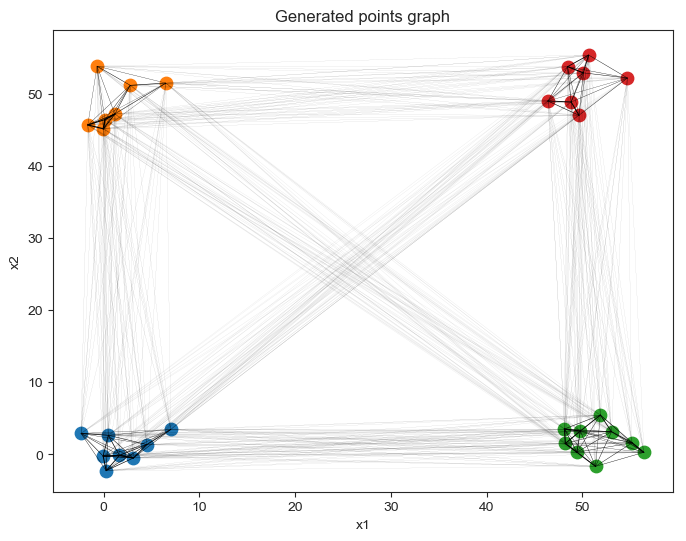
\includegraphics[width=0.8\textwidth]{immagini/clus_fcg.png}%
	}\par\medskip
	\subcaptionbox{\textit{Molten} graph\label{fig:clus:_mg}}{%
		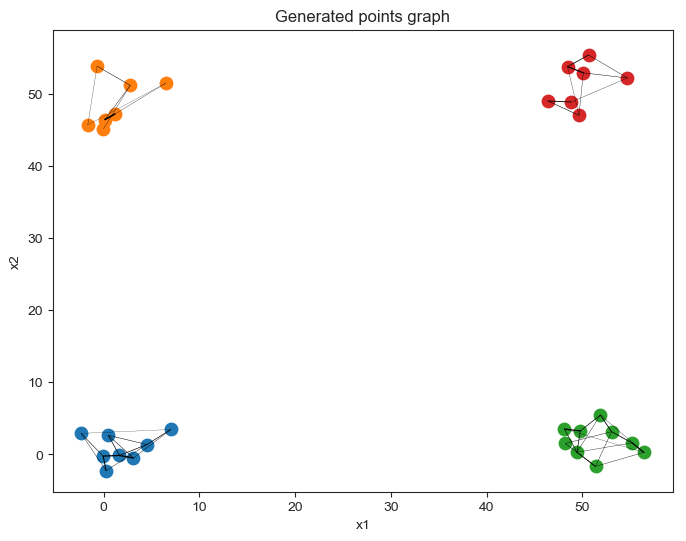
\includegraphics[width=0.8\textwidth]{immagini/clus_mg.png}%
	}
	\caption{Two subsequent stages of the clusters data set generation}
	\label{fig:clus_plots}
\end{figure}

\subsubsection{Single pattern generation}

Once the independent clusters come to form, it is in order to assign each of the nodes a \textbf{topological ordering} in such a way to perform the \textbf{ancestral sampling} (Chapter 16 of Goodfellow, \textit{et al.}, 2016). Since the graphs are directed, in the edges data structure created each edge is in the form of a couple $(i,j)$, i.e. edge from node $i$ to node $j$. Then if one node appears only on the left slot of such representation, it has topological order 1, in that no edge ends up at that node. Conversely, each node appearing on the right has almost one ancestor. For each edge then, each right node is saved to a proper data structure, and it is kept track of the ancestors of each node. In this way it is possible to assign both the topological order and to keep a list of all the ancestors. It will be useful in the stage of sampling to dispose of such list. 

As a zero model however it is done as follows: A data item is initially initialized with all the features values of $-1$. Since each vertex in the graph encodes a feature, and the belongingness of each vertex to a group is an information known from the points generation stage, an integer ranging from 1 to the number of classes $N_c = 4$ is sampled uniformly. The nodes corresponding to this label number are assigned different values, according to their topological order. This is trivial to do since for each vertex belonging to the selected group one simply puts in the corresponding slots in the data vector the topological order of such vertices. 

A further improvement could be rather this approach: once a label is sampled, one could sample from the distribution $p(x_i)$, for the vertices with topological order 1 in that cluster. The values associated with nodes having topological order 2 is still sampled from that distribution, but must be conditioned to the values sampled for their ancestors (nodes of order 1), i.e. $p(x_i \, | \, \text{Ancestors}(x_i))$. This is explained by recalling the very purpose of graphical models: to show (even graphically) the \textit{causality} of the random variables involved. As distribution it could be chosen a Gaussian with mean zero and variance proportional to the degree of that node. Gaussian is believed to fit since nearby features are expected to have similar values (Kemp, 2008, but differently from this work, here one does not generate the features vector, hence sampling from the multivariate Gaussian having zero mean and variance dependent on the inverse of the Laplacian matrix of the graph. Here it suffices to sample a value for a single node, and hence the degree of a node could be a good compromise, being such quantity one of the ingredients of the Laplacian).

The following nomenclatural convention is adopted: vectors are \textbf{\textit{bold-italic}} typefaced, such as one single data item. Since all the entries are random variables, in this case one refers to a single entry of the data item vector as $x_i$, even if it is widespread to typeface random variables with roman capitalisation. So in the following $p(x_i)$ refers to the probability associated with the outcome $x_i$ of the random variable that is encoded by the $i$-th entry of the data item.

To sample from the conditional $p(x_i\, | \, \text{Ancestors}(x_i))$ the following rationale may be implemented: The distribution is referred to all the nodes up to $i$, then could be viewed as a multivariate distribution. Then a value is sampled from that multivariate distribution, but keeping constants the values of the random variables sampled yet. As an example: Assume that node 3 of cluster 1 is to be assigned the value $x_3$ and that $\text{Ancestors}(x_3) = [1,2]$. Then the pdf to sample from is 

\begin{equation}
	\displaystyle p(x_3 \, | \, x_1, x_2) \sim \exp \left( - \frac{1}{2} (x_1, x_2, x_3)^T \, \bm{\Sigma}^{-1} \, (x_1, x_2, x_3) \right)
\end{equation}

with $\bm{\Sigma} = \text{diag}(k_i)$, $i = 1, \dots, \ 3$, being $k_i$ the degree of node $i$. The above formula may be broken in products, owing to the fact that the variance matrix is diagonal, that is 

\begin{equation}
	\begin{array}{r c l}
		\displaystyle p(x_3 \, | \, x_1, x_2) &\sim& \exp \left(-\dfrac{1}{2} \dfrac{x_1^2}{k_1^2}\right) \, \exp \left(-\dfrac{1}{2} \dfrac{x_2^2}{k_2^2}\right) \, X_3 \\[3mm] %\exp \left(\frac{1}{2} \frac{x_3^2}{k_3^2}\right) \\[1mm]
		X_3 &\sim& \mathcal{N}\left( 0, k_3^{-2} \right)
	\end{array}
\end{equation}

the first two factors being \textbf{the values} that the Gaussian probability density function attains at the values sampled for the ancestors $x_1$ and $x_2$ and the third factor is the value sampled from the Gaussian having zero mean and variance $k_3^2$.

\subsubsection{Complete data set}

This procedure is repeated many times as specified by the user. Here a good number is, as in the case of binary tree, $M = 2000$ items. In the complete data set hence one has features in which the only values not being $-1$ lay in correspondence of the indexes of the data array that match with the nodes of the graph that belongs to the category given by the label of that feature. Labels are again \textit{one-hot} vectors. For example, assume that the first cluster is selected. If this first cluster comprises the vertices ranging from 1 to 5, where node 1 has order 1, 2 and 3 have order 2, 4 has order 3 and five has order 4, then that data item has values $[1, 2, 2, 3, 4, -1, \dots, \ -1]$ and the corresponding label is $[1, 0, \dots\ , 0]$.


\begin{algorithm}
	\begin{algorithmic}[1]
		\caption{Independent clusters. Simulated melting to \textit{partition the graph}}
		
		\State Choose the number of classes $N_C$
		\State Set $\bm{\mu}^{(k)} \in \mathbb{R}^2$, $\bm{\Sigma}^{(k)} \in \mathbb{R}^{2\times2}$, $k = 1, \dots, N_C$
		\State Generate $\bm{X}$ s.t. $\bm{x}_i \sim \mathcal{N}(\bm{\mu}^{(k)}, \bm{\Sigma}^{(k)})$, $i = 1, \dots, M$
		\State Include the indexes of the points generate in a list, which is the set of the vertices $\mathcal{V}$ of the graph $\mathcal{G}$
		\State Fully connect the vertices to form a fully connected graph and group the vertices and the set of the edges $\mathcal{E}$ in the graph data structure, $\mathcal{G} = \{\mathcal{V}, \mathcal{E}\}$. \textbf{Note} that since 2-dimensional coordinates will be useful, $\mathcal{V}$ is a dictionary of keys (nodes indexes $i = 1, \dots, M$) and values (list with the point coordinates, $(x_i^{(1)}, x_i^{(2)})$).
		
		\For {$T$ increasing}
		
		\For {All the edges $e = 1,\dots, |\mathcal{E}|$}
		
		\If {Length of edge $e > \frac{1}{T}$ (for example) }
		
		\State Remove edge $e$
		\EndIf
		\EndFor
		\EndFor
		
		\State Plot the remaining edges and check if only independent fully connected components have survived.
		\label{alg:simulatedmelting}
	\end{algorithmic}
\end{algorithm}


\begin{algorithm}
	\begin{algorithmic}[1]
		\caption{Independent clusters. Single pattern generation}
		\State Here $i$ indexes a single random variable. This kernel is used as many times as the number of samples the user wants to generate. $\bm{x}$ is the whole data item, initialised with each slot set to $-1$.
		\State Set $\bm{x}$ = $\{-1\}^N$
		\State Sample $L \sim \mathcal{U}(\{ 1, \dots, N_c\})$
		\For {all the vertices $i = 1,\dots, n_k$ in cluster $L$}
			\If {Topological Order of $i$ is 1}
				\State $x_i \sim p(x_i) \sim \mathcal{N}(0, k_i^{-2})$
			\Else
				\State $x_i \sim p(x_i) \, \prod_{j \in \text{Ancestors}(x_i)} (4\pi \, k_j^2)^{-1/2}\, \exp \left(-\dfrac{1}{2} \dfrac{x_j^2}{k_j^2} \right)$ 
			\EndIf
		\EndFor
		\State $\bm{y}_i = \text{one-hot}(L)$
		
		\label{alg:clus_spg}
	\end{algorithmic}
\end{algorithm}

\begin{figure}[t!]
	\begin{subfigure}{0.5\textwidth}
		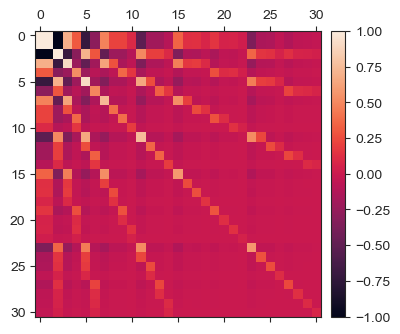
\includegraphics[scale=0.8]{immagini/tree_cov.png}
		\caption{Binary tree data set}
		\label{fig:tree_cov}
	\end{subfigure}
	\hspace{2mm}
	\begin{subfigure}{0.5\textwidth}
		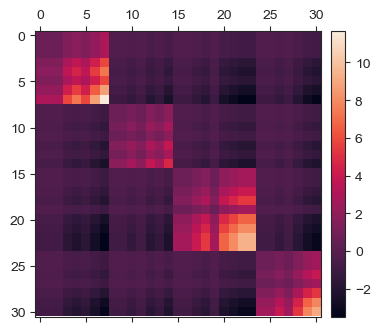
\includegraphics[scale=0.8]{immagini/clus_cov.png}
		\caption{Clusters data set}
		\label{fig:clus_cov}
	\end{subfigure}
	\caption{Covariances matrices visualisation of the two different data sets.}
	\label{fig:covs}
\end{figure}




\section{Neural network model}
\label{secc:system}

The two data sets are hand-crafted to have the same number of features and overall classes. This choice could be flexible however. The program that implements the simulation is capable to self-adjust the number of neurons according to the input size and the categories number. First table below gives an overview of the network architecture. The second table reports the setting of the optimization algorithm used.

\begin{table}[h!]
	\begin{center}
		\begin{tabular}{r l l}
			Architecture  & & \\
			Layer         & Units    & Activation \\
			\hline
			1 (input)     & $N = 31$ & -          \\
			2 (hidden)    & 20       & ReLU       \\
			3 (hidden)    & 10       & ReLU       \\
			4* (output)    & 4        & Softmax    \\
		\end{tabular}
	\end{center}
\end{table}


\begin{table}[h!]
	\begin{center}
		\begin{tabular}{r l}
			NASGD        & \\
			\hline
			Learing rate & 0.01 \\
			Decay        & $10^{-6}$ \\
			Momentum     & 0.6
		\end{tabular}
	\end{center}
\end{table}

\section{Results}

It is not striking that the model learns in just few iterations to classify correctly the samples. Data sets are easily tractable, in particular the clusters data sets. Here the systems sees non-$-1$ values in correspondence of a class, then it is straight forward to learn what is the underlying pattern, regardless the fact that the non-$-1$ values are real numbers, if one implements an ancestral sampling using normal distributions, or as in the present case, where features are simply the topological order of the vertices.

\begin{figure}[t!]
	\centering
	\subcaptionbox{Binary tree data set\label{fig:tree_performance}}{%
		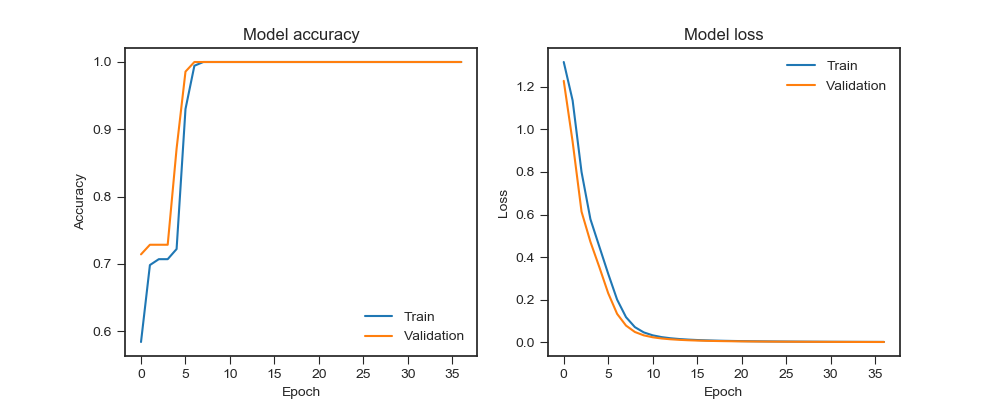
\includegraphics[width=1\textwidth]{immagini/tree_performance.png}%
	}\par\medskip
	\subcaptionbox{Independent clusters data set\label{fig:clus_performance}}{%
		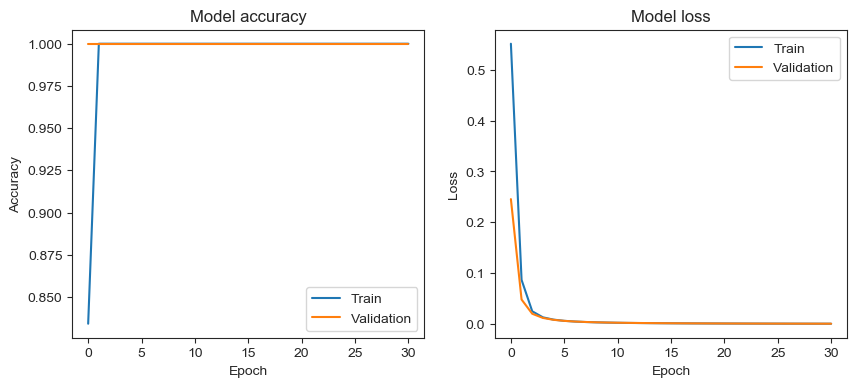
\includegraphics[width=1\textwidth]{immagini/clus_performance.png}%
	}
	\caption{Performance of the system on different data sets.}
	\label{fig:nn_perf}
\end{figure}


\subsection{Binary tree data set}

The simple neural network illustrated is trained with the data set. A 0.7 fraction is used for training, a 0.1 of which is used as validation set, and the 0.3 kept apart before is used as test set. Being the data set linearly separable, in few epochs the accuracy metric attains the top value of 1.0.

\begin{table}[h!]
	\begin{center}
		\begin{tabular}{r l}
			Test set accuracy     & 1.0 \\
			Test set loss         & 0.0017
		\end{tabular}
	\end{center}
\end{table}

As final result, weights and biases distributions are also reported for the trained network, alongside with the connections strengths visualisation, Figure \ref{fig:tree_net_trained}.

%\newpage

%\newpage

\subsection{Independent clusters data set}

Since here the map to be learned from the \textit{states space} (i.e. the domain of the data) to the \textit{target space} is straightforward (it does not take a neural network to understand the game), learning takes two epochs to be over, with a smaller value of the test loss.

\begin{table}[h!]
	\begin{center}
		\begin{tabular}{r l}
			Test set accuracy     & 1.0 \\
			Test set loss         & 0.00080
		\end{tabular}
	\end{center}
\end{table}


\subsection{Modularly varying goals}

It is interesting also to inspect the response of the system once exposed to two different data sets formerly discussed. What is immediately clear is that more motifs are observed, likely due to the fact that the neural network undergoes a longer training stage and then the weights are updated forward the optimum for a prolonged period. The fact that the cost is monotonically decreasing for both the two data sets suggest that even an optimal configuration is found, the cost function hyper-surface resembles a mild hill slope, where the parameters configuration point keeps descending. 


\subsection{Motifs detection}

The \texttt{mfinder1.2} executable program (\href{http://www.weizmann.ac.il/mcb/UriAlon/download/network-motif-software}{documentation here}) is exploited in the next stage, that is inspecting the system in search of significant patterns.

As an introductory note: the weights of the neural network as obtained by the \textsf{Keras} build-in function, are real-valued of course. The cited program only can deal with $+1$ valued edges strengths. Then, as an exploratory experiment, the weights exceeding (both in positive and negative value), a given cutoff threshold, are set to $+1$ and to $0$ otherwise. By thus doing the resulting graph item can be fed to the \texttt{mfinder1.2} program. 

Since the cut-off threshold is arbitrary, it is in order to perform different analyses for different values of such a value. For example, the difference in the results using $C = 0.25$ and $C = 0.35$ is sharp: The former yields the detection off all among the possible motifs, given the architectural constraints, while the latter yields way less motifs. Some sensitivity tests were performed. It turned out that the value of $C = 0.32$ is the \textit{critical point}, which allows for the detection of three motifs, but above such value, say for example 0.35, only one motif can be found. However, the profile of the motifs significance does not vary. If one sets a low threshold, the $Z$-score profiles are similar each other. $Z$-score is defined as 

\begin{equation}
	Z = \dfrac{N_{\text{real}} - <N_{\text{rand}}>}{\sigma_{rand}}
\end{equation}

being $N_{\text{real}}$ the number of counts of a given motifs in the real network, $N_{\text{rand}}$ is the average of such count in an ensemble of randomized networks and $\sigma_{rand}$ its standard deviation. The random networks generation is performed in consistency with the original network features: same nodes, same connectivity and same degree sequence. 

This $Z$-score profile then is not prone to variation, it only exhibits fluctuations in its value for a given motif, but the most recurring subgraphs are always the same. \textbf{Important}: also in the initial weights configuration the profile is the same, with lower values of $Z$-score for each motif. But this could not raise concerns since the initial configuration is generate randomly. For the neural networks learning dynamics itself, for a given initial configuration the weights which are initially greater in magnitude tend to increase and the same applies for the negative valued ones. One of the drawbacks of deep learning models is indeed the fact that a good choice of the initial condition is crucial. The cost function features a plethora of local minima, hence a poor choice of the initial condition may resolve in the system to get stuck in a local minima which nevertheless does not match an optimum. 

In this particular case, data sets are fairly easy to be assimilated by the system, then there is no peril the parameters configuration to wander around this much during the training stage. Then once chosen an initial configuration, the dynamics of learning evolves this latter towards the closest minimum. That is why slightly greater edge weights increase, and the same goes for both positive and negative values. If one takes a look to Figures \ref{fig:tree_net_trained}, \ref{fig:clus_net_trained}, it is clear that the (weighted) topology of the evolved system indeed resembles the initial one. Figure \ref{fig:mvg_net_trained}, as pointed out above, exemplifies the fact that learning \textit{consolidates} the final configurations of both the sub-tasks. In Figures \ref{fig:zsc_0d25}, \ref{fig:zsc_0d32} and \ref{fig:zsc_0d35} $Z$-score profiles for the MVG case resemble the ones of the tree data set cases. It should not be surprising inasmuch MVG is a tree and clusters learning reiterated. But clusters-consequent motifs are a subset of the tree case, so learning the two different tasks in a periodic fashion does not cause the system to change significantly its internal structure in terms of parameters.

\begin{table}[h!]
	\begin{center}
		\begin{tabular}{||p{1cm} | p{1cm} | p{1cm} | p{2.5cm} | p{1.5cm} | p{1.5cm} | p{1cm} | p{1.5cm}||}			
			\hline
			Nodes & Motif ID & $N_{\text{real}}$ & $N_{\text{rand}}$ stats & $N_{\text{real}}$ $Z$-score &  $N_{\text{real}}$ P-val & Unique Val & C real \\
			\hline \hline
			\multicolumn{8}{c}{\textbf{Initial} weights configuration} \\
			\hline
			4 & 14 & 206 & $ 141.6\pm9.2$ & 7.03 & 0.000 &  8  & 26.73   \\
			4 & 28   &   378   & $   271.6\pm18.7   $ &   5.69    &  0.000   &   5    &  49.04     \\ 
			4 & 74   &   915   & $   782.2\pm31.3   $ &   4.25    &  0.000   &   8    &  118.71    \\
			4 & 76   &   2235  & $    1917.9\pm53.5 $ &     5.92  &    0.000 &     12 &     289.96 \\
			4 & 204  &    106  & $    42.5\pm6.1    $ &  10.46    &  0.000   &   9    &  13.75     \\
			4 & 280  &    1019 & $     771.0\pm32.2 $ &     7.70  &    0.000 &     10 &     132.20 \\
			4 & 904  &    159  & $    25.8\pm5.9    $ &  22.54    &  0.000   &   8    &  20.63     \\
			4 & 2184 &     668 & $     547.6\pm17.1 $ &     7.04  &    0.000 &     13 &     86.66  \\
			\hline \hline
			\multicolumn{8}{c}{\textbf{Tree data set}-fed systems weights} \\
			\hline
			4 & 14    &  404    & $ 240.0\pm17.9    $ &     9.19   &   0.000    &  8    &  27.75    \\
			4 & 28    &  757    & $ 479.8\pm32.9    $ &     8.43   &   0.000    &  5    &  52.00    \\
			4 & 74    &  1458   & $  1301.4\pm53.2  $ &    2.95    &  0.010     & 9     & 100.14    \\
			4 & 76    &  3855   & $  3238.1\pm100.0 $ &     6.17   &   0.000    &  12   &   264.78  \\
			4 & 204   &   261   & $  91.7\pm10.1    $ &     16.69  &    0.000   &   11  &    17.93  \\
			4 & 280   &   2046  & $   1408.8\pm62.3 $ &     10.23  &    0.000   &   10  &    140.53 \\ 
			4 & 904   &   432   & $  60.8\pm9.8     $ &      38.06 &     0.000  &    9  &    29.67  \\
			4 & 2184  &    1356 & $    1038.2\pm33.7$ &      9.42  &    0.000   &   14  &    93.14  \\
			\hline \hline
			\multicolumn{8}{c}{\textbf{Clusters data set}-fed systems weights} \\
			\hline
			4 & 14    &  289   &  $ 186.2\pm13.7    $ &  7.51    &  0.000    &  8     & 26.36       \\
			4 & 28    &  585   &  $ 395.3\pm24.0    $ &  7.92    &  0.000    &  5     & 53.36       \\
			4 & 74    &  1232  &  $  1074.7\pm39.4  $ &    3.99  &    0.000  &    8   &   112.38    \\
			4 & 76    &  2913  &  $  2563.9\pm72.9  $ &    4.79  &    0.000  &    12  &    265.71   \\
			4 & 204   &   178  &  $  61.6\pm7.4     $ &   15.78  &    0.000  &    11  &    16.24    \\
			4 & 280   &   1511 &  $   1099.9\pm48.9 $ &     8.42 &     0.000 &     10 &     137.83  \\
			4 & 904   &   281  &  $  42.1\pm7.5     $ &   31.74  &    0.000  &    8   &   25.63     \\
			4 & 2184  &    965 &  $   765.7\pm26.7  $ &    7.45  &    0.000  &    15  &    88.02    \\
			\hline \hline
			\multicolumn{8}{c}{\textbf{MVG-undergone} systems weights} \\
			\hline
			4 & 14   &   629    & $  345.6\pm25.1     $ & 11.31     & 0.000     & 8     & 30.68      \\
			4 & 28   &   1109   & $   651.6\pm43.4    $ &  10.54    &  0.000    &  5    &  54.09     \\
			4 & 74   &   2001   & $   1739.2\pm68.3   $ &   3.84    &  0.000    &  9    &  97.60     \\ 
			4 & 76   &   5365   & $   4508.7\pm118.0  $ &    7.26   &   0.000   &   12  &    261.69  \\ 
			4 & 204  &    505   & $   159.2\pm16.6    $ &  20.79    &  0.000    &  11   &   24.63    \\ 
			4 & 280  &    2943  & $    1890.6\pm86.7  $ &    12.14  &    0.000  &    10 &     143.55 \\ 
			4 & 328  &    1499  & $    1339.0\pm79.9  $ &    2.00   &   0.050   &   4   &   73.12    \\ 
			4 & 904  &    691   & $   93.4\pm13.9     $ & 43.07     & 0.000     & 8     & 33.71      \\ 
			4 & 2184 &     2049 & $     1504.9\pm49.8 $ &     10.92 &     0.000 &     14&      99.95 \\ 
			\hline
		\end{tabular}
	\end{center}
	\caption{Results of the \texttt{mfinder1.2} program for the $C = 0.25$ cut-off threshold.}
\end{table}


\begin{table}[h!]
	\begin{center}
		\begin{tabular}{||p{1cm} | p{1cm} | p{1cm} | p{2.5cm} | p{1.5cm} | p{1.5cm} | p{1cm} | p{1.5cm}||}			
			\hline
			Nodes & Motif ID & $N_{\text{real}}$ & $N_{\text{rand}}$ stats & $N_{\text{real}}$ $Z$-score &  $N_{\text{real}}$ P-val & Unique Val & C real \\
			\hline \hline
			\multicolumn{8}{c}{\textbf{Initial} weights configuration} \\
			\hline
			4 &28   & 73   & $ 61.3\pm5.3     $ & 2.19 & 0.000 & 4  & 70.06   \\
			4 &280  &  137 & $   120.7\pm6.9  $ & 2.35 & 0.000 & 10 &  131.48 \\
			4 &392  &  350 & $   266.1\pm17.6 $ & 4.75 & 0.000 & 8  & 335.89  \\
			\hline \hline
			\multicolumn{8}{c}{\textbf{Tree data set}-fed systems weights} \\
			\hline
			4 & 14   & 45    & $ 29.4\pm4.1      $ & 3.81  & 0.000  & 6   & 11.91   \\
			4 & 28   & 264   & $  193.3\pm16.0   $ & 4.41  & 0.000  & 5   & 69.86   \\
			4 & 76   & 723   & $  613.4\pm34.7   $ & 3.16  & 0.000  & 9   & 191.32  \\
			4 & 204  &  30   & $  8.3\pm2.7      $ & 7.90  & 0.000  & 7   & 7.94    \\
			4 & 280  &  534  & $   425.6\pm24.7  $ & 4.38  & 0.000  & 10  &  141.31 \\
			4 & 392  &  1129 & $    832.6\pm43.4 $ & 6.83  & 0.000  & 9   & 298.76  \\
			4 & 904  &  92   & $  11.6\pm3.8     $ & 21.43 &  0.000 &  6  &  24.35  \\
			4 & 2184 &   318 & $    267.4\pm12.6 $ & 4.00  & 0.000  & 12  &  84.15  \\
			\hline \hline
			\multicolumn{8}{c}{\textbf{Clusters data set}-fed systems weights} \\
			\hline
			4 & 14   & 23    & $ 16.9\pm2.9     $ & 2.13  & 0.010  & 6   &11.05    \\
			4 & 28   & 138   & $  109.7\pm9.2   $ & 3.07  & 0.000  & 5   &66.28    \\
			4 & 204  &  14   & $  3.3\pm1.7     $ & 6.14 &  0.000 &  4  & 6.72    \\
			4 & 280  &  285  & $   241.5\pm14.0 $ & 3.10 &  0.000 &  10 &  136.89 \\
			4 & 392  &  632  & $   499.6\pm29.6 $ & 4.48 &  0.000 &  8  & 303.55  \\
			4 & 904  &  40   & $  5.3\pm2.3     $ & 14.78 &  0.000 &  6  & 19.21   \\
			4 & 2184 &   151 & $    132.7\pm7.1 $ & 2.58 &  0.000 &  13 &  72.53  \\
			\hline \hline
			\multicolumn{8}{c}{\textbf{MVG-undergone} systems weights} \\
			\hline
			4 & 14   & 68    & $ 43.6\pm6.1       $ & 3.97  & 0.000 & 5  & 14.41   \\
			4 & 28   & 316   & $  224.1\pm19.5    $ & 4.71  & 0.000 & 5  & 66.95   \\
			4 & 76   & 961   & $  822.1\pm49.4    $ & 2.81  & 0.000 & 10 &  203.60 \\
			4 & 204  &  42   & $  13.3\pm3.6      $ & 7.89  & 0.000 & 7  & 8.90    \\
			4 & 280  &  667  & $   513.2\pm30.0   $ & 5.12  & 0.000 & 10 &  141.31 \\
			4 & 392  &  1331 & $    1002.1\pm56.9 $ & 5.78  & 0.000 & 8  & 281.99  \\
			4 & 904  &  123  & $   14.9\pm4.1     $ & 26.58 & 0.000 & 6  & 26.06   \\
			4 & 2184 &   411 & $    341.4\pm17.2  $ & 4.03  & 0.000 & 12 &  87.08  \\
			\hline
		\end{tabular}
	\end{center}
	\caption{Results of the \texttt{mfinder1.2} program for the $C = 0.32$ cut-off threshold.}
\end{table}


\begin{table}[h!]
	\begin{center}
		\begin{tabular}{||p{1cm} | p{1cm} | p{1cm} | p{2.5cm} | p{1.5cm} | p{1.5cm} | p{1cm} | p{1.5cm}||}			
			\hline
			Nodes & Motif ID & $N_{\text{real}}$ & $N_{\text{rand}}$ stats & $N_{\text{real}}$ $Z$-score &  $N_{\text{real}}$ P-val & Unique Val & C real \\
			\hline \hline
			\multicolumn{8}{c}{\textbf{Initial} weights configuration} \\
			\hline
			4 & 392 & 195 & $ 128.8+-15.1 $ & 4.38  & 0.000 & 8 & 397.96 \\
			\hline \hline
			\multicolumn{8}{c}{\textbf{Tree data set}-fed systems weights} \\
			\hline
			4 & 14    & 23     & $  16.1\pm2.4      $ &  2.84  & 0.000  & 5  &  10.20   \\
			4 & 28    & 152    & $   117.4\pm10.7   $ &  3.23  & 0.000  & 5  &  67.38   \\
			4 & 76    & 419    & $   357.6\pm22.8   $ &  2.69  & 0.010  & 9  &  185.73  \\
			4 & 204   &  11    & $   3.8\pm2.0      $ &  3.60  & 0.010  & 4  &  4.88    \\
			4 & 280   &  313   & $     255.3\pm18.9 $ &  3.05  & 0.000  & 9  &  138.74  \\
			4 & 392   &  710   & $     511.3\pm37.0 $ &  5.37  & 0.000  & 7  &  314.72  \\
			4 & 904   &  57    & $     6.1\pm2.6    $ &  19.35 &  0.000 &  6 &   25.27  \\
			4 & 2184  &   193  & $     167.8\pm9.2  $ &  2.74  & 0.000  & 11 &   85.55  \\
			\hline \hline
			\multicolumn{8}{c}{\textbf{Clusters data set}-fed systems weights} \\
			\hline
			4 & 28   & 71   & $ 58.5\pm6.0     $ & 2.09 & 0.020 & 4  & 59.76  \\
			4 & 280  &  163 & $   142.6\pm10.1 $ & 2.01 & 0.020 & 10 & 137.21 \\
			4 & 392  &  390 & $   293.7\pm28.0 $ & 3.44 & 0.000 & 8  & 328.28 \\
			\hline \hline
			\multicolumn{8}{c}{\textbf{MVG-undergone} systems weights} \\
			\hline
			4 & 14    &   31     & $  20.4\pm3.1      $ &  3.48   &  0.000  &  5   &  11.46  \\
			4 & 28    &   192    & $   141.8\pm12.7   $ & 3.95    & 0.000   & 5    &  70.95  \\
			4 & 76    &   490    & $   426.1\pm25.1   $ & 2.55    & 0.000   & 9    &  181.08 \\
			4 & 204   &    23    & $   5.3\pm2.3      $ &  7.72   &  0.000  &  4   &  8.50   \\
			4 & 280   &    379   & $    303.3\pm17.8  $ &  4.27   &  0.000  &  9   &  140.06 \\
			4 & 392   &    819   & $    590.5\pm38.9  $ &  5.88   &  0.000  &  8   &  302.66 \\
			4 & 904   &    72    & $   7.4\pm2.9      $ &  22.16  &   0.000 &   5  &  26.61  \\
			4 & 2184  &     229  & $     193.9\pm10.1 $ &   3.47  &   0.000 &   10 &  84.63  \\
			\hline
		\end{tabular}
	\end{center}
	\caption{Results of the \texttt{mfinder1.2} program for the $C = 0.35$ cut-off threshold.}
\end{table}


\begin{figure}
	\centering
	\begin{subfigure}[b]{0.475\textwidth}
		\centering
		\includegraphics[width=\textwidth]{immagini/init_zsc_0d25}
		\caption[]%
		{{\small $Z$-scores for the \textbf{untrained system}}}    
		\label{fig:init_zsc_0d25}
	\end{subfigure}
	\hfill
	\begin{subfigure}[b]{0.475\textwidth}  
		\centering 
		\includegraphics[width=\textwidth]{immagini/tree_zsc_0d25}
		\caption[]%
		{{\small $Z$-scores for the \textbf{tree data set}-fed system}}    
		\label{fig:tree_zsc_0d25}
	\end{subfigure}
	\vskip\baselineskip
	\begin{subfigure}[b]{0.475\textwidth}   
		\centering 
		\includegraphics[width=\textwidth]{immagini/clus_zsc_0d25}
		\caption[]%
		{{\small $Z$-scores for the \textbf{clusters data set}-fed system}}    
		\label{fig:clus_zsc_0d25}
	\end{subfigure}
	\quad
	\begin{subfigure}[b]{0.475\textwidth}   
		\centering 
		\includegraphics[width=\textwidth]{immagini/mvg_zsc_0d25}
		\caption[]%
		{{\small $Z$-scores for the \textbf{MVG-undergone} system}}    
		\label{fig:mvg_zsc_0d25}
	\end{subfigure}
	\caption[  ]
	{\small Cut-off threshold $C = 0.25$} 
	\label{fig:zsc_0d25}
\end{figure}

\begin{figure}
	\centering
	\begin{subfigure}[b]{0.475\textwidth}
		\centering
		\includegraphics[width=\textwidth]{immagini/init_zsc_0d32}
		\caption[]%
		{{\small $Z$-scores for the \textbf{untrained system}}}    
		\label{fig:init_zsc_0d32}
	\end{subfigure}
	\hfill
	\begin{subfigure}[b]{0.475\textwidth}  
		\centering 
		\includegraphics[width=\textwidth]{immagini/tree_zsc_0d32}
		\caption[]%
		{{\small $Z$-scores for the \textbf{tree data set}-fed system}}    
		\label{fig:tree_zsc_0d32}
	\end{subfigure}
	\vskip\baselineskip
	\begin{subfigure}[b]{0.475\textwidth}   
		\centering 
		\includegraphics[width=\textwidth]{immagini/clus_zsc_0d32}
		\caption[]%
		{{\small $Z$-scores for the \textbf{clusters data set}-fed system}}    
		\label{fig:clus_zsc_0d32}
	\end{subfigure}
	\quad
	\begin{subfigure}[b]{0.475\textwidth}   
		\centering 
		\includegraphics[width=\textwidth]{immagini/mvg_zsc_0d32}
		\caption[]%
		{{\small $Z$-scores for the \textbf{MVG-undergone} system}}    
		\label{fig:mvg_zsc_0d32}
	\end{subfigure}
	\caption[  ]
	{\small Cut-off threshold $C = 0.32$} 
	\label{fig:zsc_0d32}
\end{figure}

\begin{figure}
	\centering
	\begin{subfigure}[b]{0.475\textwidth}
		\centering
		\includegraphics[width=\textwidth]{immagini/init_zsc_0d35}
		\caption[]%
		{{\small $Z$-scores for the \textbf{untrained system}}}    
		\label{fig:init_zsc_0d35}
	\end{subfigure}
	\hfill
	\begin{subfigure}[b]{0.475\textwidth}  
		\centering 
		\includegraphics[width=\textwidth]{immagini/tree_zsc_0d35}
		\caption[]%
		{{\small $Z$-scores for the \textbf{tree data set}-fed system}}    
		\label{fig:tree_zsc_0d35}
	\end{subfigure}
	\vskip\baselineskip
	\begin{subfigure}[b]{0.475\textwidth}   
		\centering 
		\includegraphics[width=\textwidth]{immagini/clus_zsc_0d35}
		\caption[]%
		{{\small $Z$-scores for the \textbf{clusters data set}-fed system}}    
		\label{fig:clus_zsc_0d35}
	\end{subfigure}
	\quad
	\begin{subfigure}[b]{0.475\textwidth}   
		\centering 
		\includegraphics[width=\textwidth]{immagini/mvg_zsc_0d35}
		\caption[]%
		{{\small $Z$-scores for the \textbf{MVG-undergone} system}}    
		\label{fig:mvg_zsc_0d35}
	\end{subfigure}
	\caption[  ]
	{\small Cut-off threshold $C = 0.35$} 
	\label{fig:zsc_0d35}
\end{figure}





\section{Conclusions and remarks}
\label{sec:conclusions}

A decision on the cut-off threshold must now be taken. On the basis of the observation of Figures \ref{fig:tree_hist} to \ref{fig:mvg_kde}, one spots that the weights distributions tails arrive at $\sim \pm 0.5$ in the first layer, $\sim \pm 1.0$ in the second layer and $\sim \pm 1.5$ in the last layer. A low cut-off does not affect any of these while a value of $C = 0.35$ yet cuts off many of the connections in the first layer. This latter is thought to be the less representative, in fact its weights distributions are not undergoing a sharp variation. Instead, the weights distribution of the third layer changes way more, rendering longer tails. The trade-off is the following: A value of $C = 0.25$ eliminate all of those edges with small weights, but a consistent majority is spared, in terms of variety of weight values. 

A choice of $C = 0.35$ on the other hand suffices to erase the majority of the edges, and the ones survived are those associated with a greater strength, both in positive and negative sign. This cut-off, moreover, hides almost all the possible motifs detectable in the initial configuration, as in Figure \ref{fig:init_zsc_0d35}, where only one subgraph is appreciated. This scenario would be the most desirable, in that it reflects the absence of motifs in the initial status and the detection of a large spectrum in the final stage of training. \textbf{But this may seem, in a sense, a forced result}. Such a choice is arbitrary. Might one want to keep the $C = 0.25$ case, which is by no means forbid, he/she would not observe great differences between the initial and final configurations. 

Let, however, be admissible the choice of $C = 0.35$. As pointed out in Figure \ref{fig:tree_zsc_0d35}, binary tree data set-fed neural network exhibits a greater number of motifs, both in diversity and in quantity of patterns found. In particular, the \textit{diamond} motif (id204) is the mostly occurring one. 

To sketch an hypothesis, one could start from Figure \ref{fig:covs}, in which sharply different structures of the covariance matrices are appreciable. While \ref{fig:tree_cov} shows a periodic pattern in the covariances between random variables in the tree structure, thus meaning that there are no such variables which do not share anything with some others, Figure \ref{fig:clus_cov} clearly shows that there are some blocks within which correlation may be found while all of the variables inter-blocks are not correlated. Recall that neural network owe their power and seemingly almightiness to their capacity to extract the statistical features of the data set. In turn, it seems to fit neatly that a less \textit{trivial} statistical signature translates in a more entangled topology in the evolved system. In the binary tree, being this structure hierarchical \textit{per se}, all of the nodes are dependent by the outcome of the root node, thus correlation embraces almost all of the random variables. On the other hand, the independent clusters data set show a simple statistical morphology, a \textbf{sparser}, glassier covariance matrix, and then it comes with no surprise that the motifs detected are less, and less statistically significant. In this sense, less abstraction is required for the model to understand the underlying nature of the data set.

It is also worth a glance to the MVG-undergone system in Figure \ref{fig:mvg_zsc_0d35}. In this case, a new motif showed up (id28) and again the diamond and the \textit{bifan} (id 904 and 204 respectively) are the motifs that are more frequently observed. Referring to Figure \ref{fig:mvg_kde_L3}, it could be spotted a greater \textit{diffusion} of the initial weights distribution, which means that the connection of the last layer experience a greater increase of magnitude. However, the fact that an unseen motifs pop up should not be matter of concern: If one repeats the simulations many times, he/she may appreciate some fluctuations in the results.

\textbf{As a final remark}, in the MVG case, even if it is observed the mentioned weights increase, there are no edges exhibiting much greater values. This may suggest that the different statistical signatures of the chosen data sets are different enough not to enforce certain network motifs, indeed related to one particular statistical structure.


\subsection{Further improvements}

At the present stage the main concern can not be ignored any further: The instrument used to detect network patterns needs to be enhanced in such a way to include the edges strengths information in the motifs inspection stage. The next step in this work then is to create from scratch a procedure to accomplish such a task. Some literature is available for the sake of motif mining in weighted network, see e.g. \href{https://ieeexplore.ieee.org/document/6406443}{Choodbar \textit{et al.}, (2012)} and \href{https://arxiv.org/pdf/cond-mat/0408629.pdf}{Onnela \textit{et al.}, (2004)}.



\begin{figure}[h!]
	\centering
	\subcaptionbox{First layer\label{fig:tree_hist_L1}}{%
		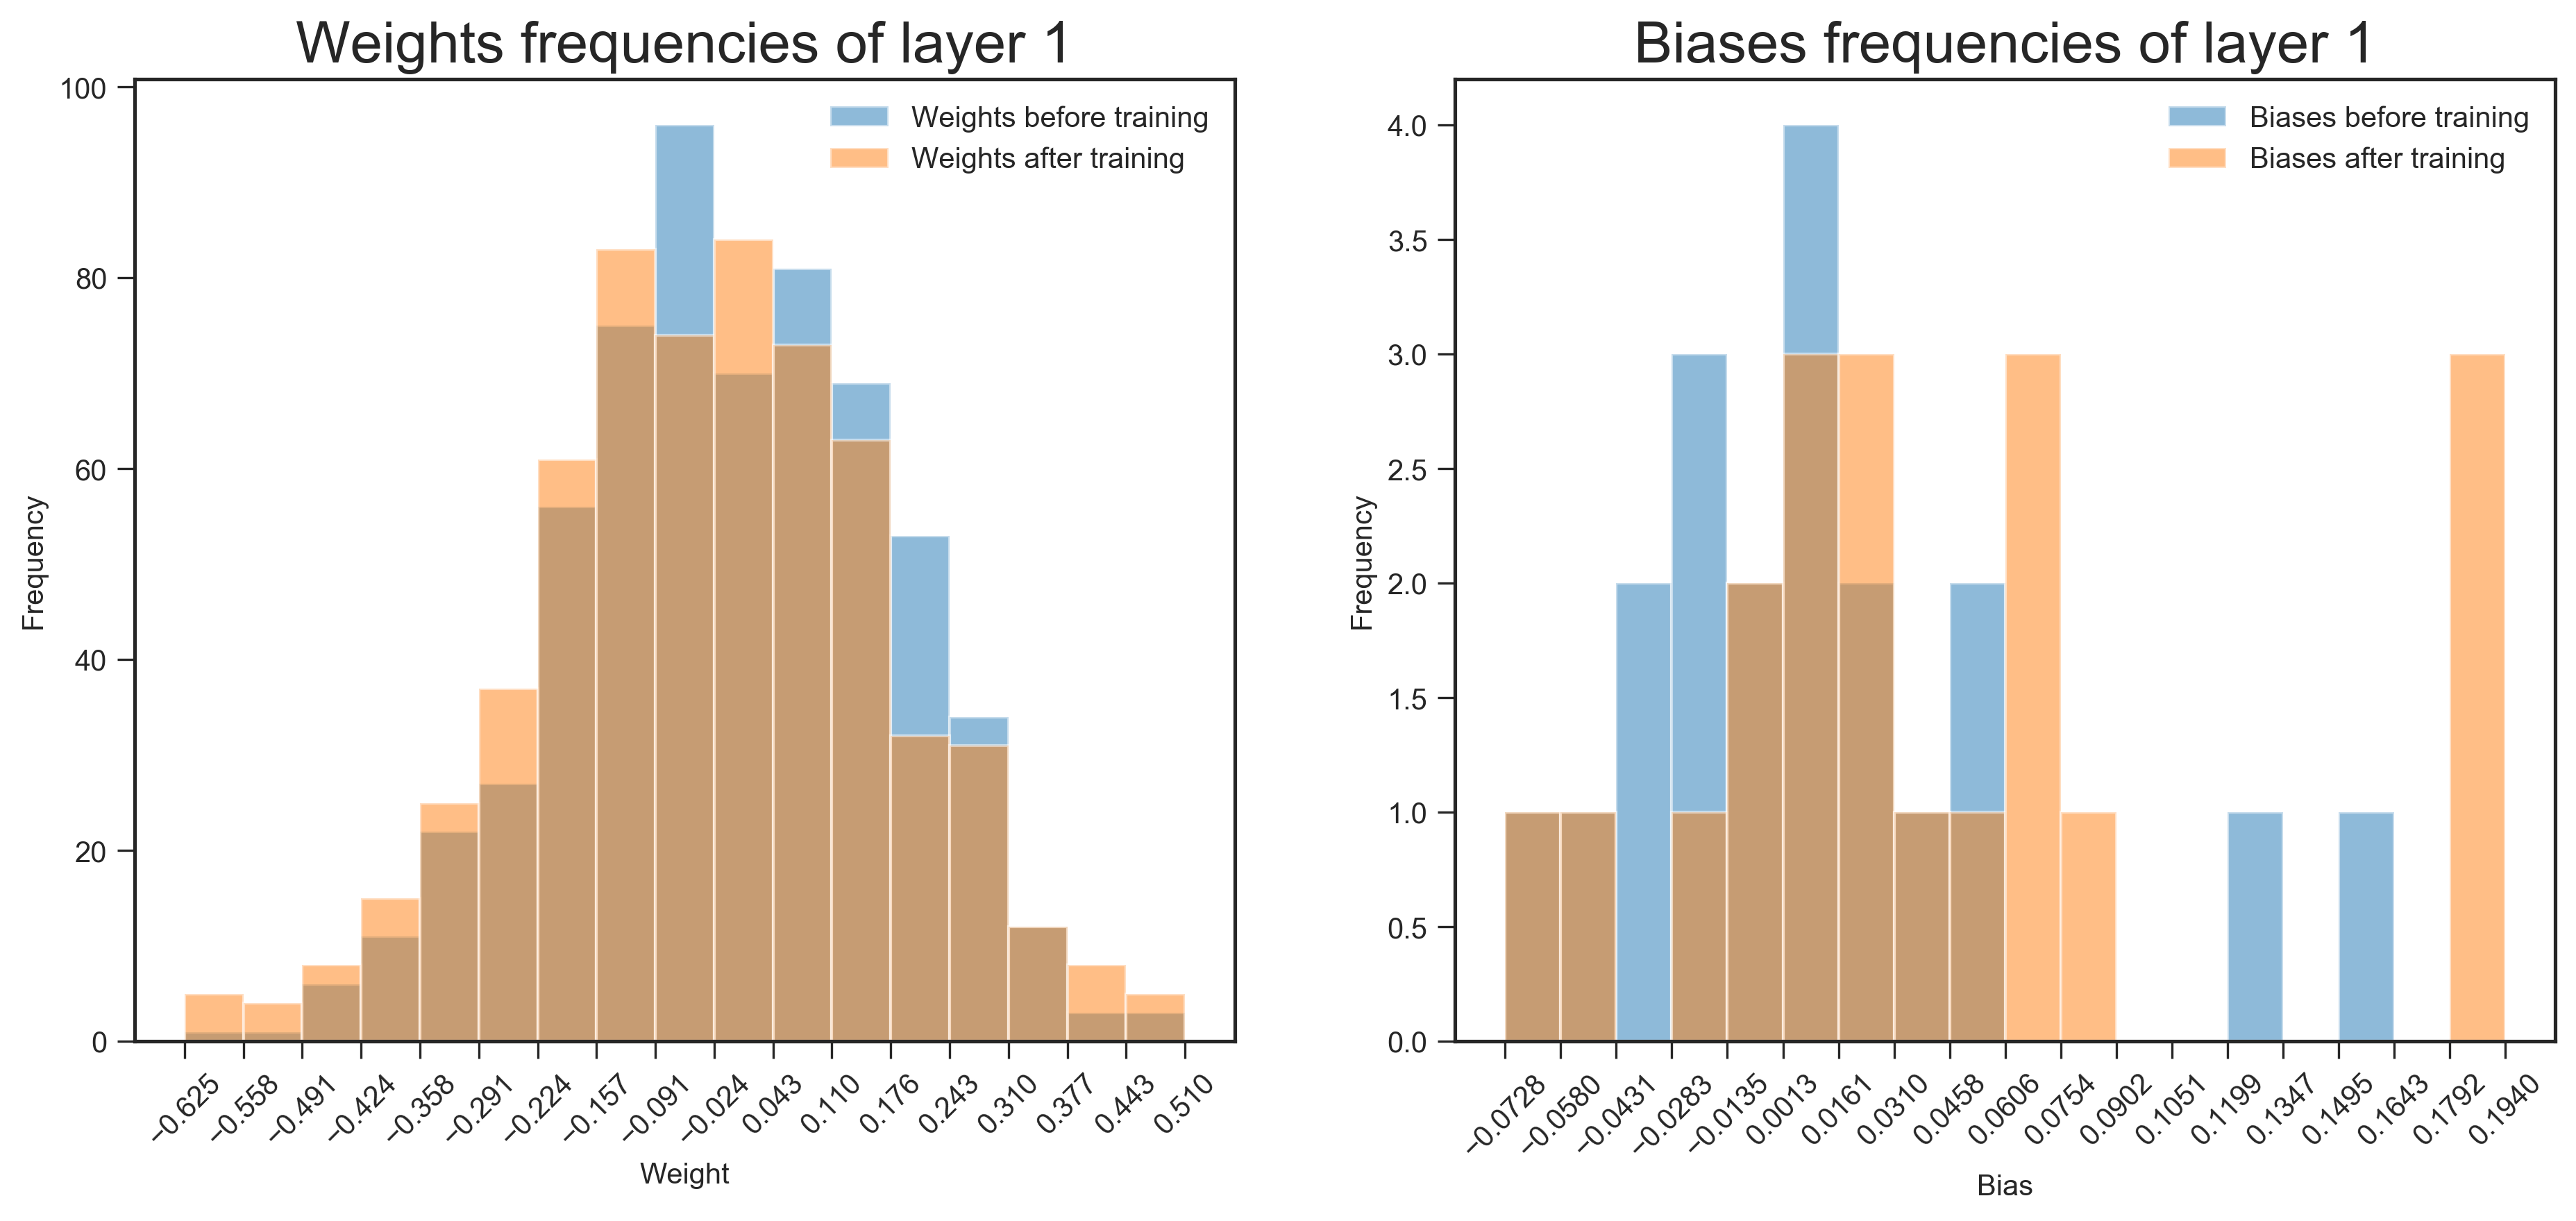
\includegraphics[width=0.9\textwidth]{immagini/tree_hist_L1.png}%
	}\par\medskip
	\subcaptionbox{Second layer\label{fig:tree_hist_L2}}{%
		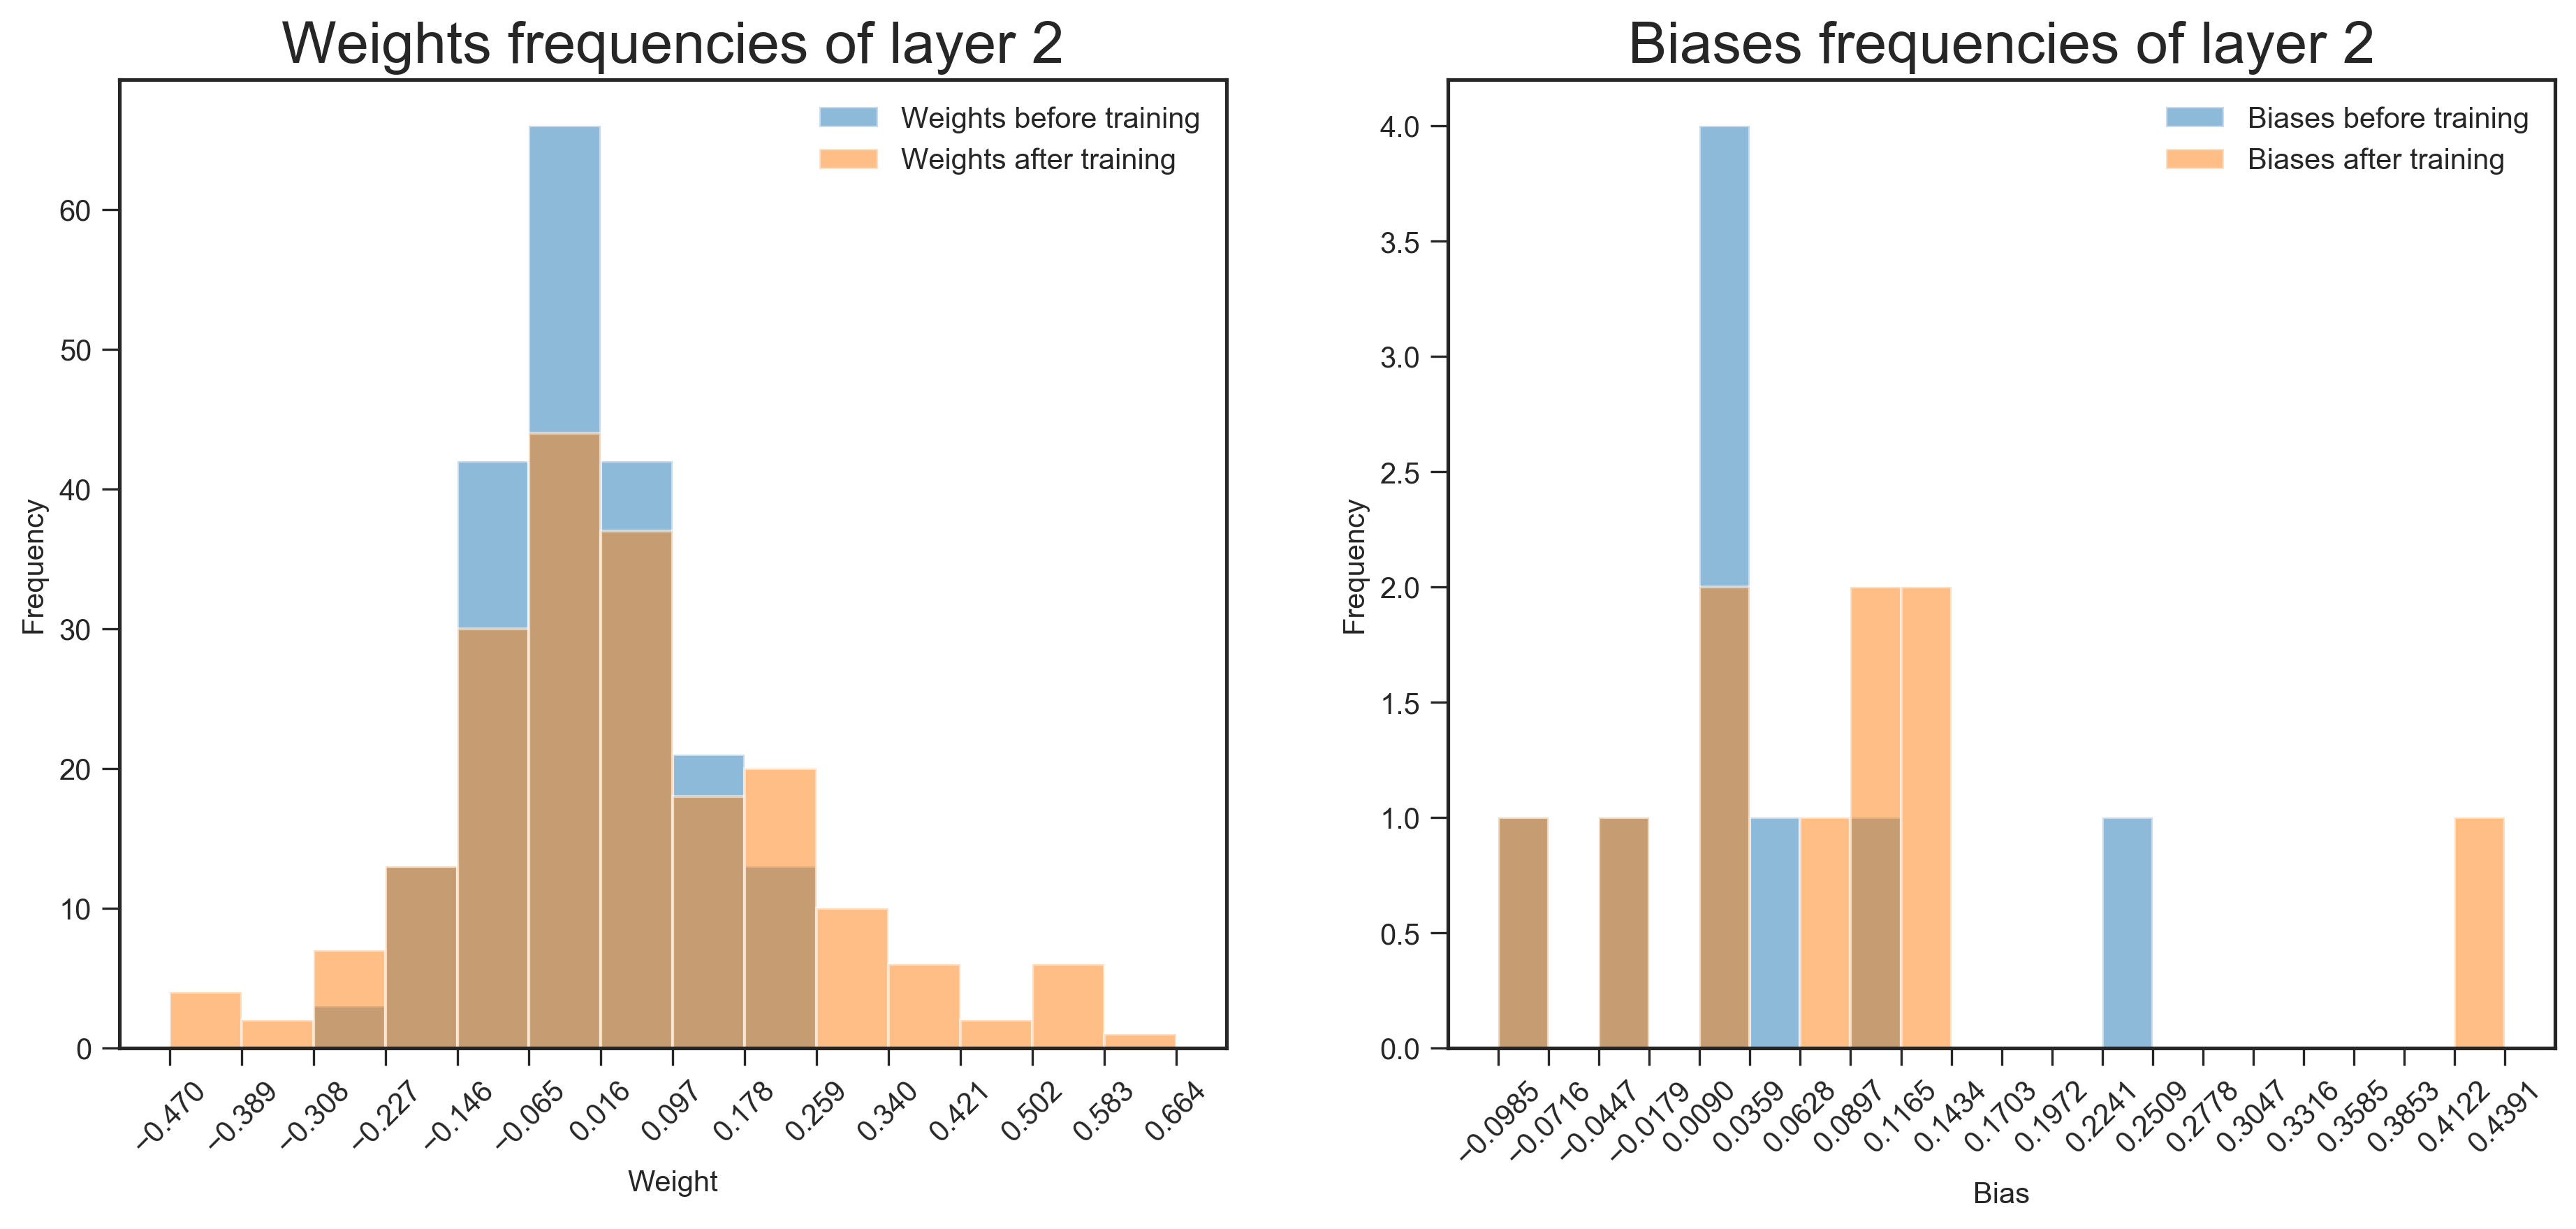
\includegraphics[width=0.9\textwidth]{immagini/tree_hist_L2.png}%
	}\par\medskip        
	\subcaptionbox{Third layer\label{fig:tree_hist_L3}}{%
		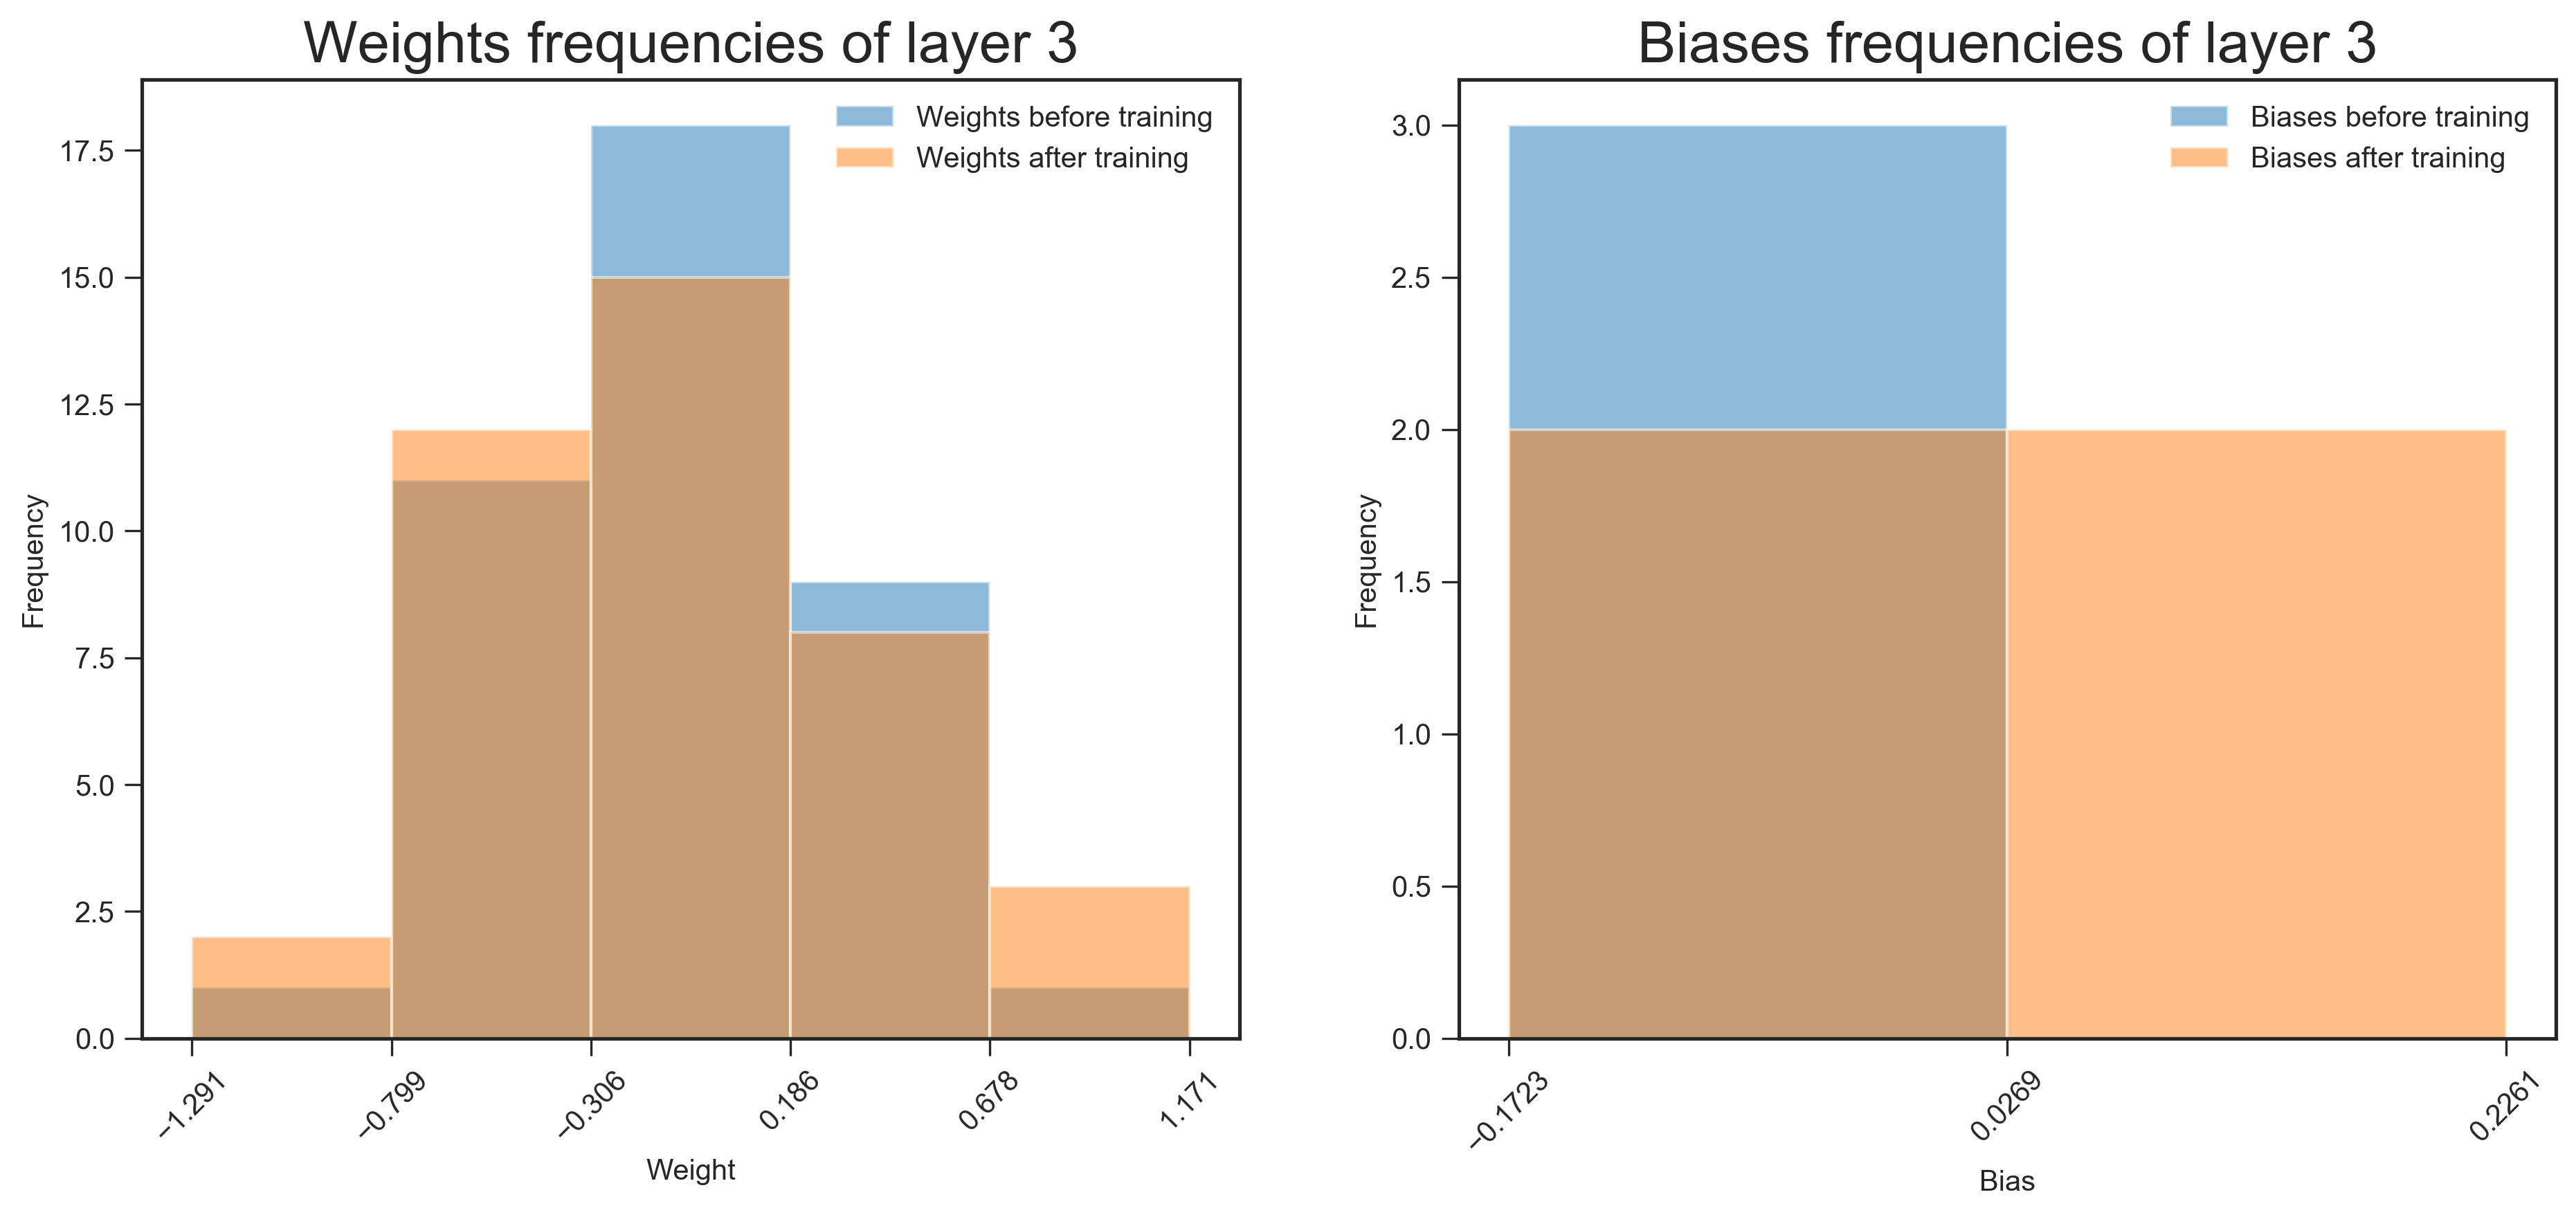
\includegraphics[width=0.9\textwidth]{immagini/tree_hist_L3.png}%
	}
	\caption{Frequency plots of the parameters before and after training. Binary tree data set.}
	\label{fig:tree_hist}
\end{figure}

\begin{figure}[h!]
	\centering
	\subcaptionbox{First layer\label{fig:tree_kde_L1}}{%
		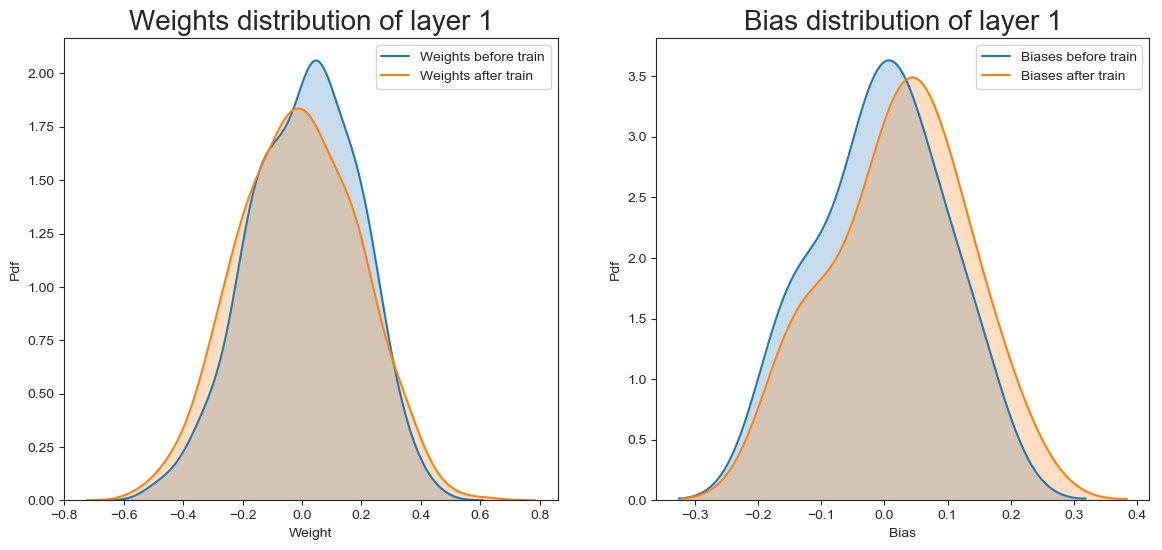
\includegraphics[width=0.9\textwidth]{immagini/tree_kde_L1.png}%
	}\par\medskip
	\subcaptionbox{Second layer\label{fig:tree_kde_L2}}{%
		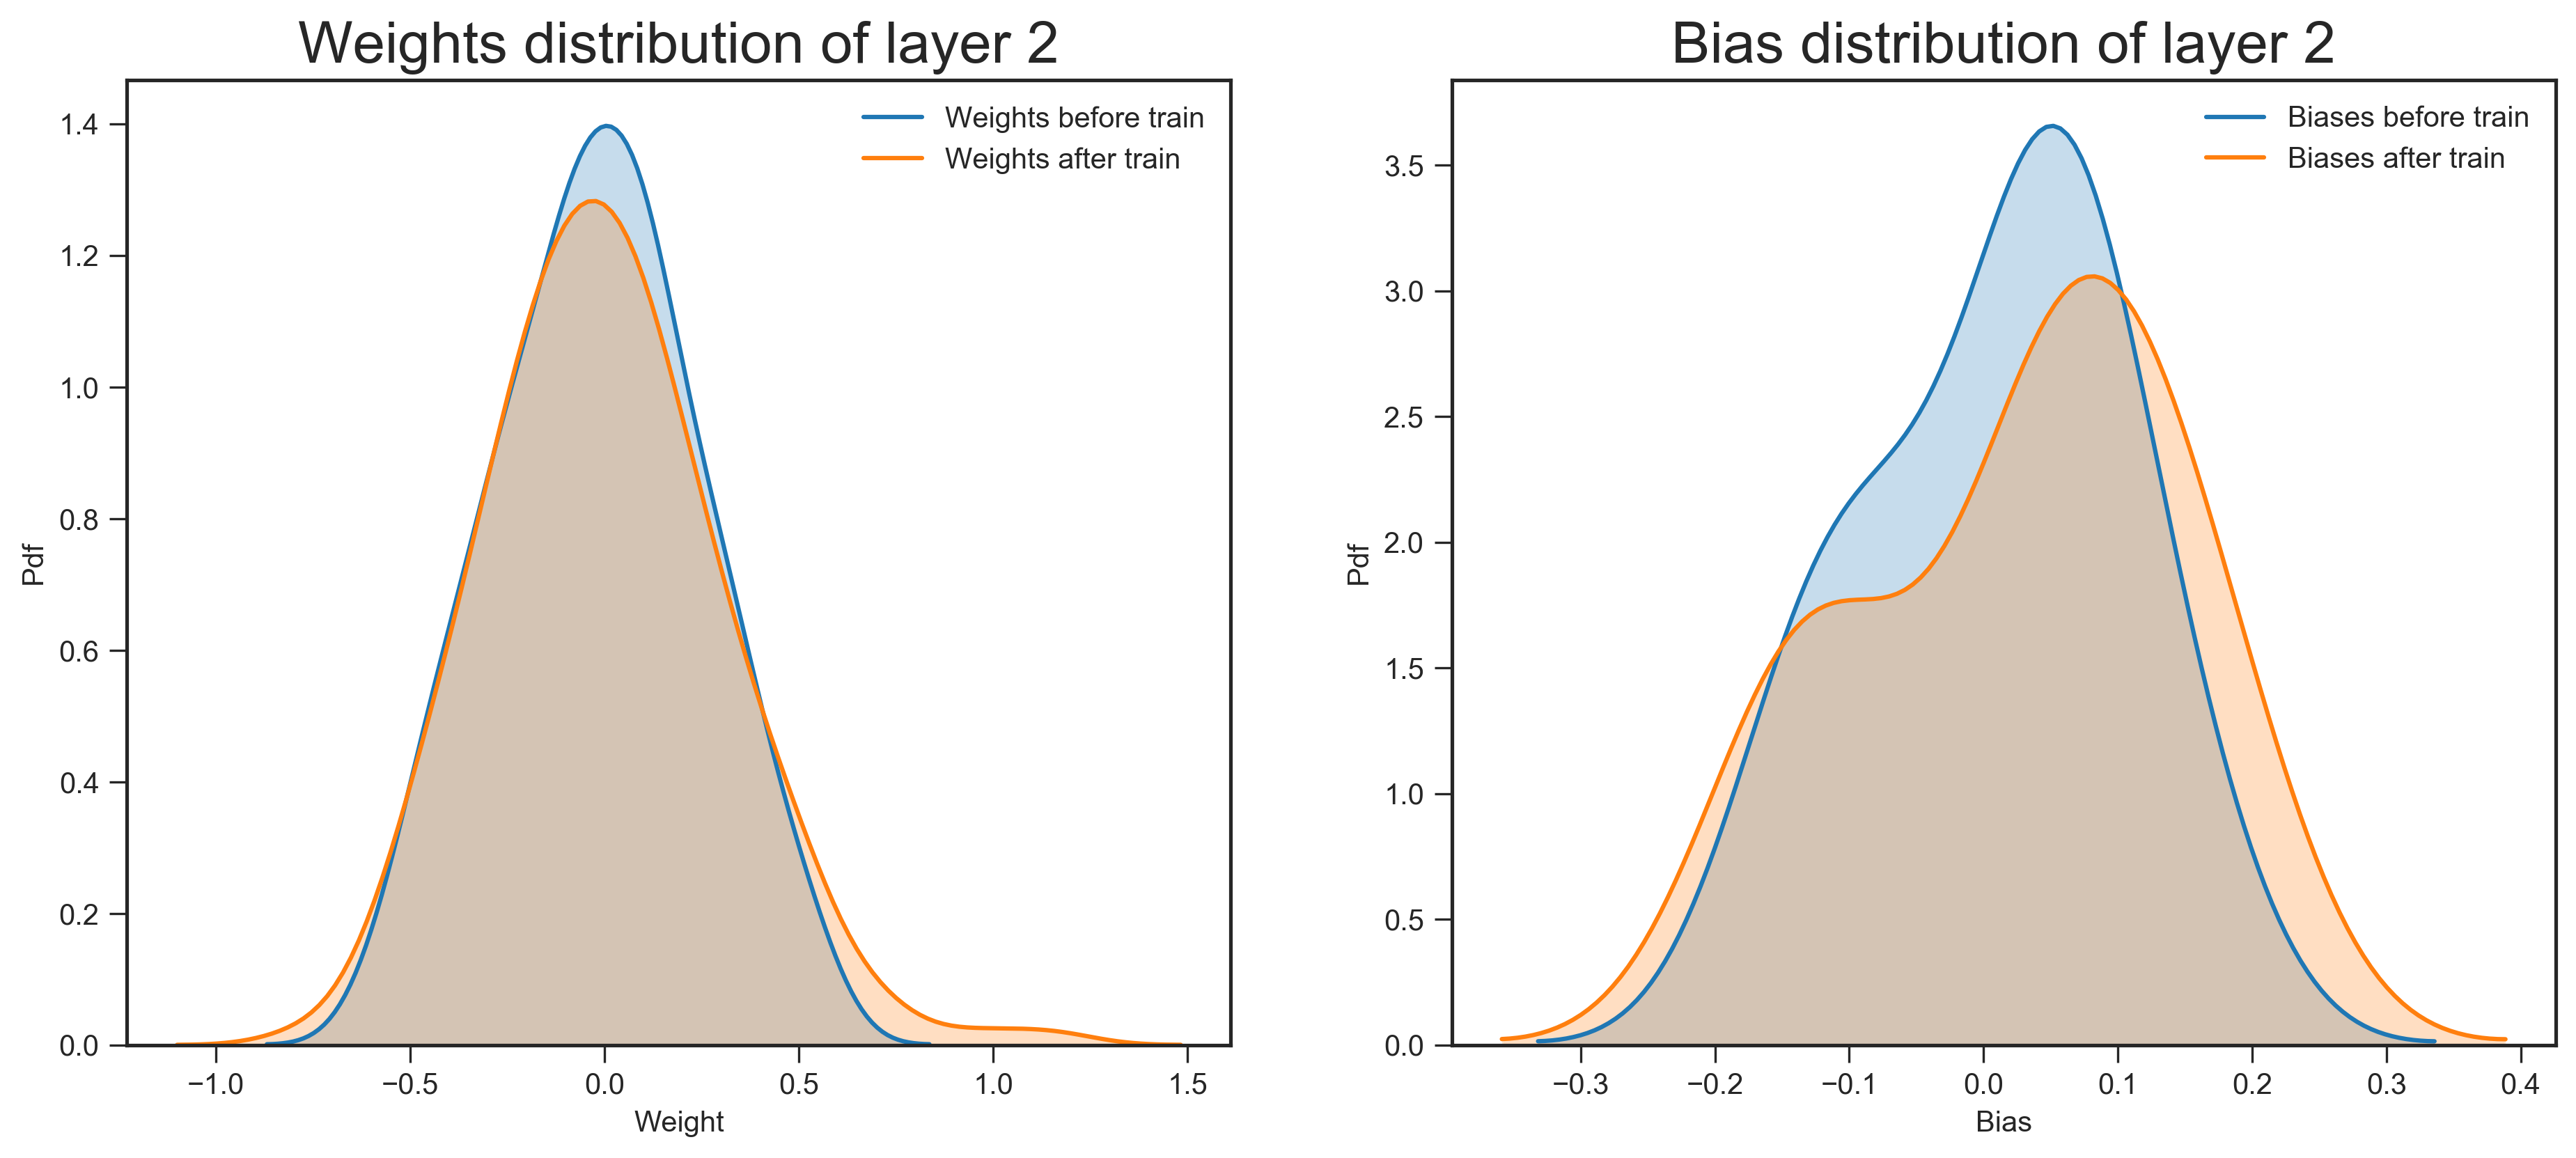
\includegraphics[width=0.9\textwidth]{immagini/tree_kde_L2.png}%
	}\par\medskip        
	\subcaptionbox{Third layer\label{fig:tree_kde_L3}}{%
		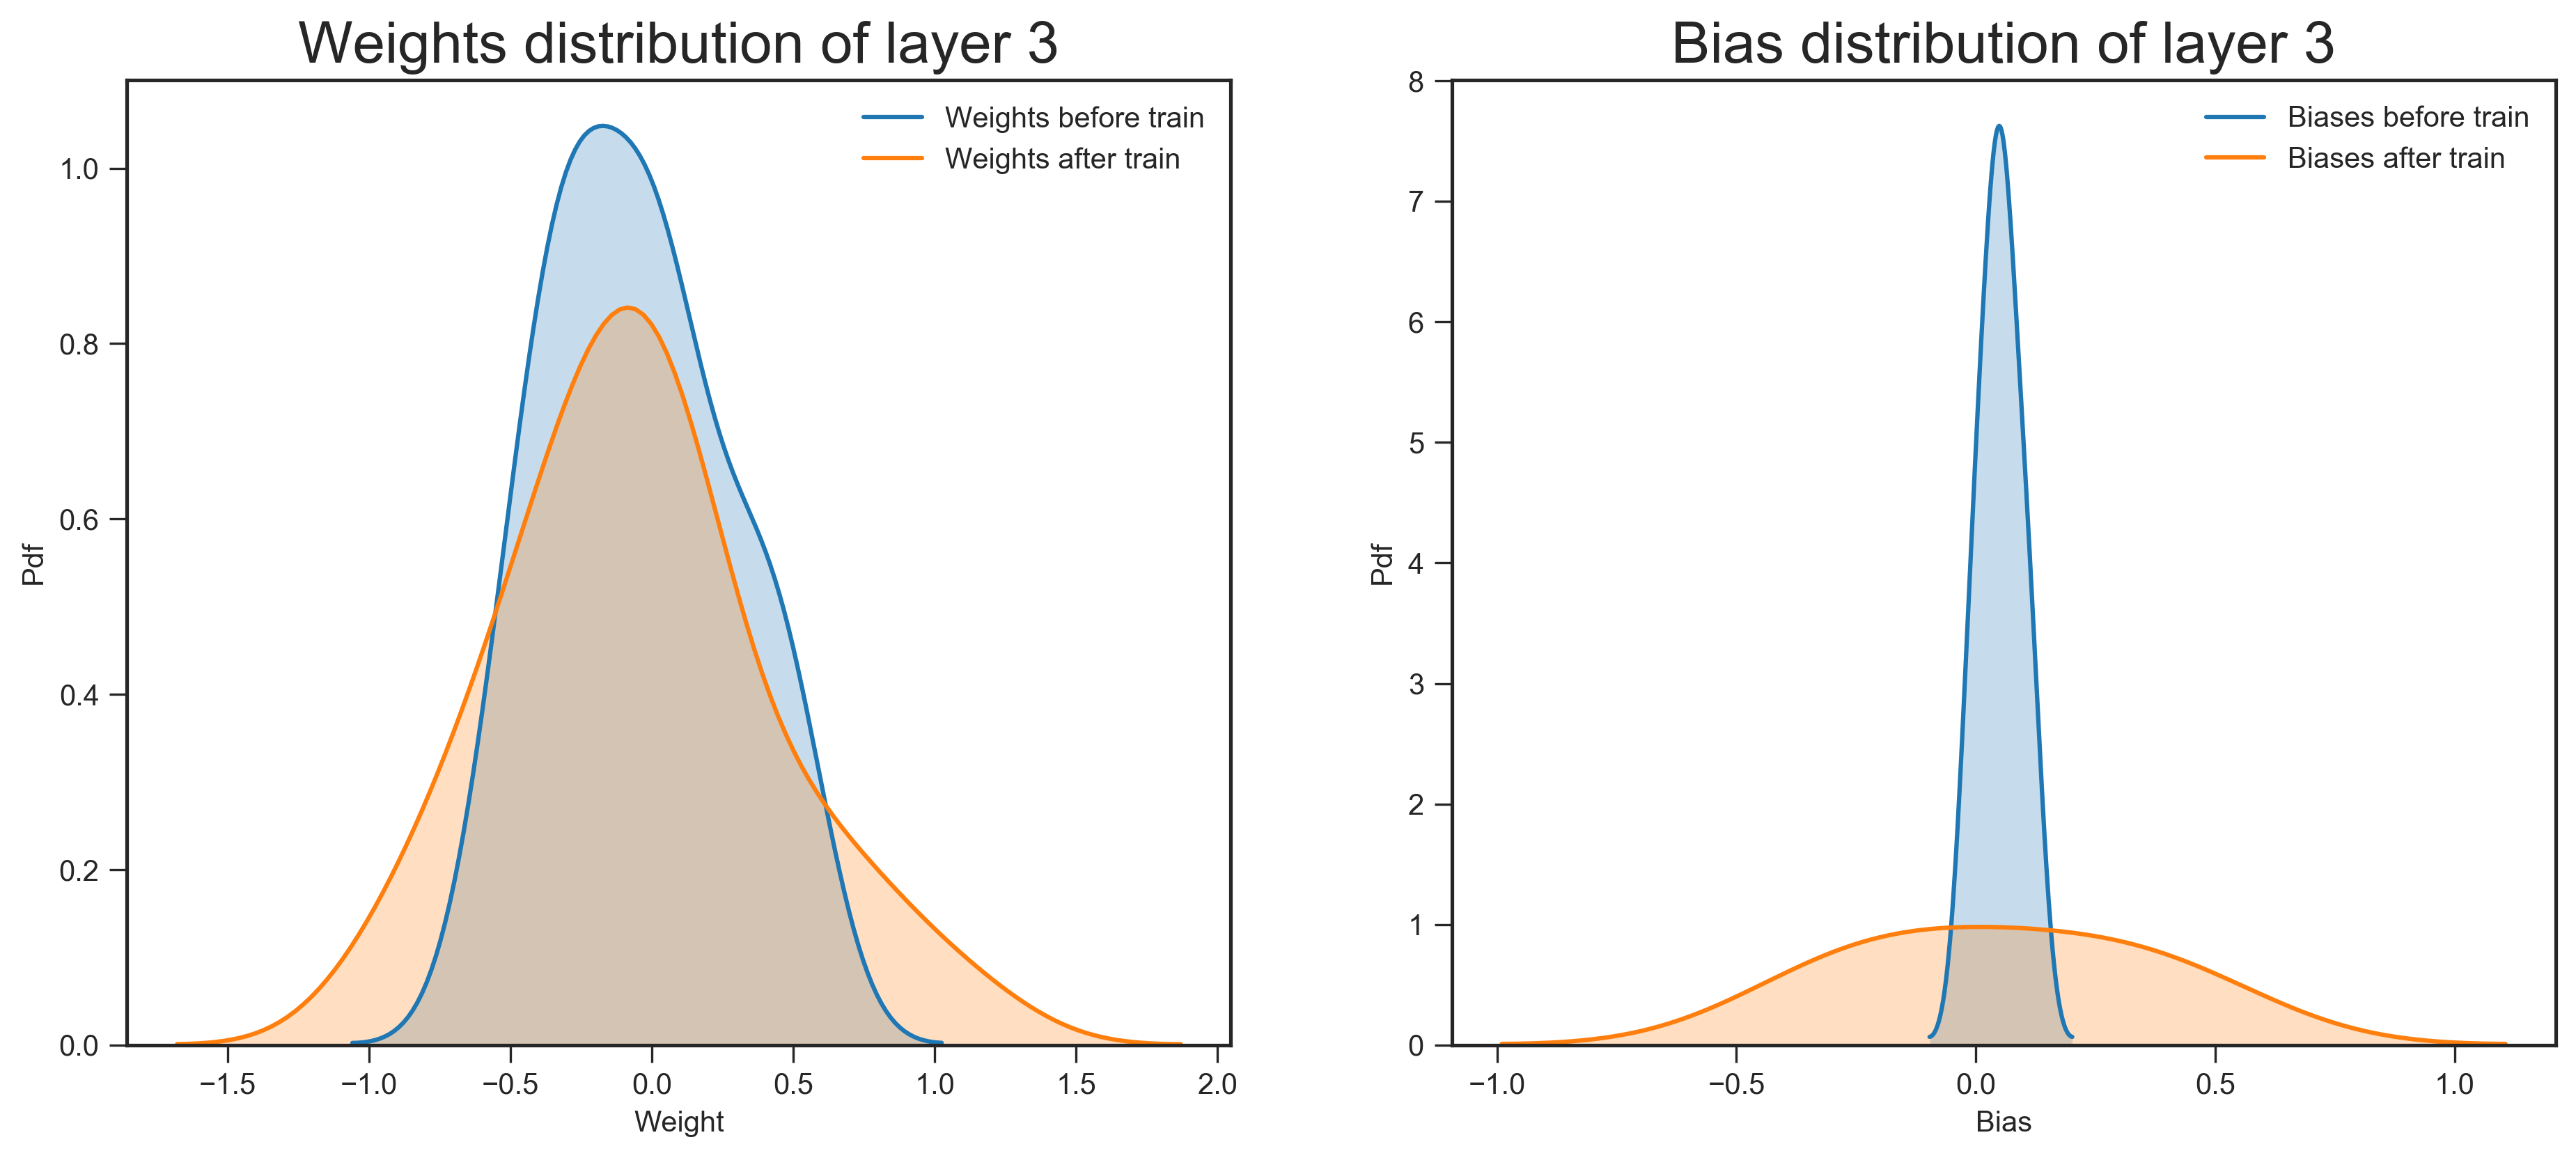
\includegraphics[width=0.9\textwidth]{immagini/tree_kde_L3.png}%
	}
	\caption{KDE plots of the parameters before and after training. Binary tree data set.}
	\label{fig:tree_kde}
\end{figure}

\begin{figure}[h!]
	\centering
	\subcaptionbox{First layer\label{fig:clus_hist_L1}}{%
		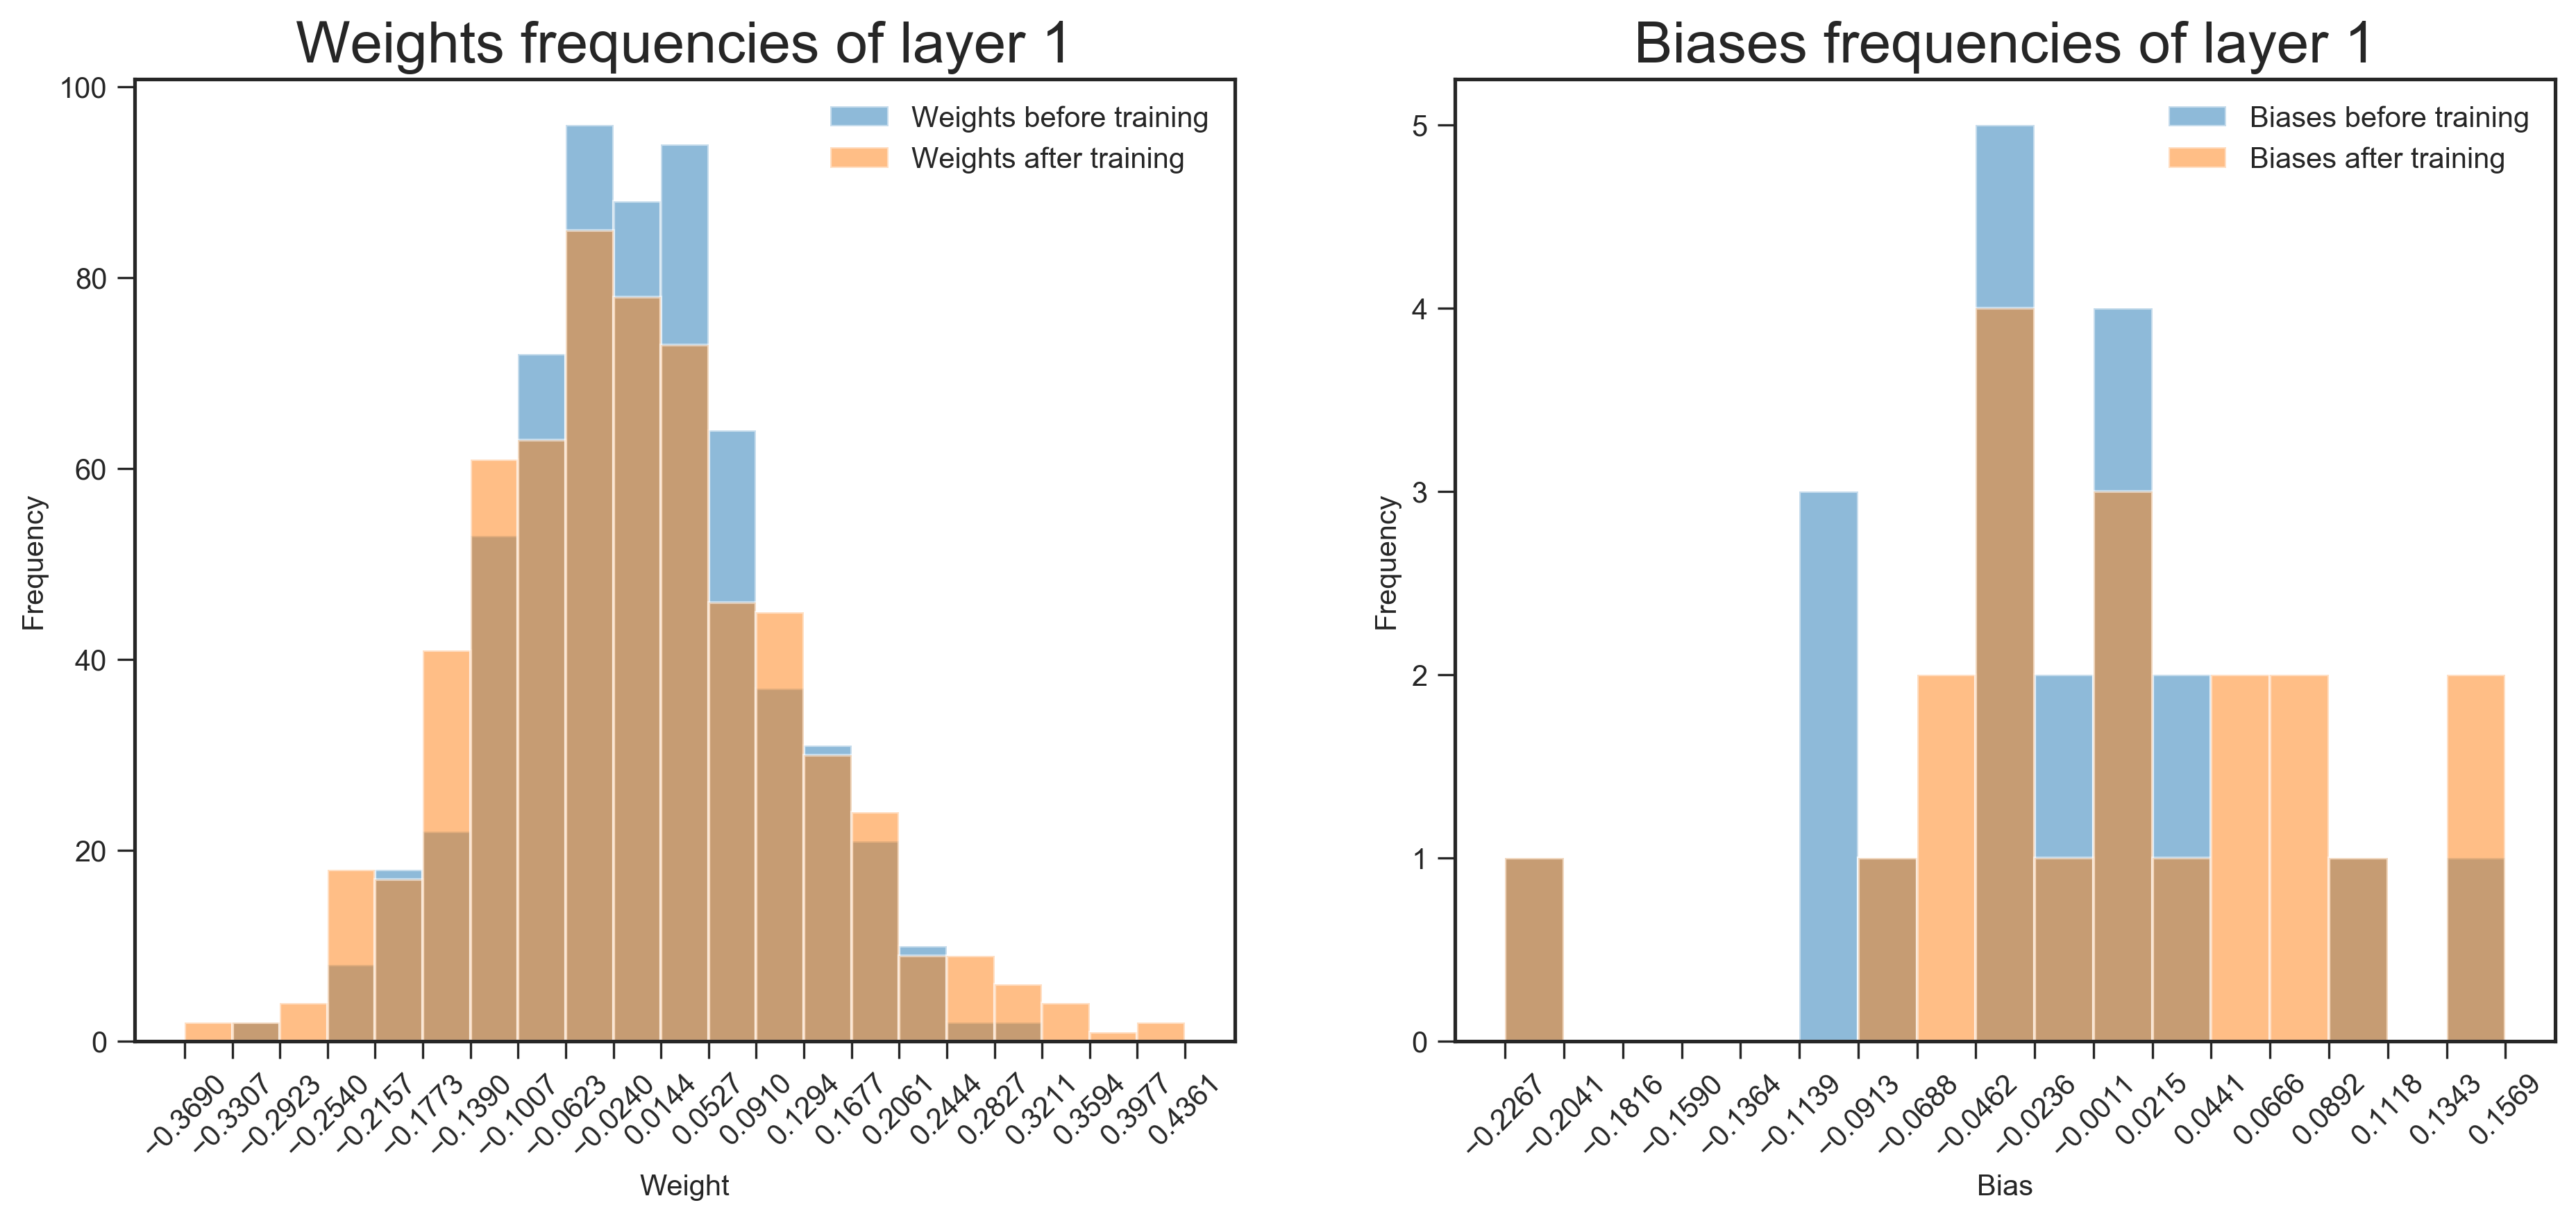
\includegraphics[width=0.9\textwidth]{immagini/clus_hist_L1.png}%
	}\par\medskip
	\subcaptionbox{Second layer\label{fig:clus_hist_L2}}{%
		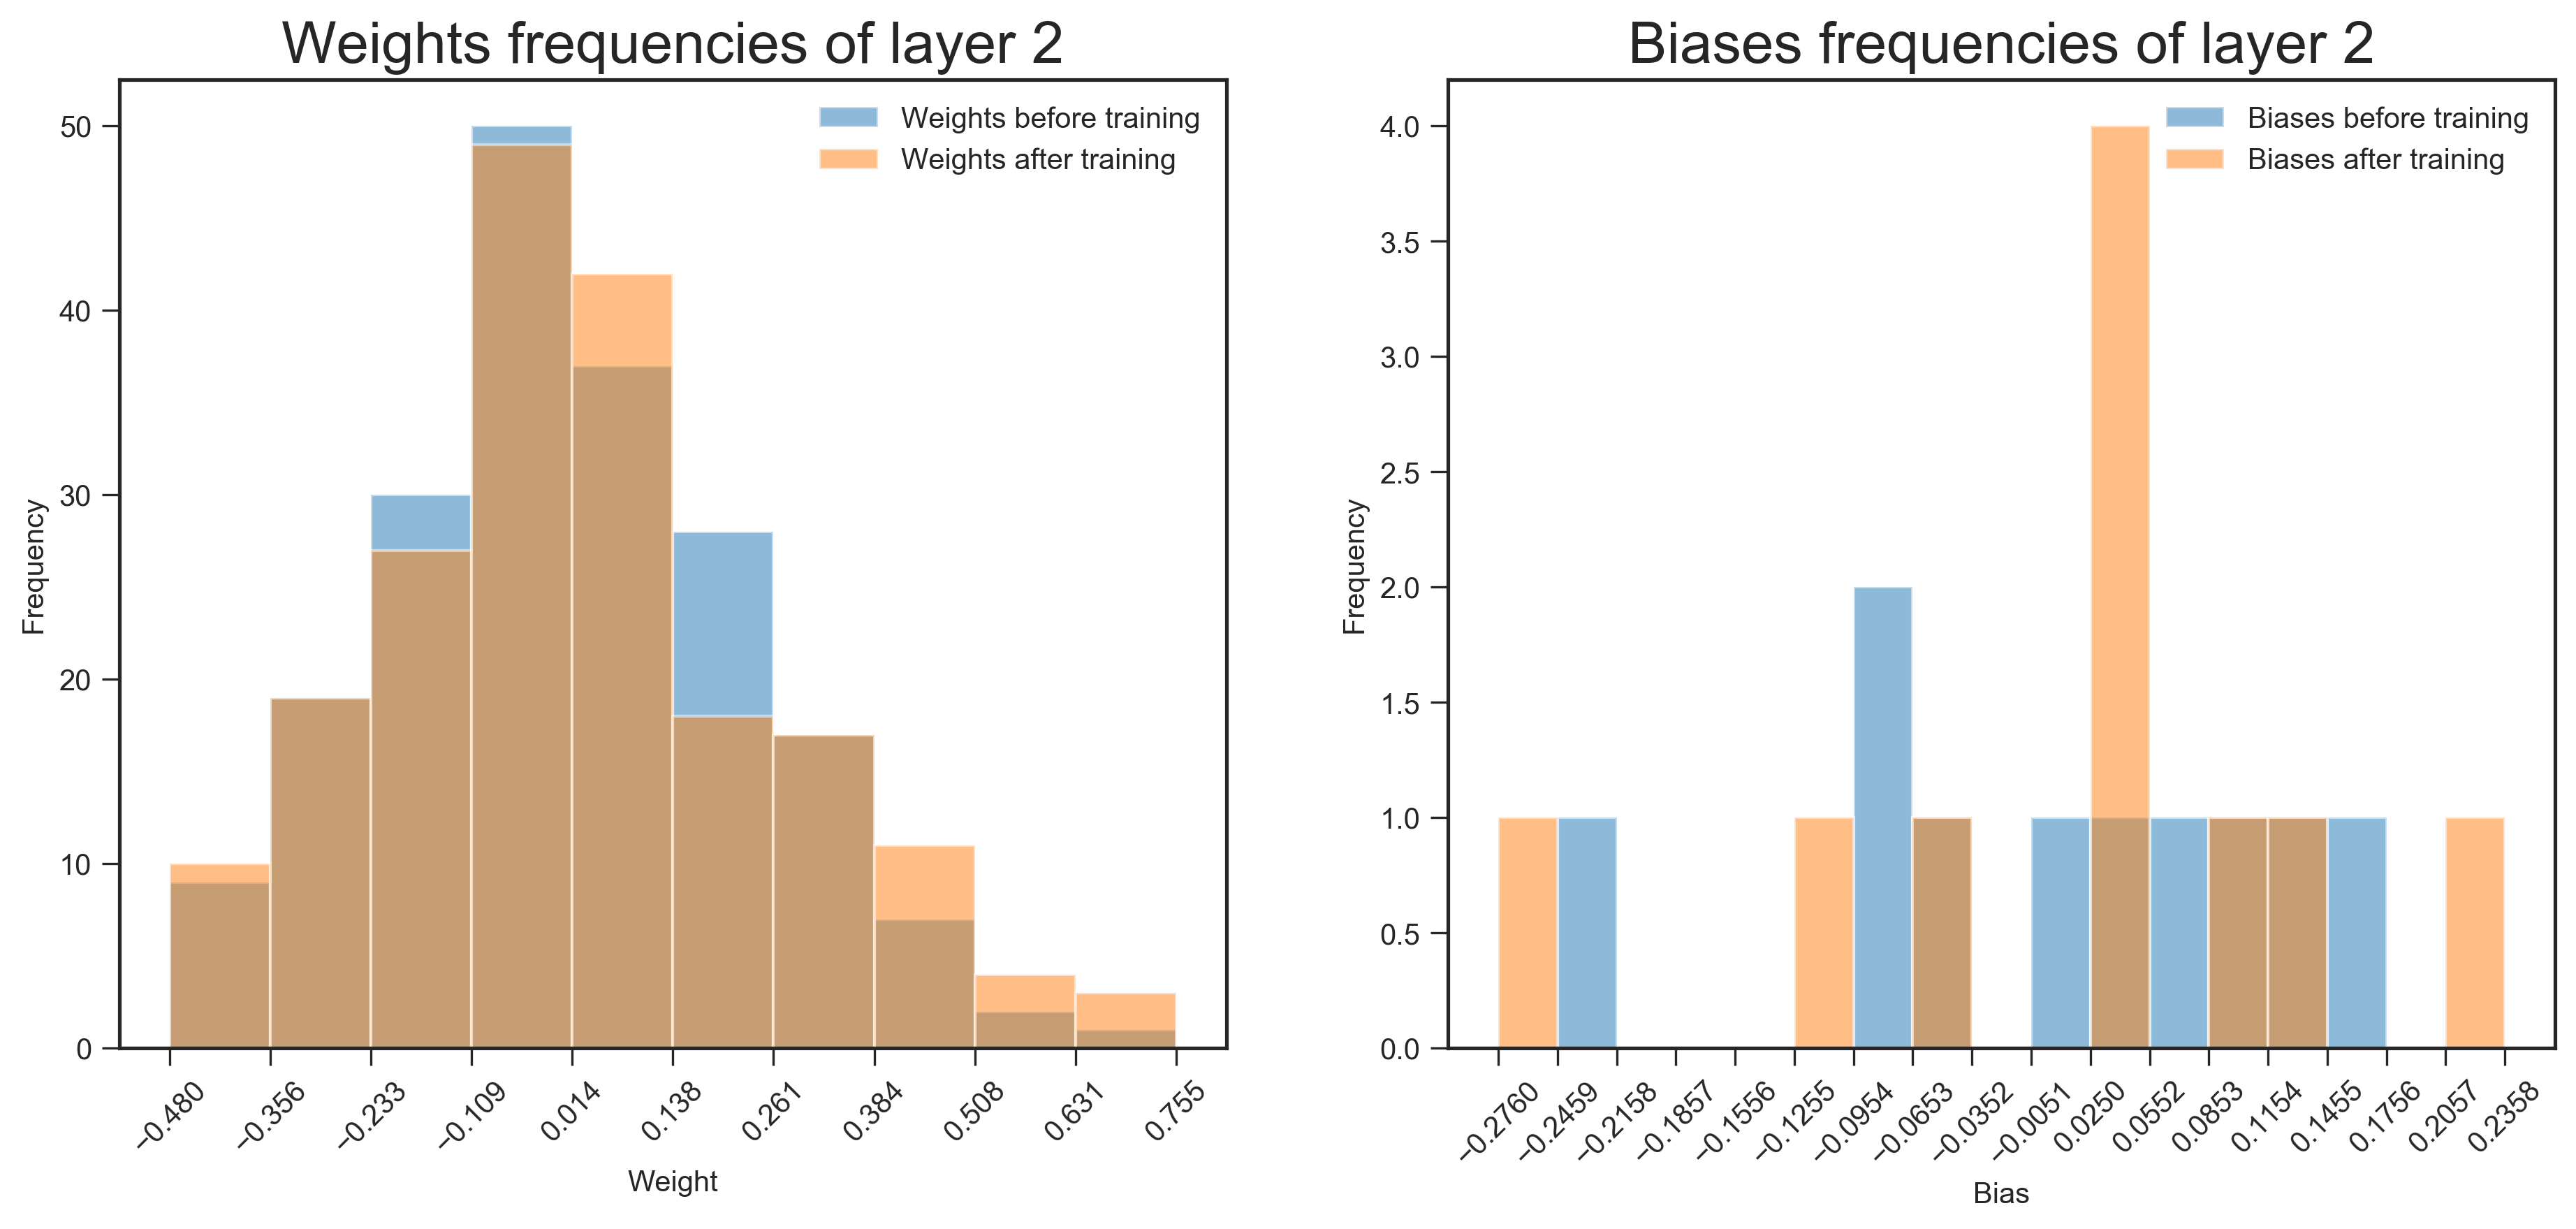
\includegraphics[width=0.9\textwidth]{immagini/clus_hist_L2.png}%
	}\par\medskip        
	\subcaptionbox{Third layer\label{fig:clus_hist_L3}}{%
		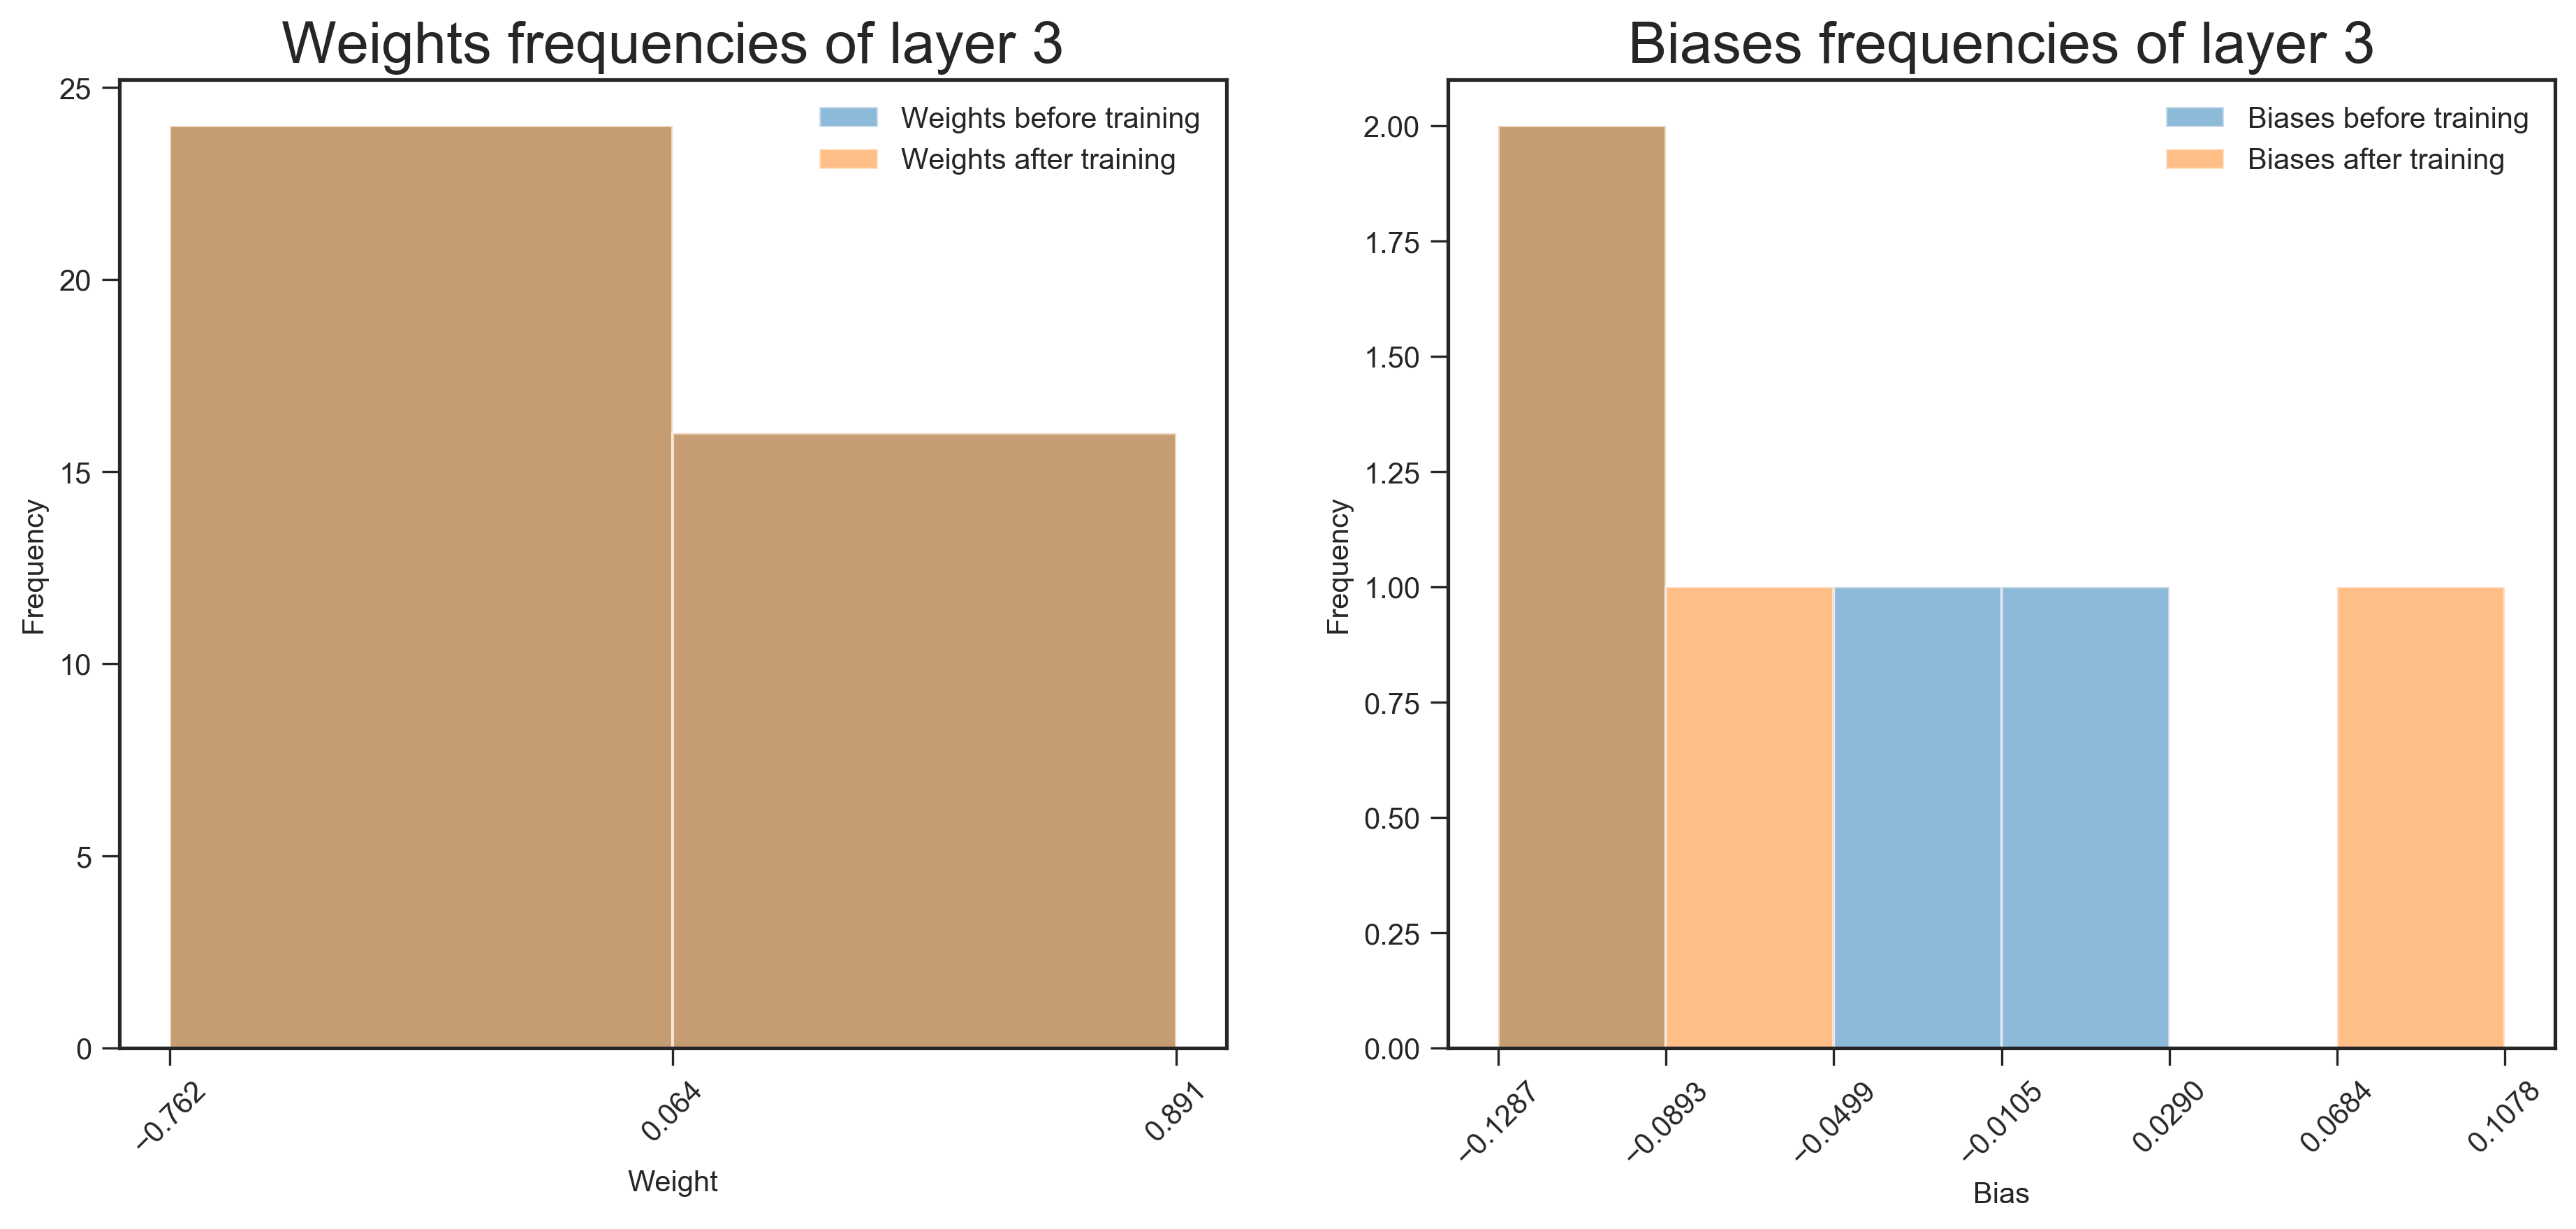
\includegraphics[width=0.9\textwidth]{immagini/clus_hist_L3.png}%
	}
	\caption{Frequency plots of the parameters before and after training. Clusters data set.}
	\label{fig:clus_hist}
\end{figure}
%\newpage
\begin{figure}[h!]
	\centering
	\subcaptionbox{First layer\label{fig:clus_kde_L1}}{%
		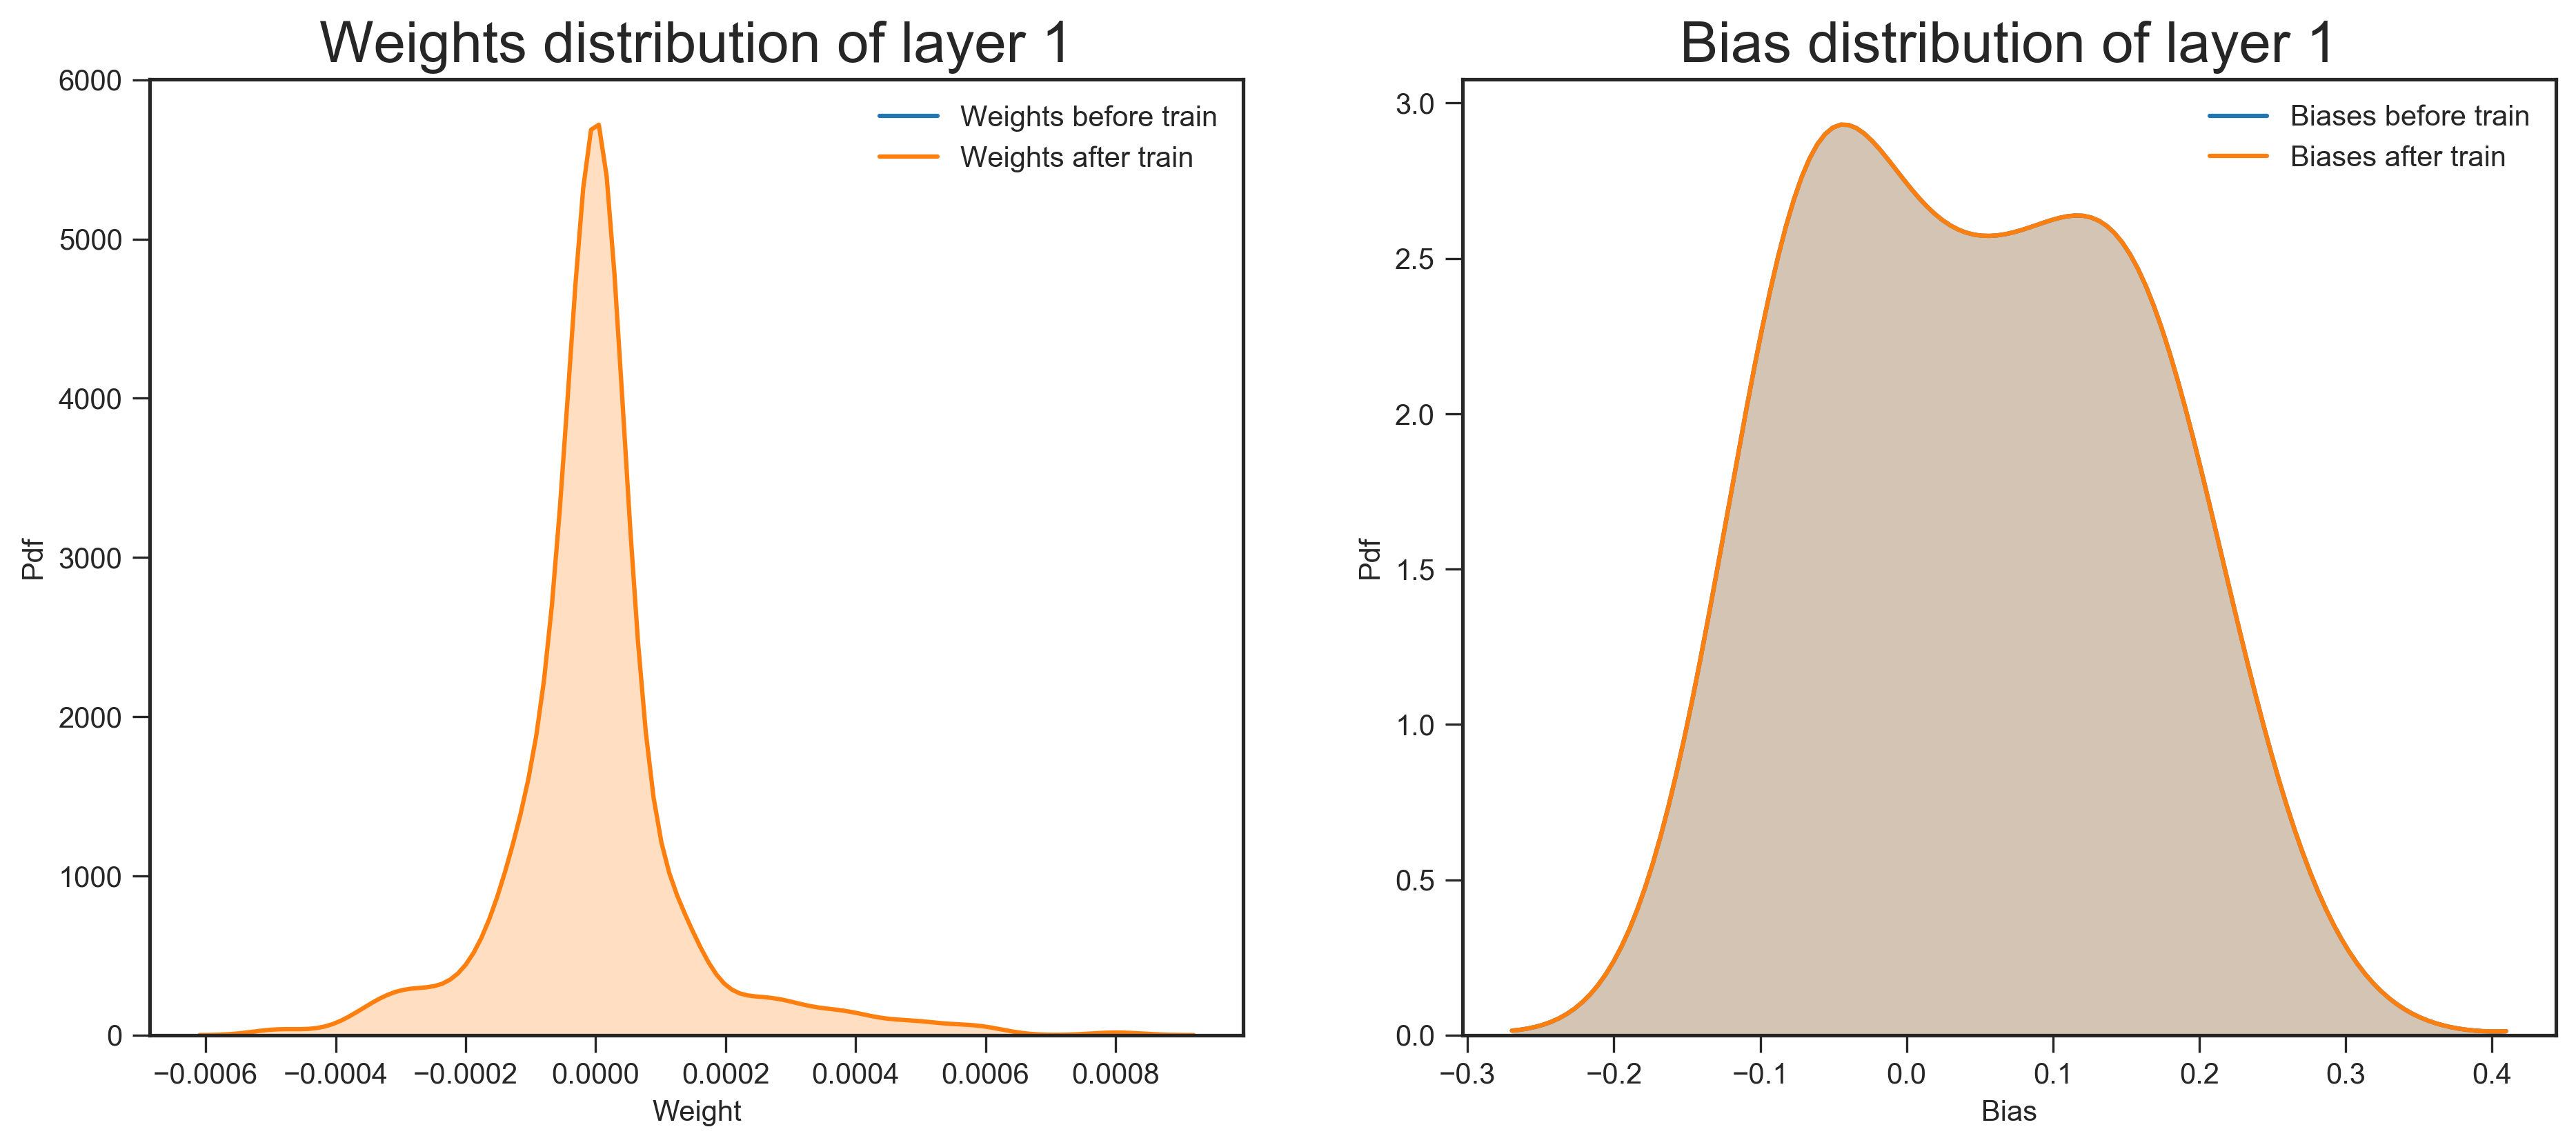
\includegraphics[width=0.9\textwidth]{immagini/clus_kde_L1.png}%
	}\par\medskip
	\subcaptionbox{Second layer\label{fig:clus_kde_L2}}{%
		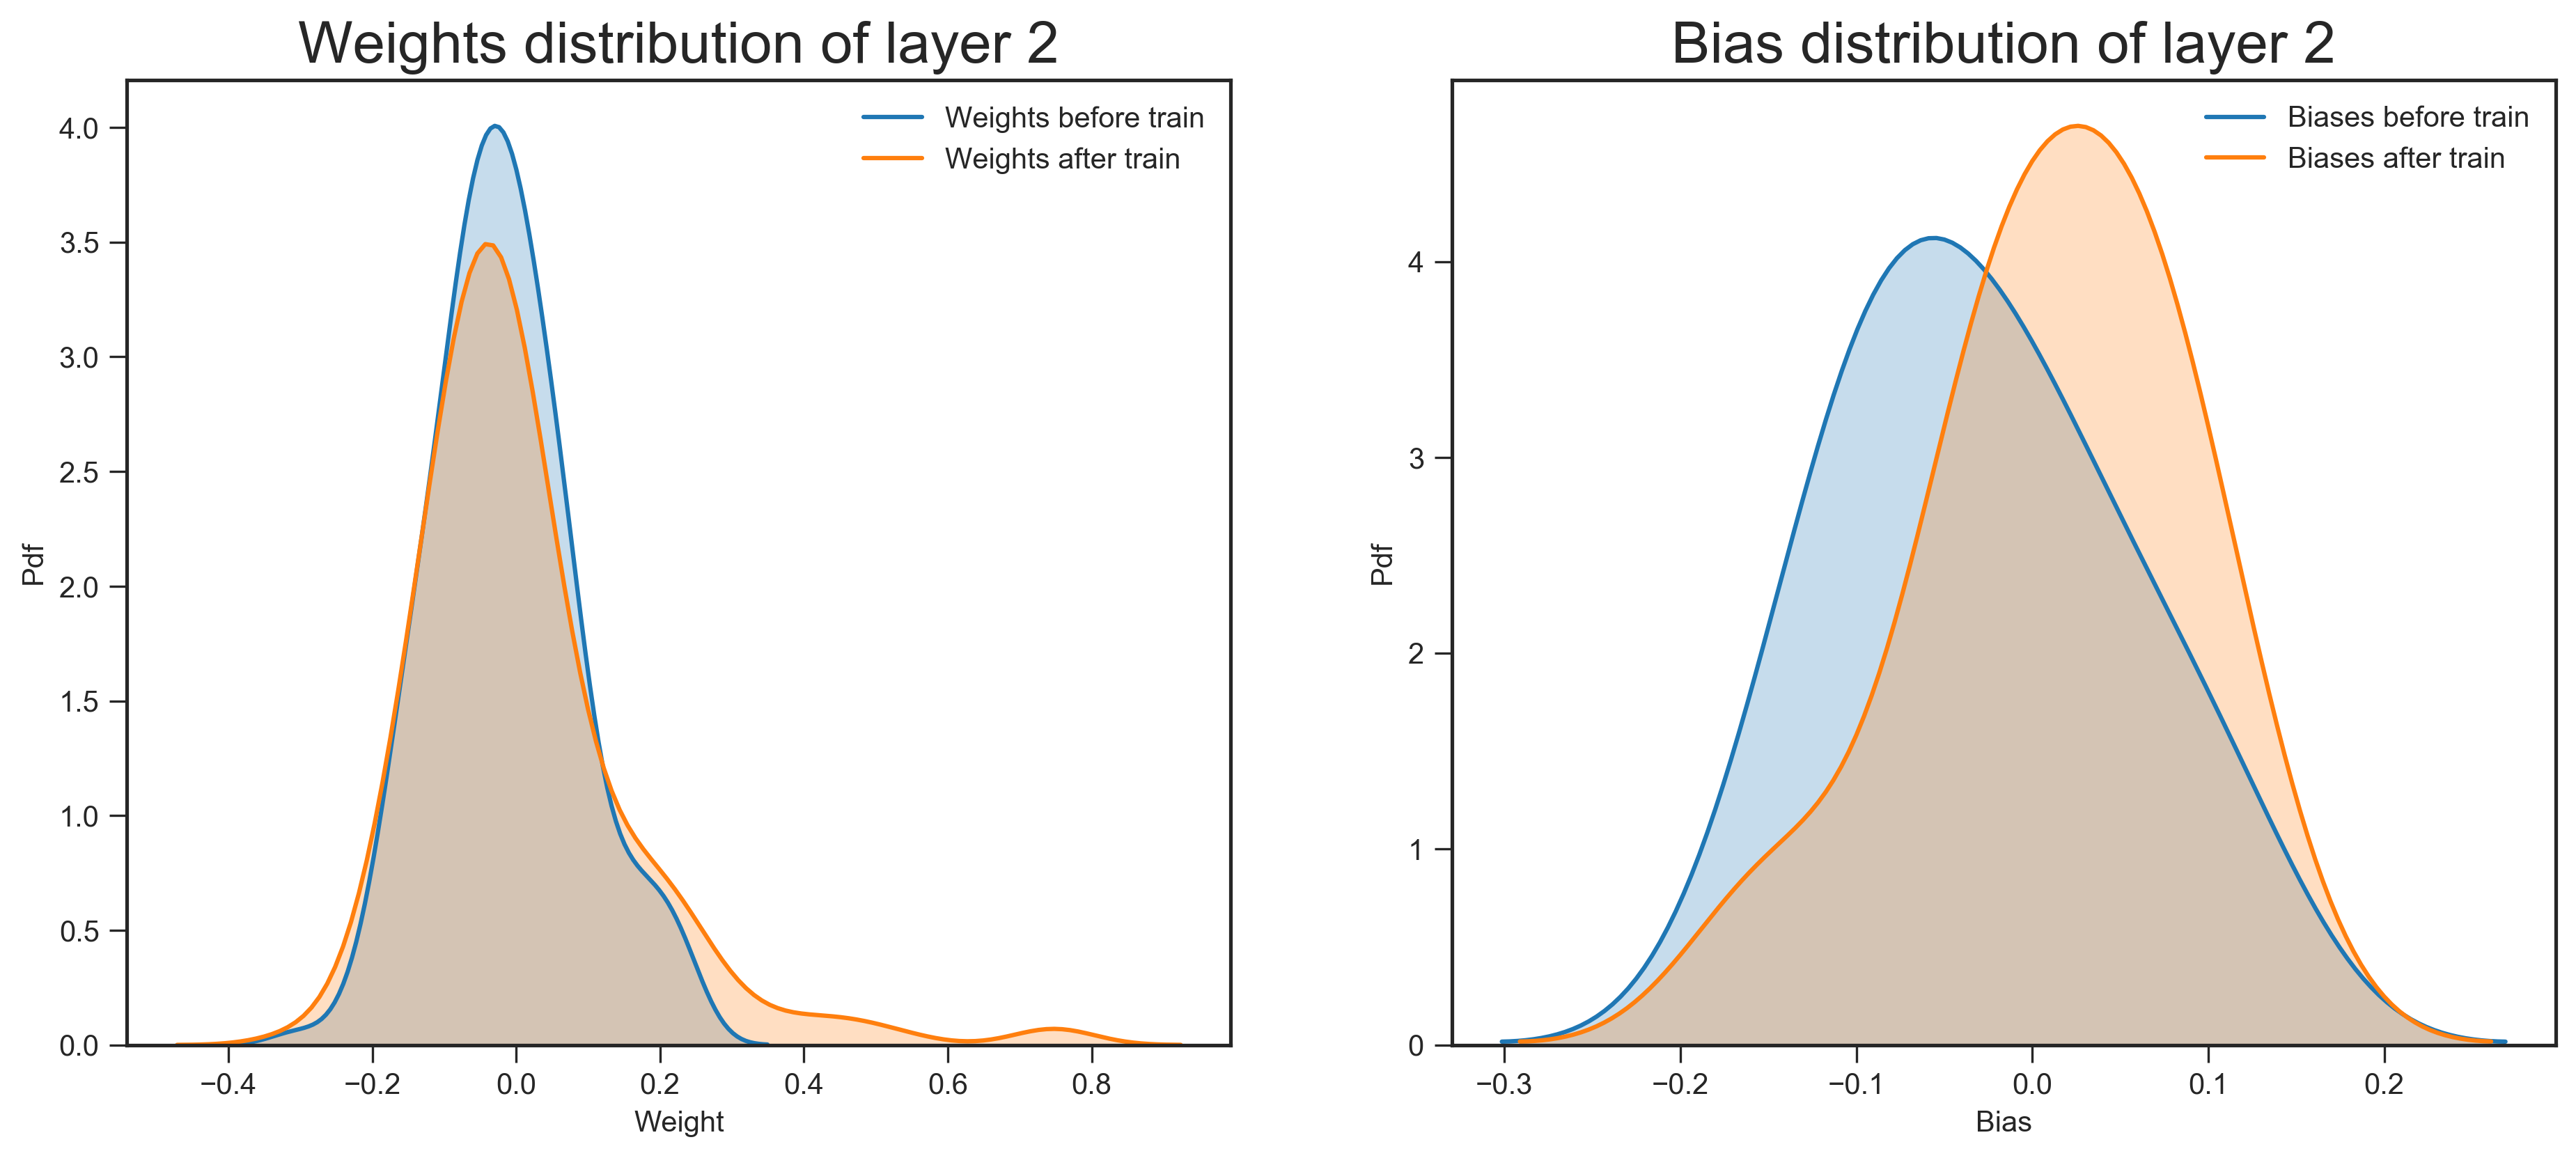
\includegraphics[width=0.9\textwidth]{immagini/clus_kde_L2.png}%
	}\par\medskip        
	\subcaptionbox{Third layer\label{fig:clus_kde_L3}}{%
		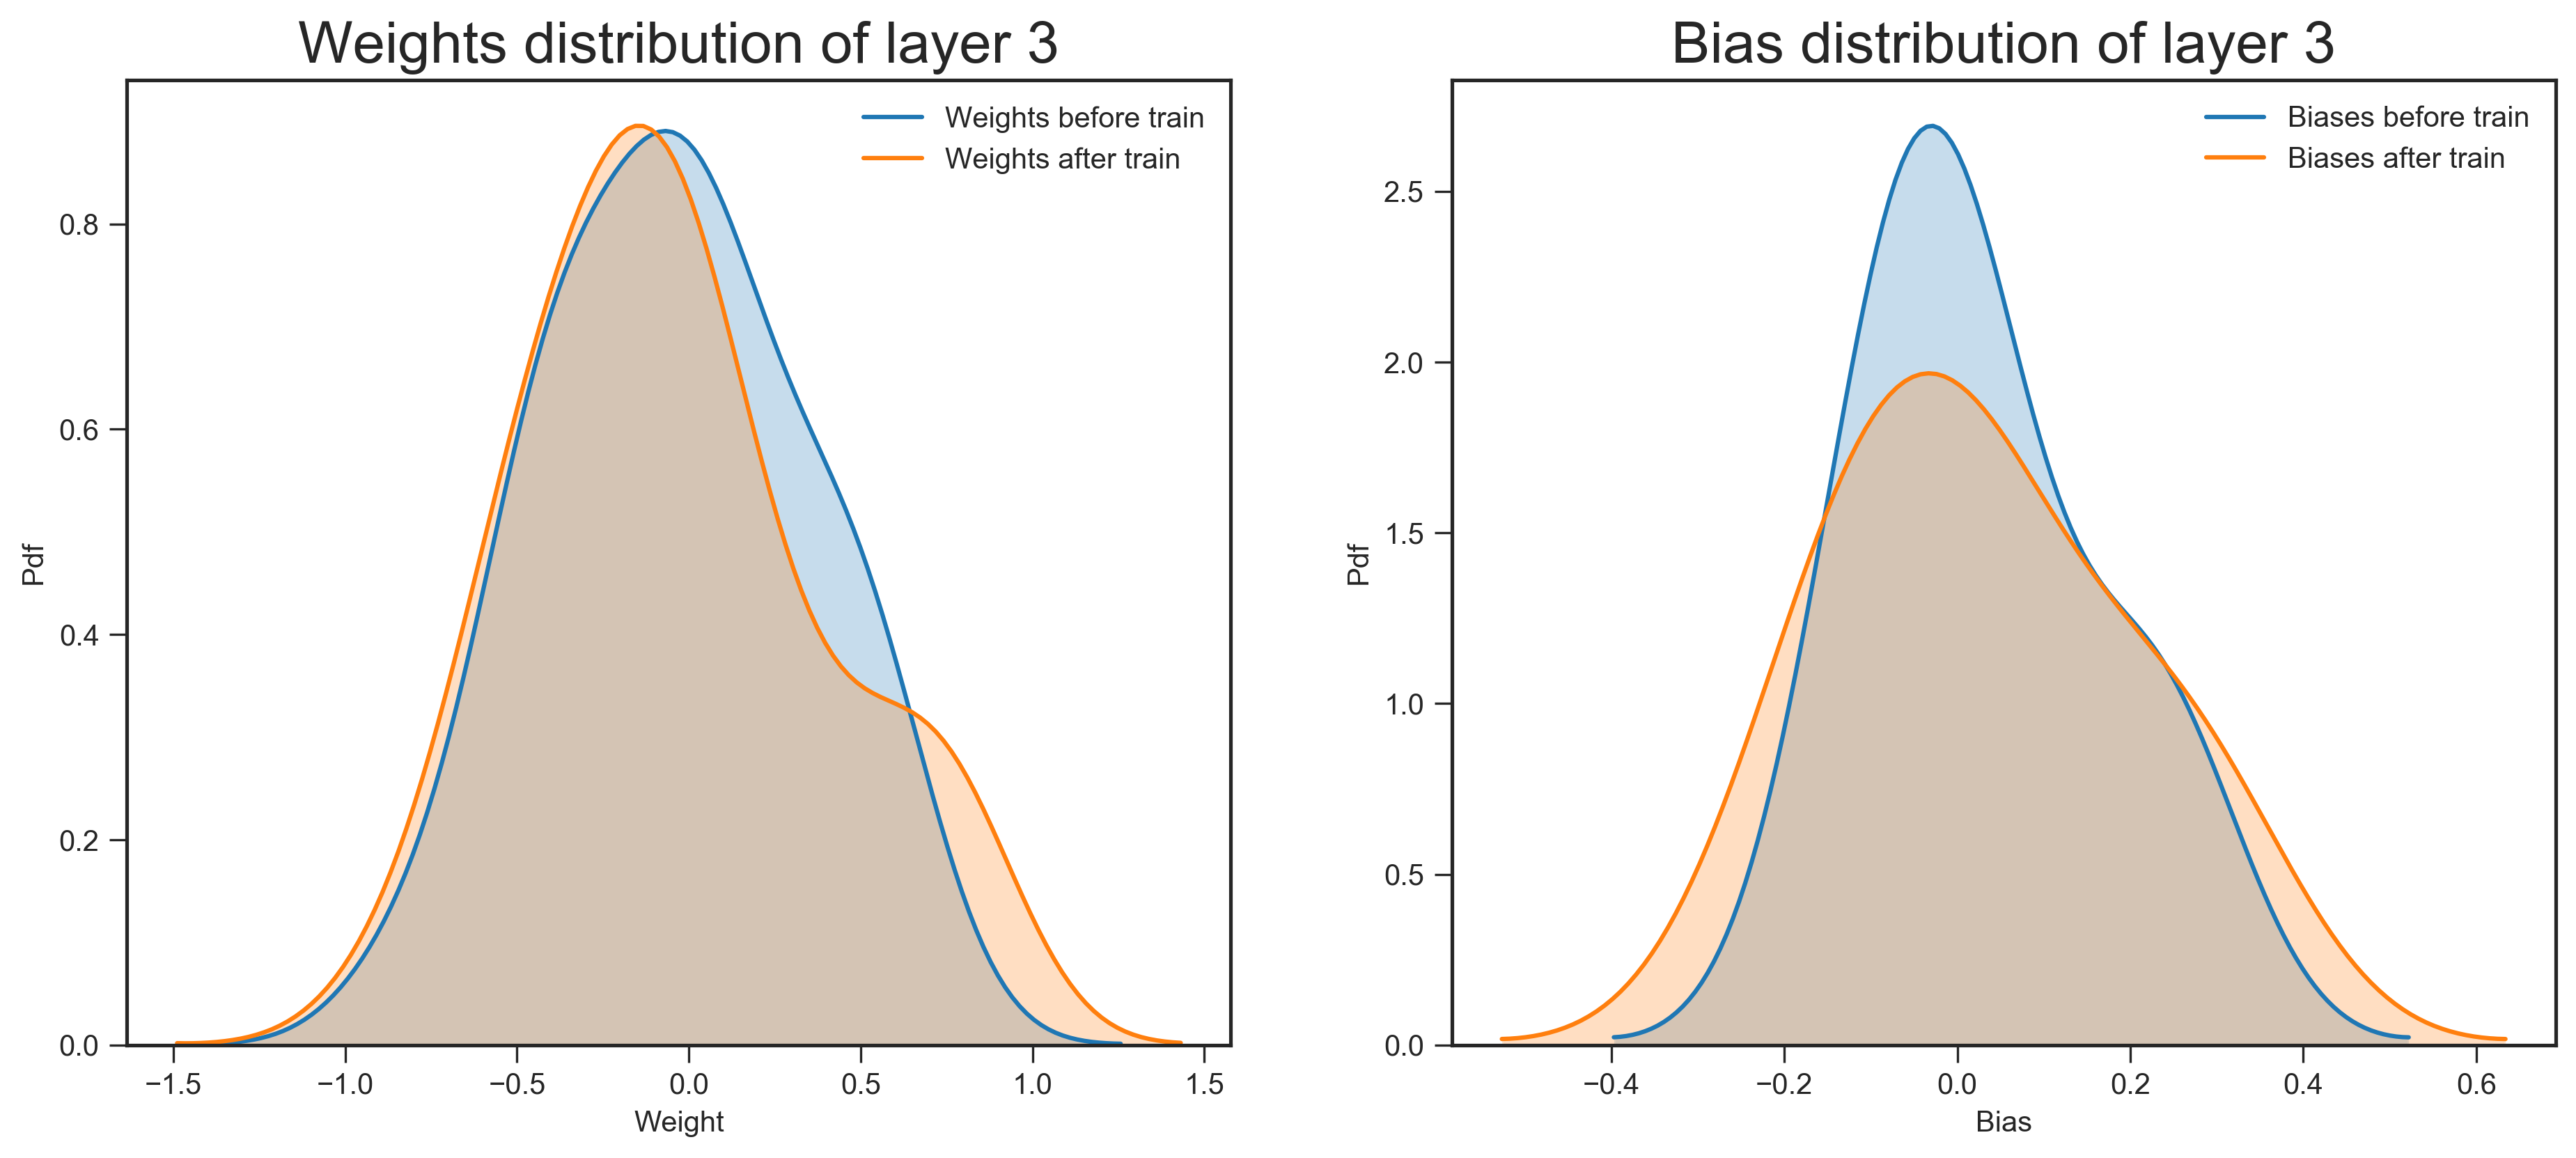
\includegraphics[width=0.9\textwidth]{immagini/clus_kde_L3.png}%
	}
	\caption{KDE plots of the parameters before and after training. Clusters data set.}
	\label{fig:clus_kde}
\end{figure}

\begin{figure}[h!]
	\centering
	\subcaptionbox{First layer\label{fig:mvg_hist_L1}}{%
		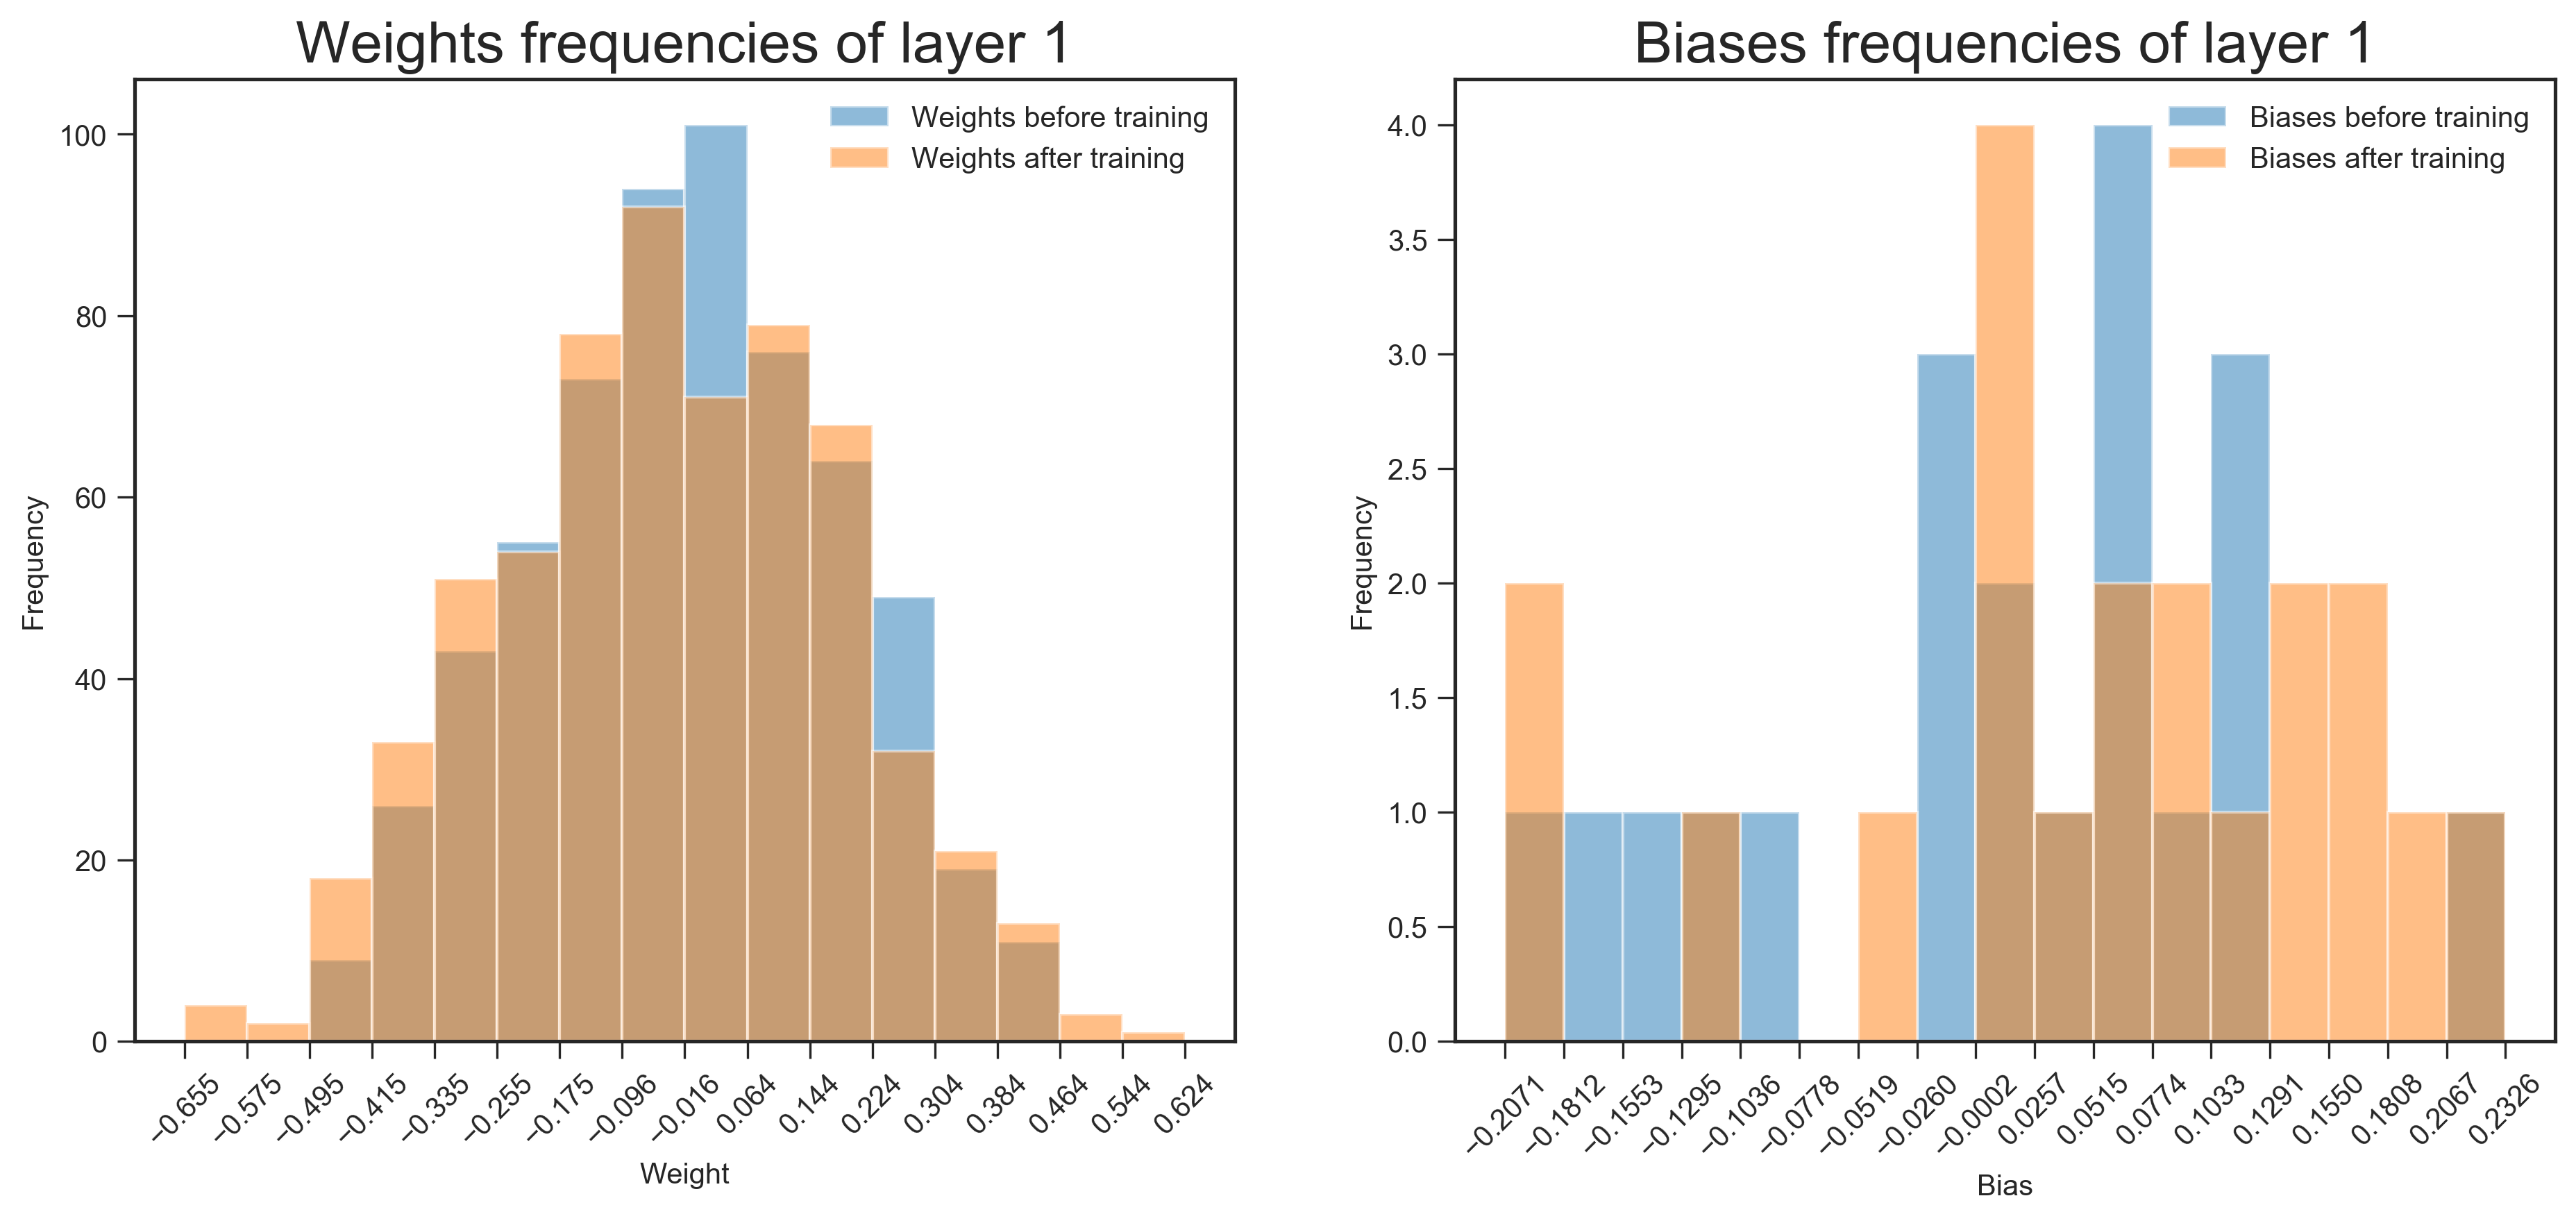
\includegraphics[width=0.9\textwidth]{immagini/mvg_hist_L1.png}%
	}\par\medskip
	\subcaptionbox{Second layer\label{fig:mvg_hist_L2}}{%
		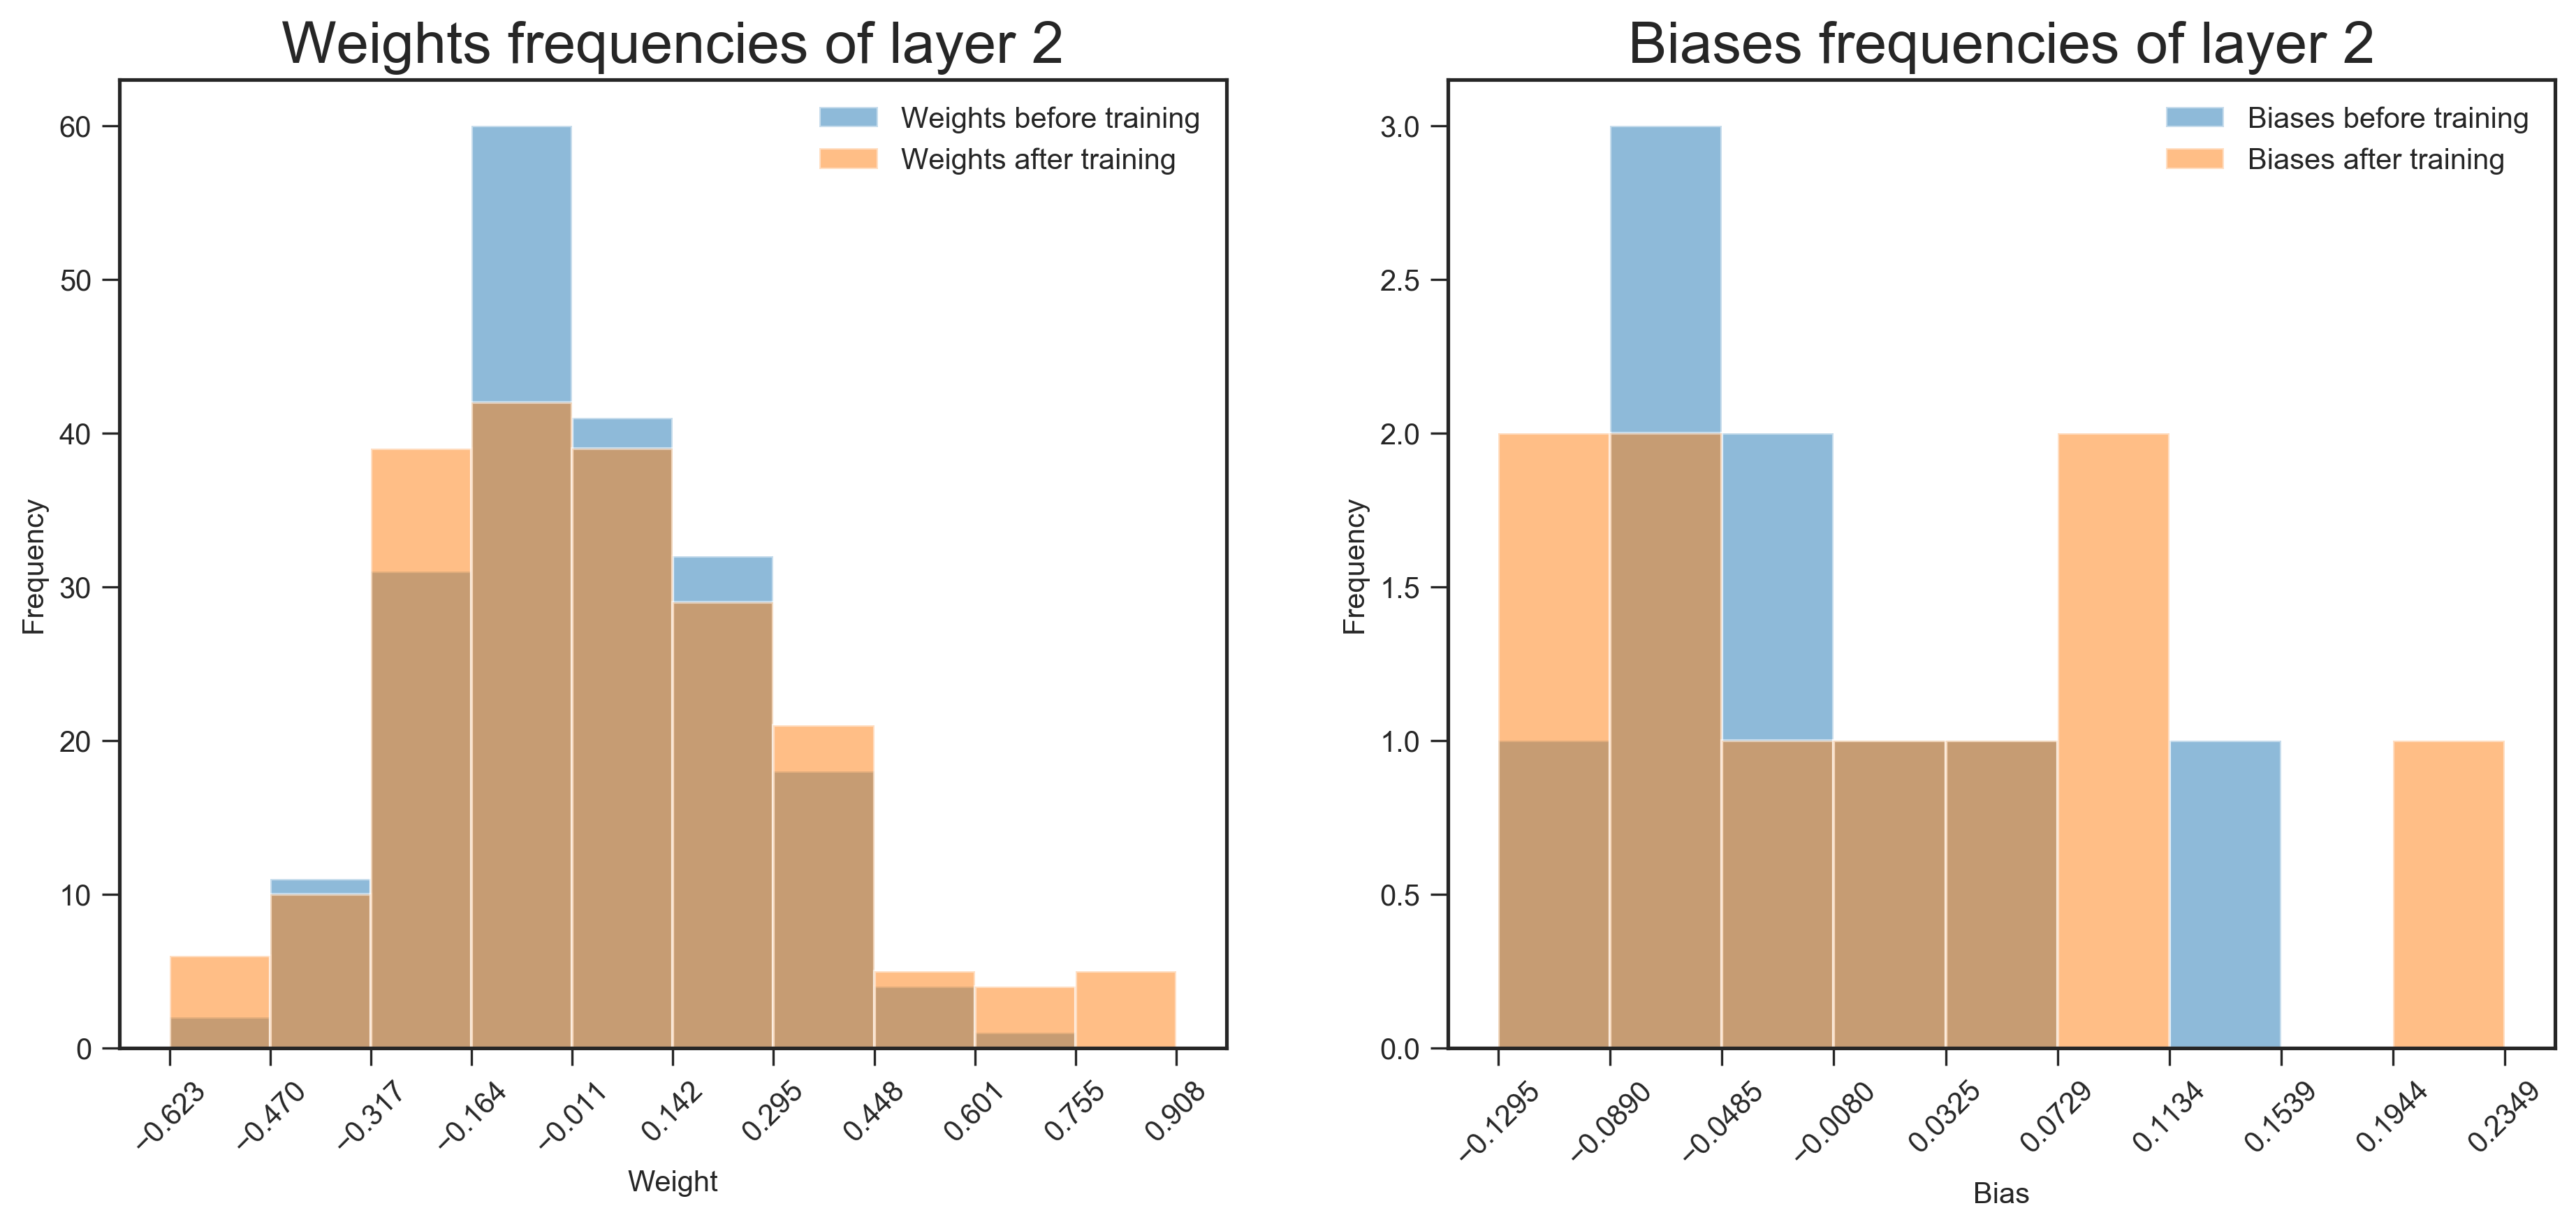
\includegraphics[width=0.9\textwidth]{immagini/mvg_hist_L2.png}%
	}\par\medskip        
	\subcaptionbox{Third layer\label{fig:mvg_hist_L3}}{%
		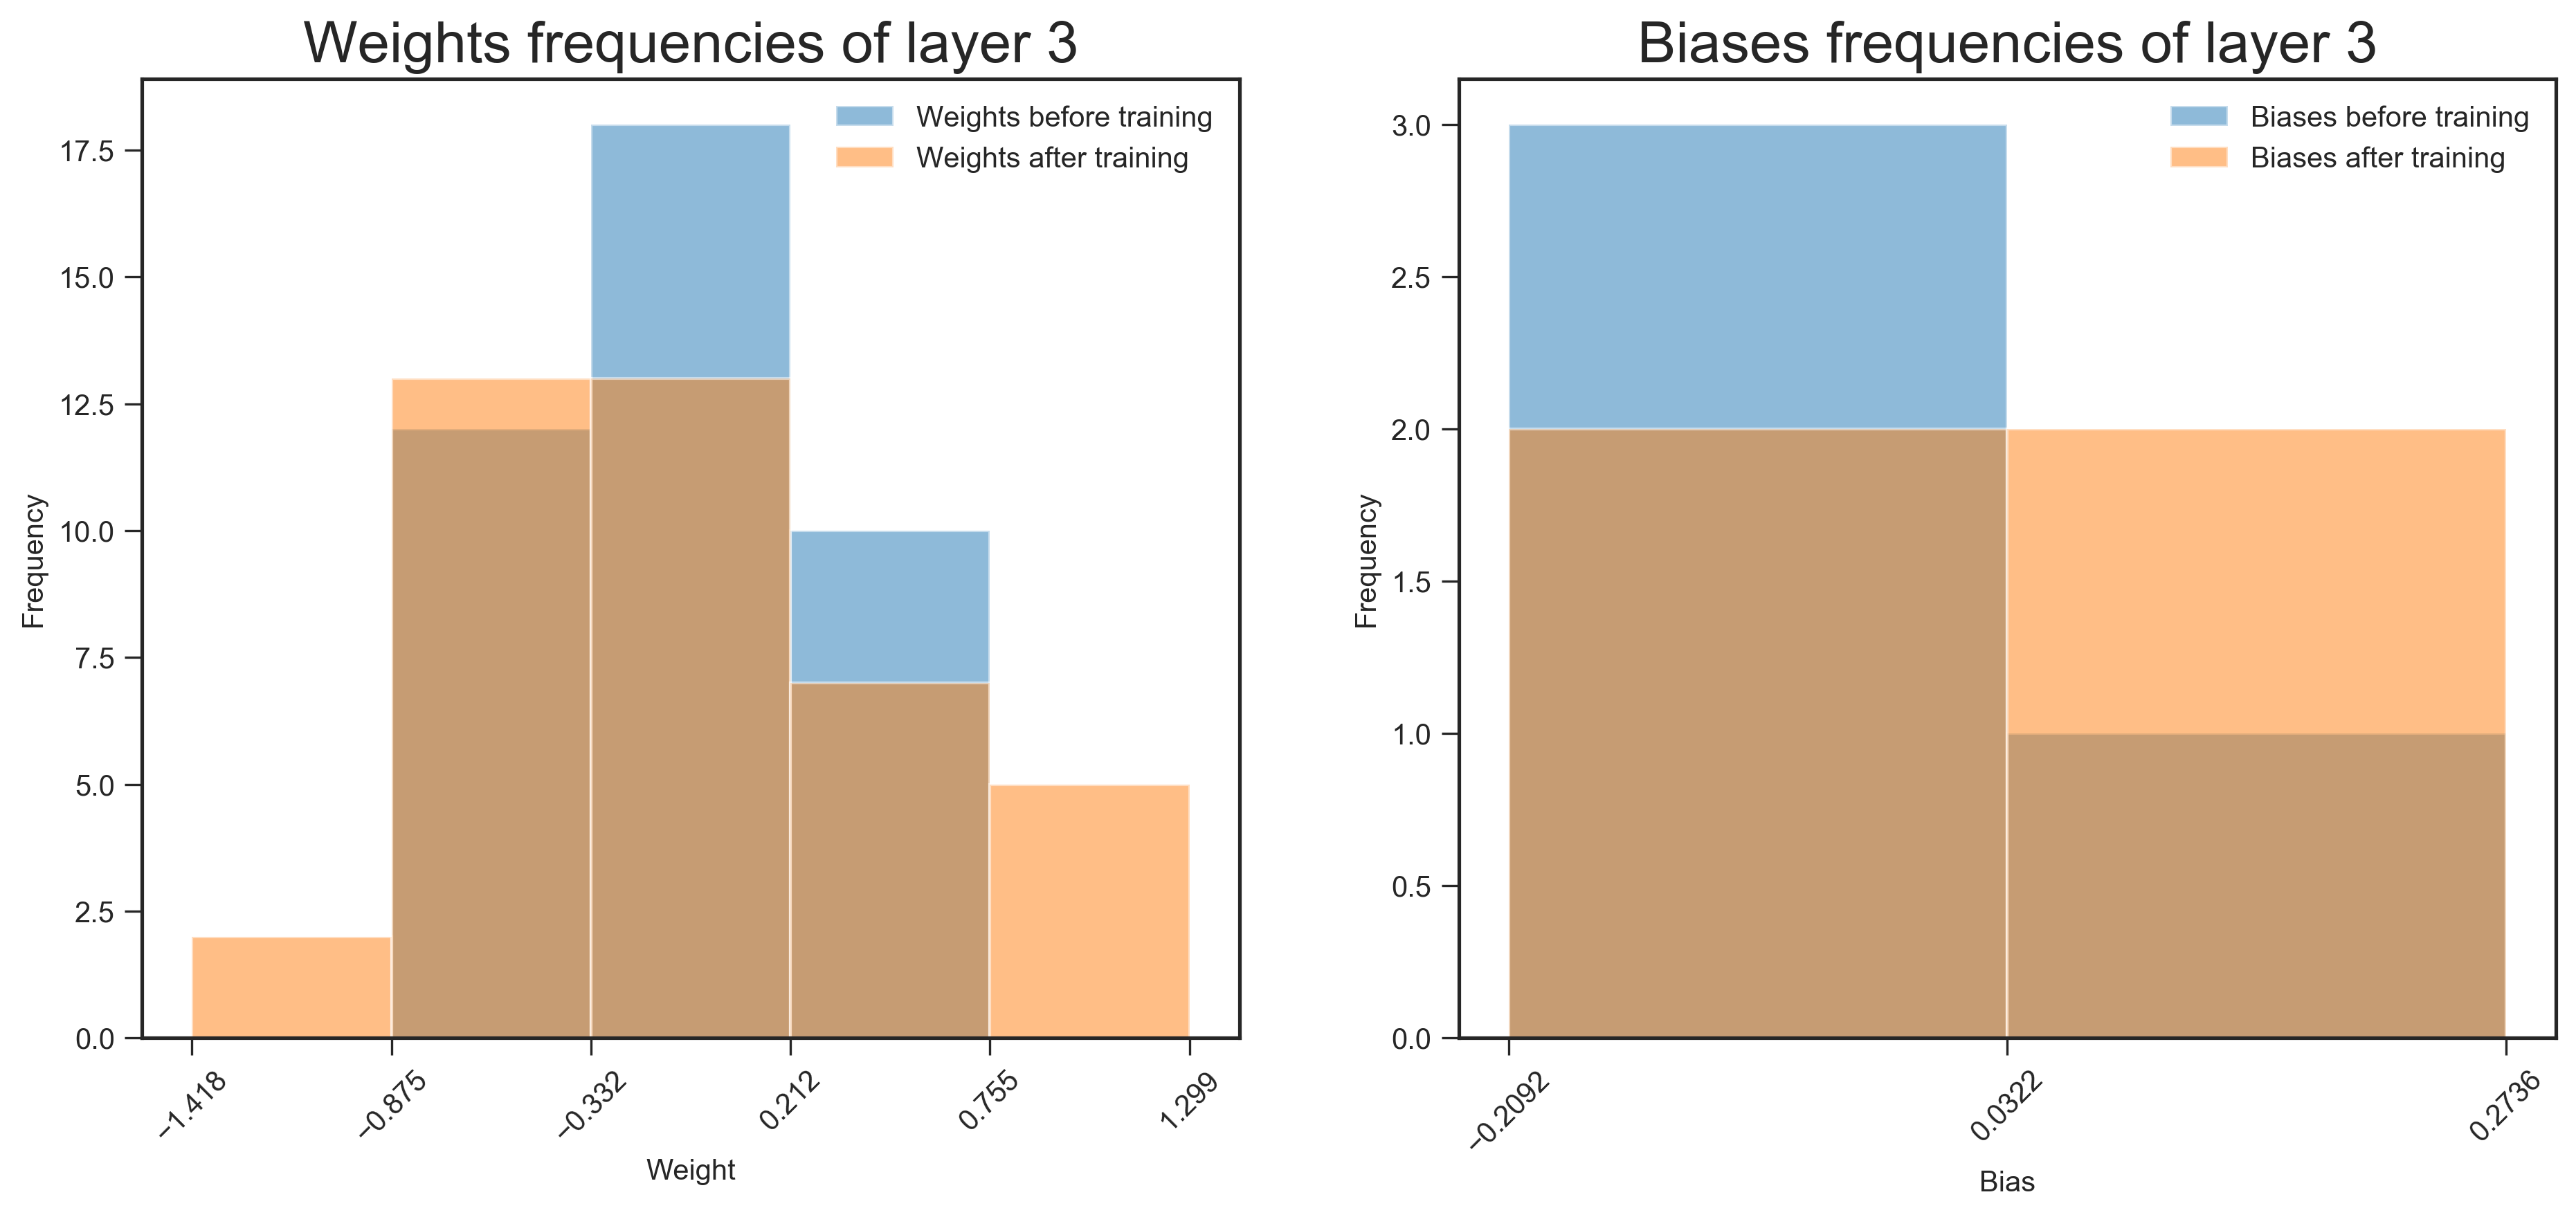
\includegraphics[width=0.9\textwidth]{immagini/mvg_hist_L3.png}%
	}
	\caption{Frequency plots of the parameters before and after training. MVG.}
	\label{fig:mvg_hist}
\end{figure}
%\newpage
\begin{figure}[h!]
	\centering
	\subcaptionbox{First layer\label{fig:mvg_kde_L1}}{%
		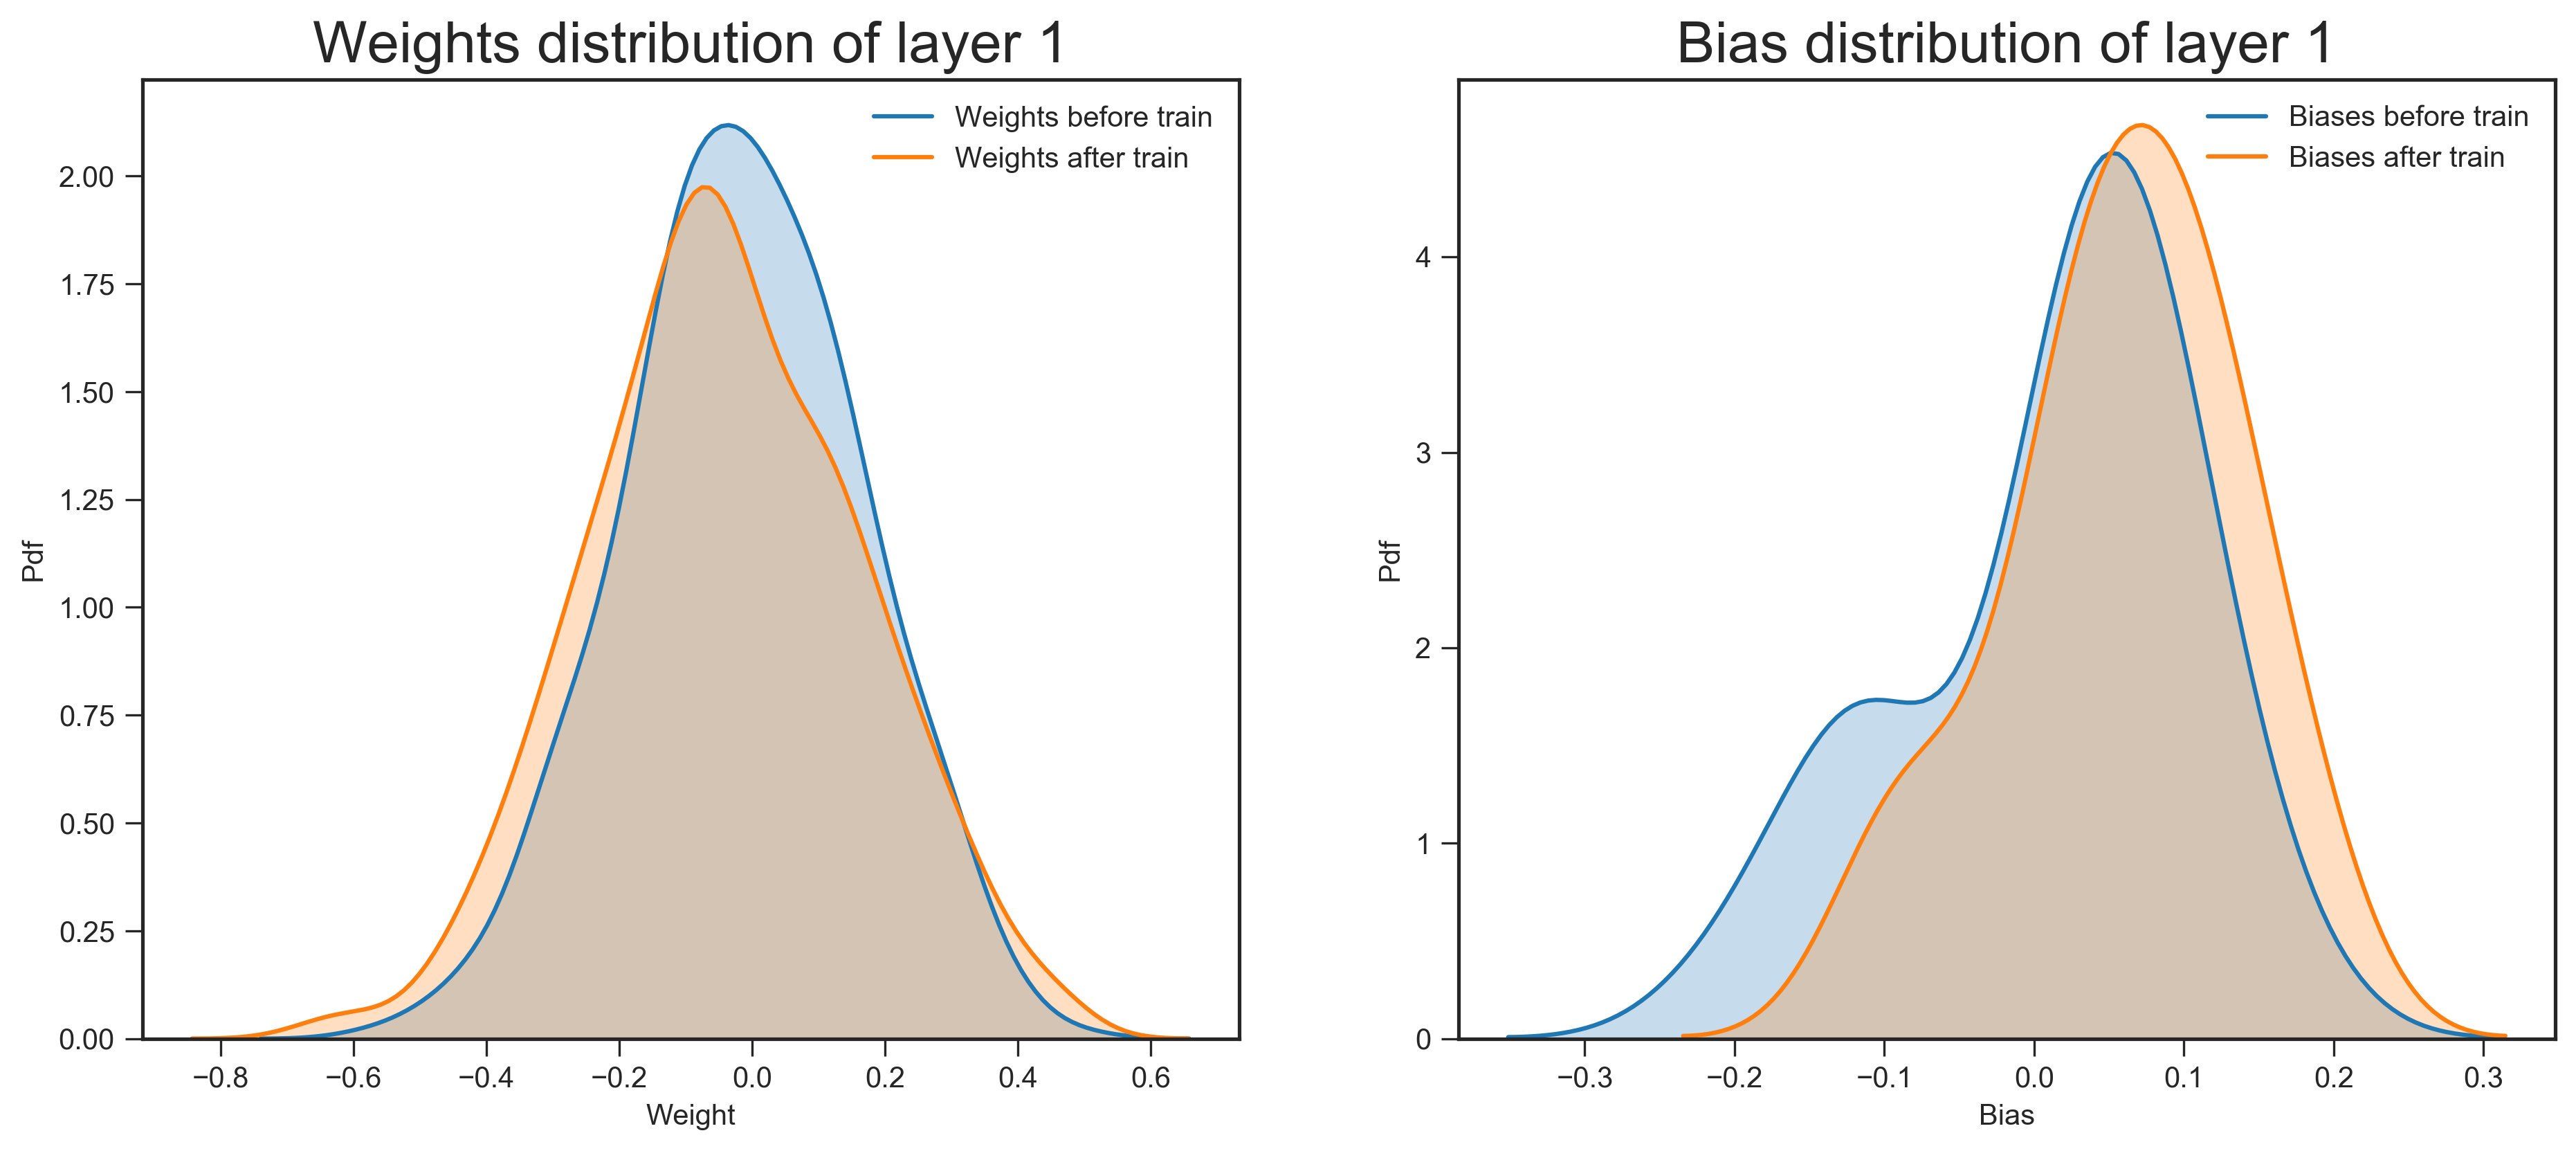
\includegraphics[width=0.9\textwidth]{immagini/mvg_kde_L1.png}%
	}\par\medskip
	\subcaptionbox{Second layer\label{fig:mvg_kde_L2}}{%
		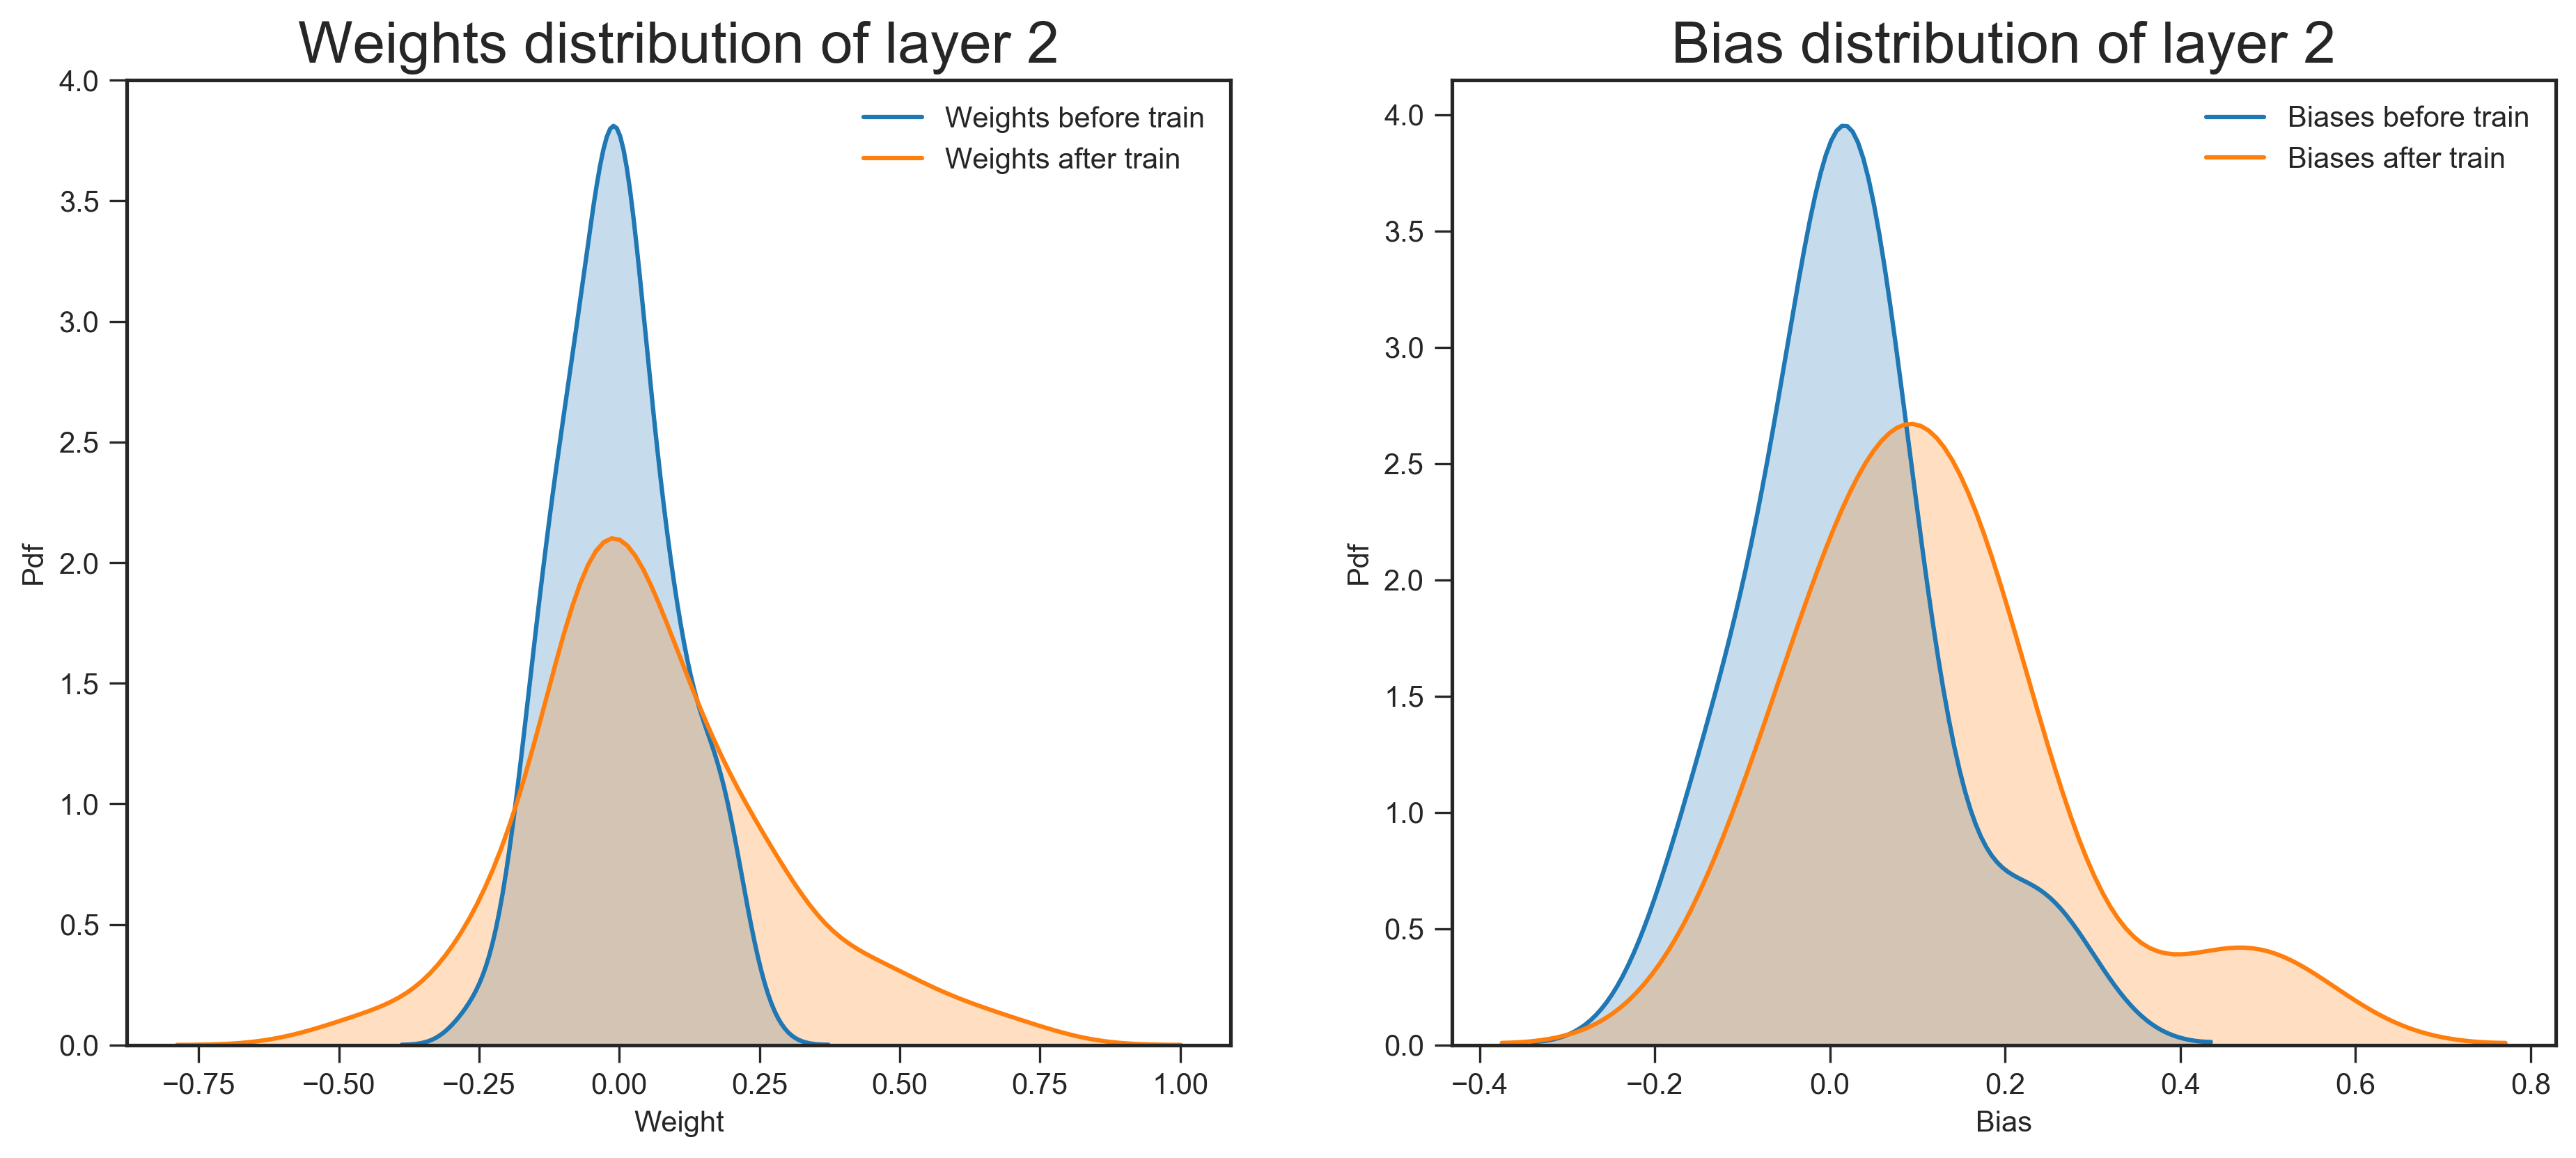
\includegraphics[width=0.9\textwidth]{immagini/mvg_kde_L2.png}%
	}\par\medskip        
	\subcaptionbox{Third layer\label{fig:mvg_kde_L3}}{%
		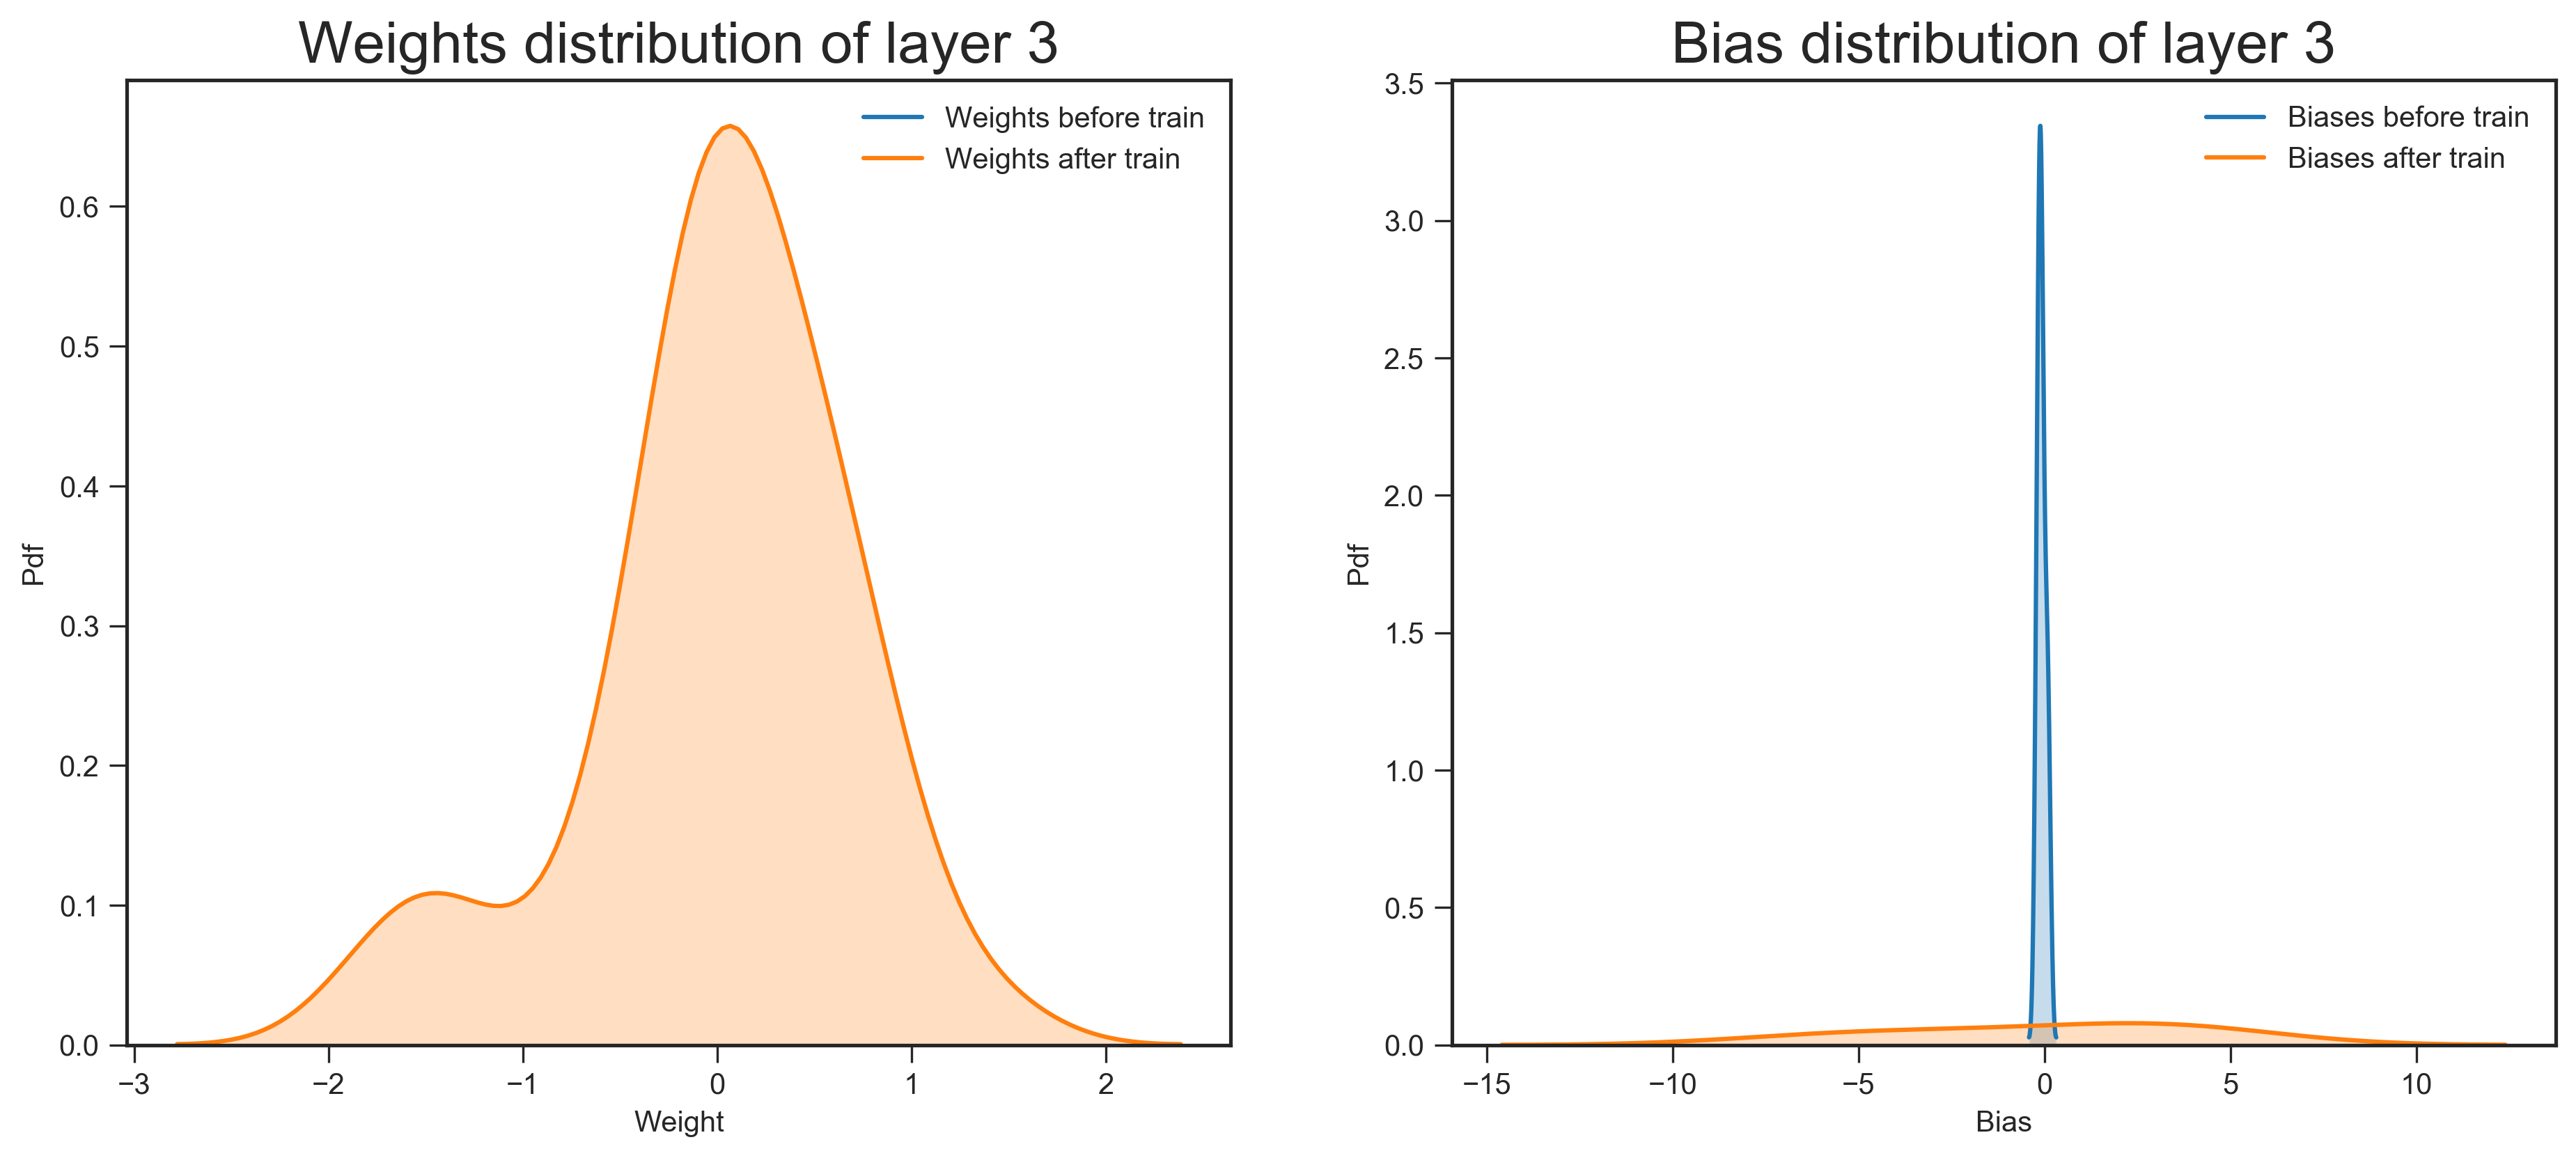
\includegraphics[width=0.9\textwidth]{immagini/mvg_kde_L3.png}%
	}
	\caption{KDE plots of the parameters before and after training. MVG.}
	\label{fig:mvg_kde}
\end{figure}


\begin{figure}[h!]
	\centering
	\subcaptionbox{Visualisation of the untrained network topological structure with connection strengths highlighted in \textcolor{red}{red} for negative valued weights and \textcolor{green}{green} for positive values ones.\label{fig:tree_net_untrained}}{%
		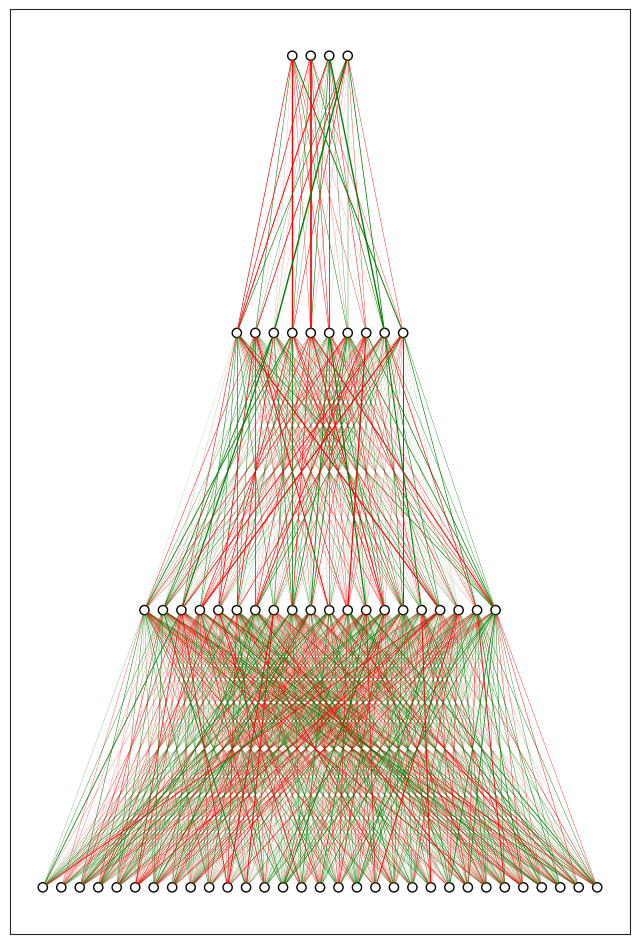
\includegraphics[width=1\textwidth]{immagini/tree_net_untrained.png}%
	}\par
	\subcaptionbox{Visualisation of the trained network topological structure with connection strengths highlighted in \textcolor{red}{red} for negative valued weights and \textcolor{green}{green} for positive values ones.\label{fig:tree_net_trained}}{%
		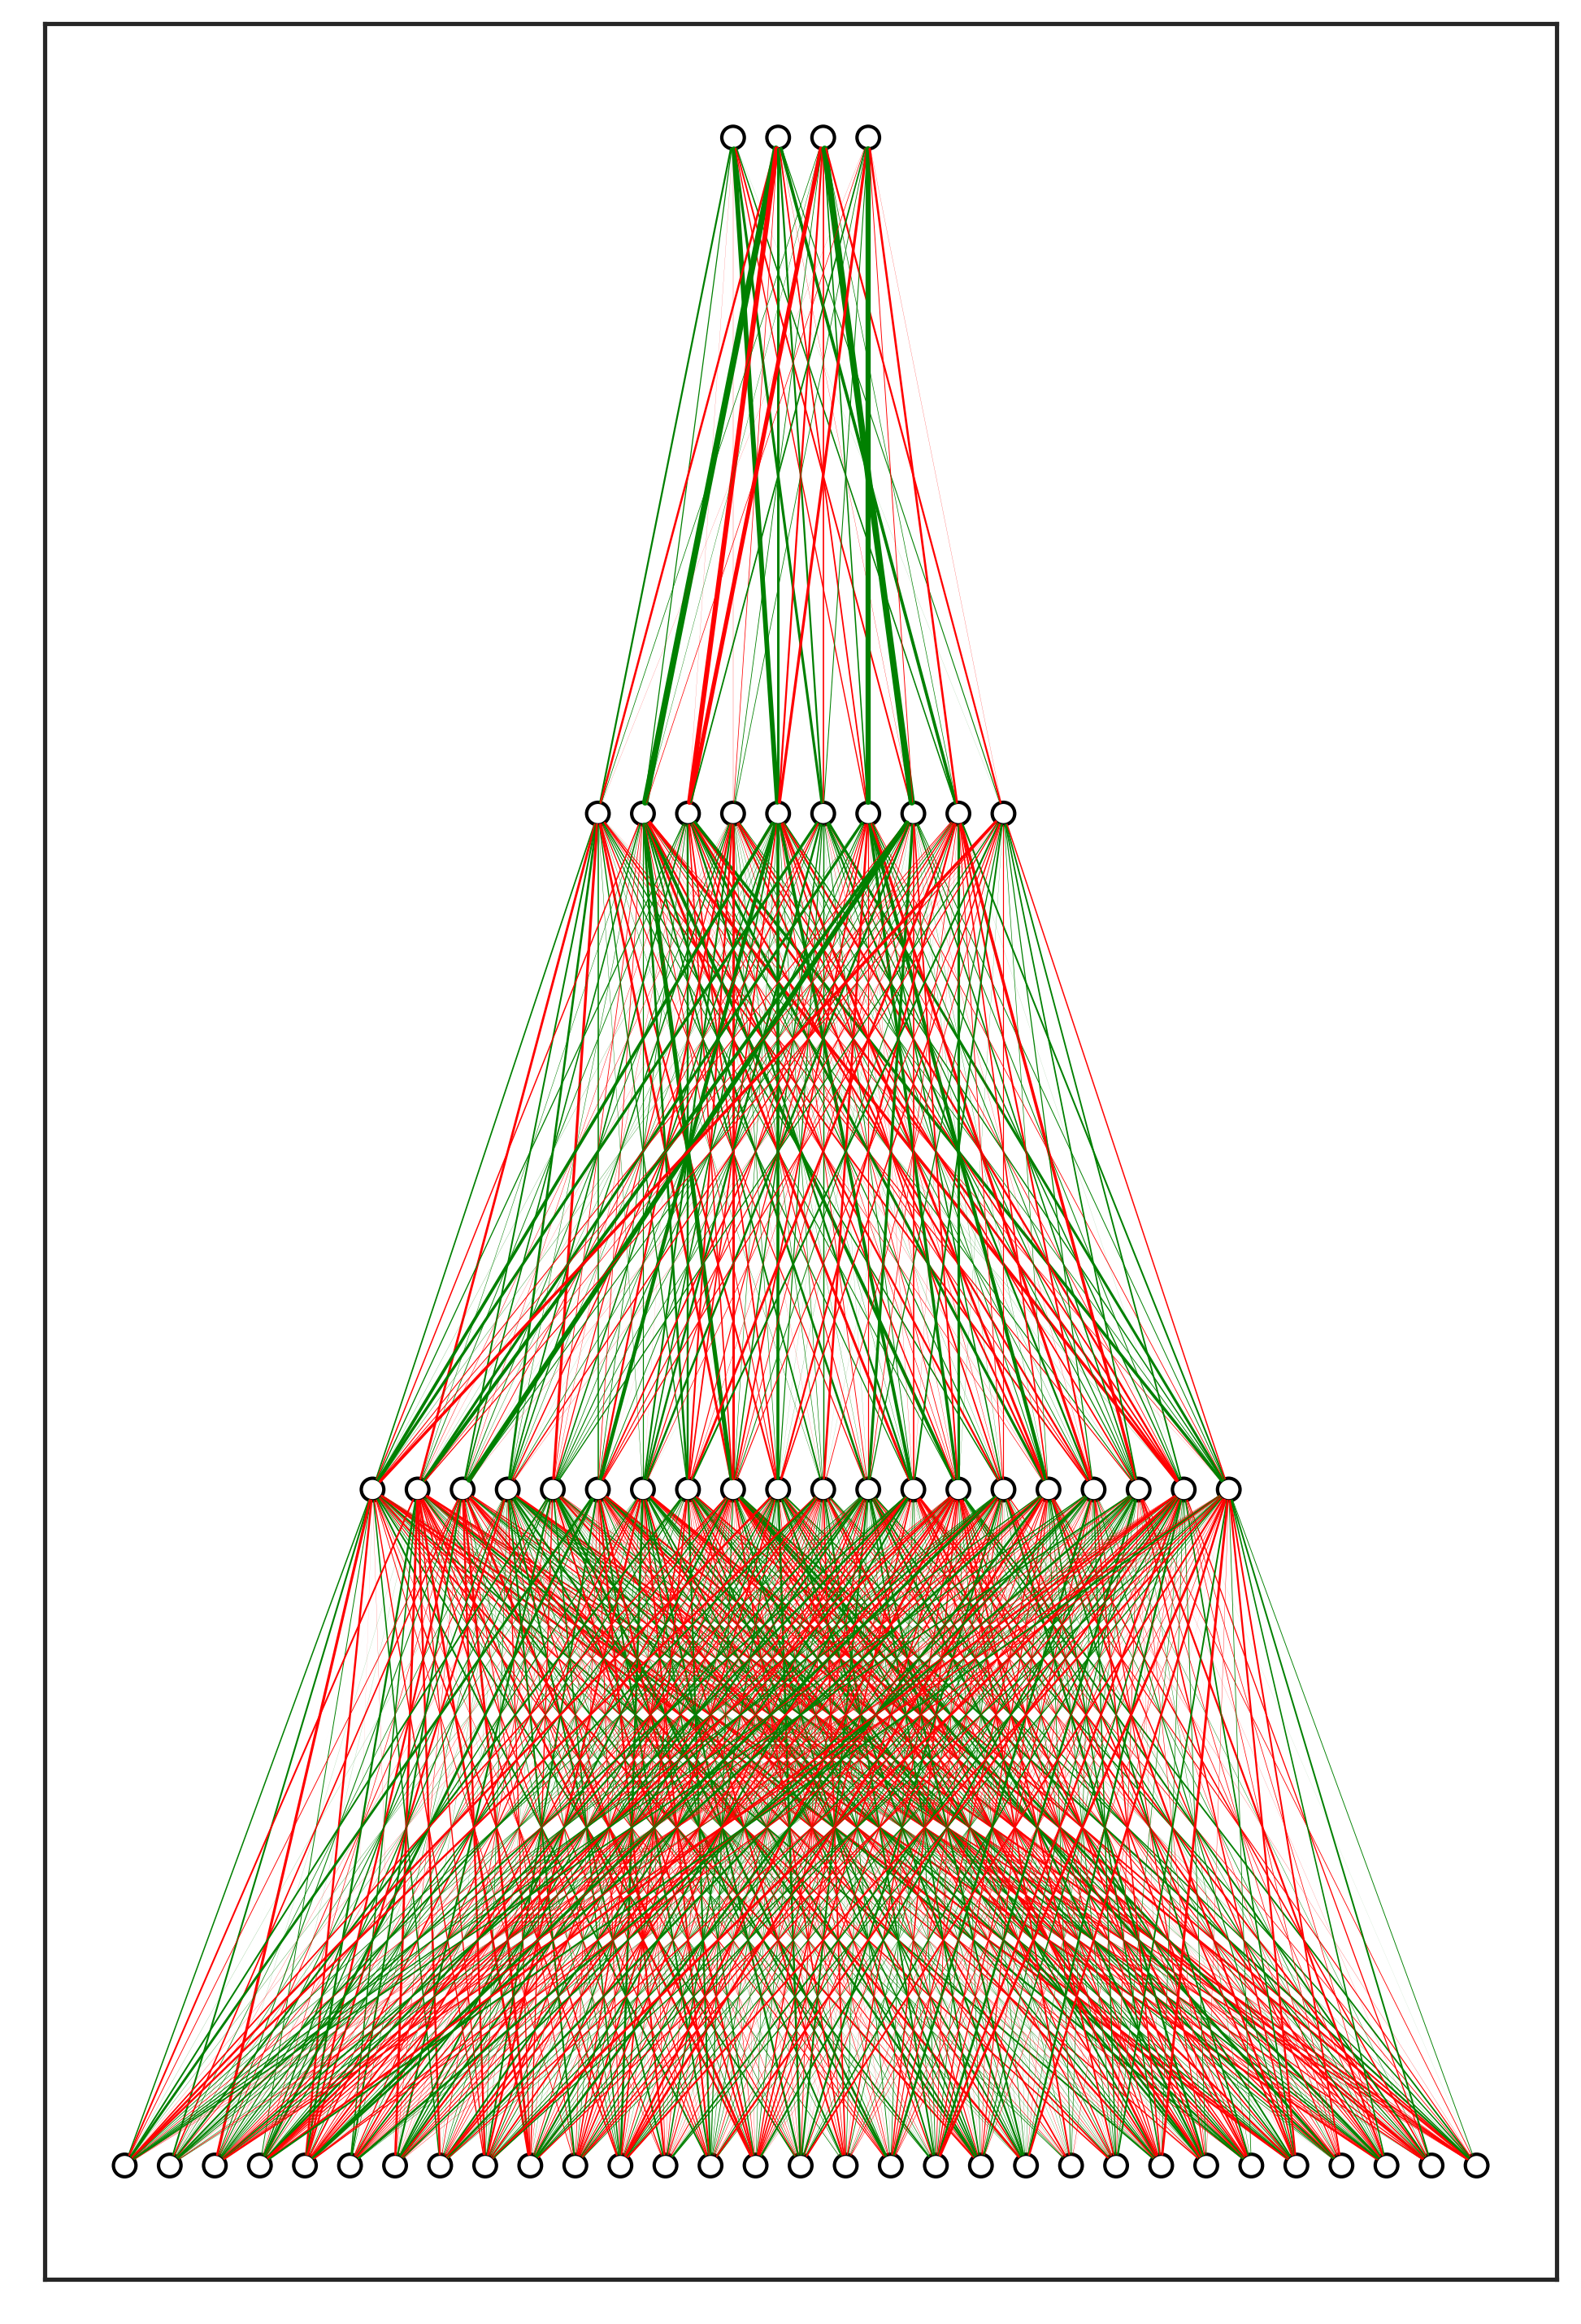
\includegraphics[width=1\textwidth]{immagini/tree_net_trained.png}%
	}
	\caption{Visualisation of the network strengths for the binary tree data set.}
	\label{fig:net_tree}
\end{figure}

\newpage
\thispagestyle{empty}

\begin{figure}[h!]
	\centering
	\subcaptionbox{Visualisation of the untrained network topological structure with connection strengths highlighted in \textcolor{red}{red} for negative valued weights and \textcolor{green}{green} for positive values ones.\label{fig:clus_net_untrained}}{%
		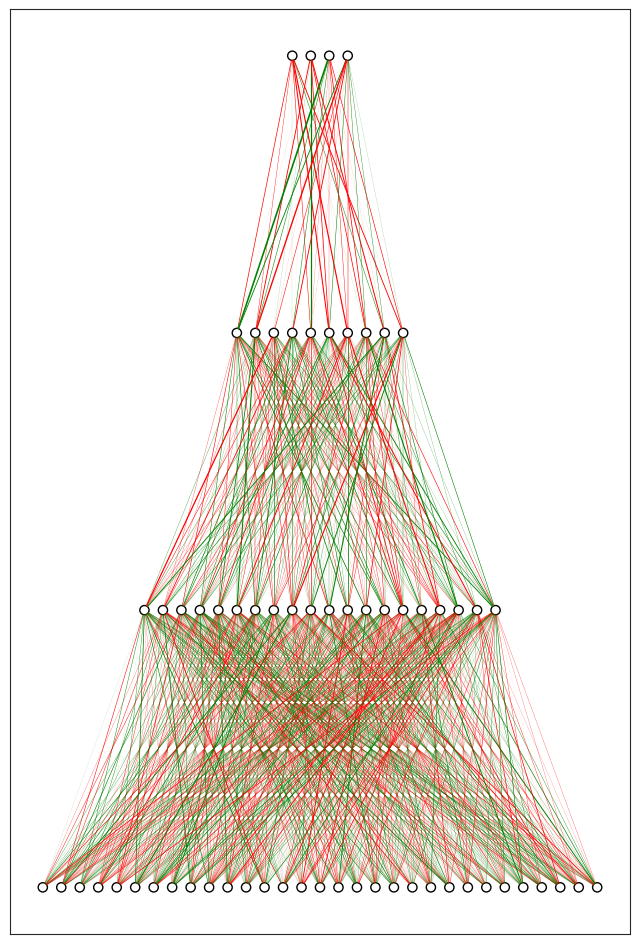
\includegraphics[width=1\textwidth]{immagini/clus_net_untrained.png}%
	}\par
	\subcaptionbox{Visualisation of the trained network topological structure with connection strengths highlighted in \textcolor{red}{red} for negative valued weights and \textcolor{green}{green} for positive values ones.\label{fig:clus_net_trained}}{%
		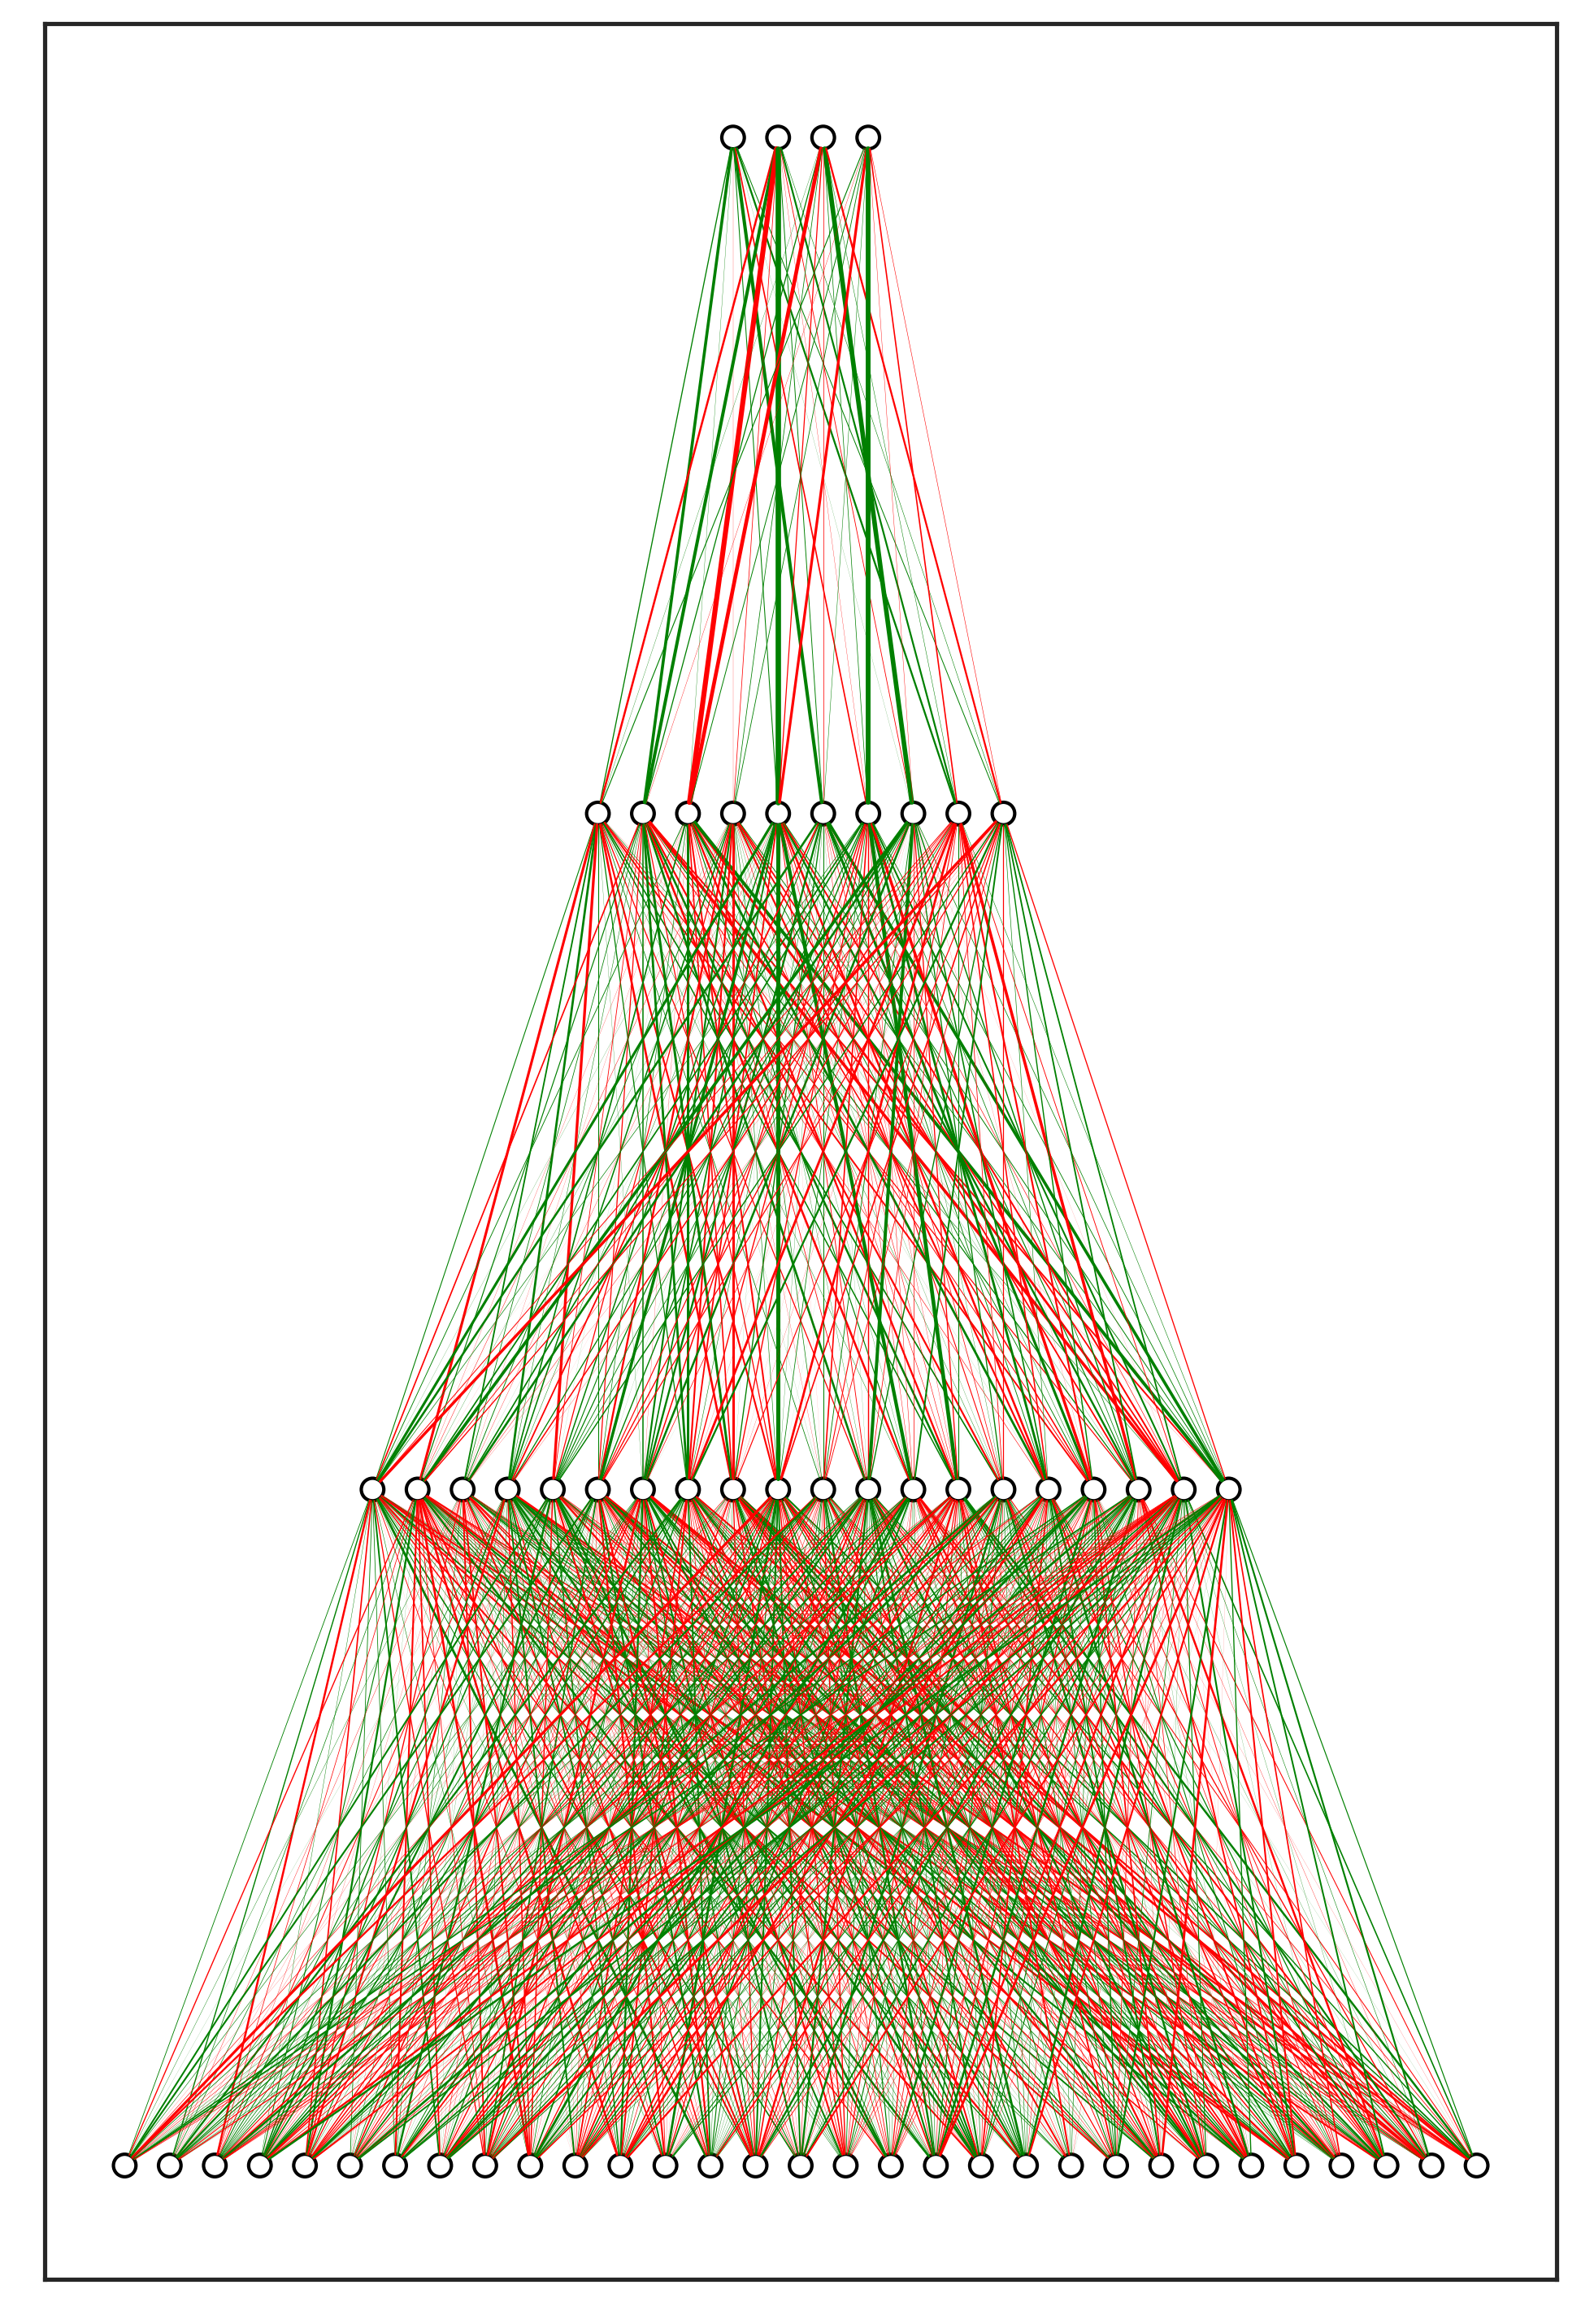
\includegraphics[width=1\textwidth]{immagini/clus_net_trained.png}%
	}
	\caption{Visualisation of the network strengths for the clusters data set.}
	\label{fig:net_clus}
\end{figure}

\begin{figure}[h!]
	\centering
	\subcaptionbox{Visualisation of the untrained network topological structure with connection strengths highlighted in \textcolor{red}{red} for negative valued weights and \textcolor{green}{green} for positive values ones.\label{fig:mvg_net_untrained}}{%
		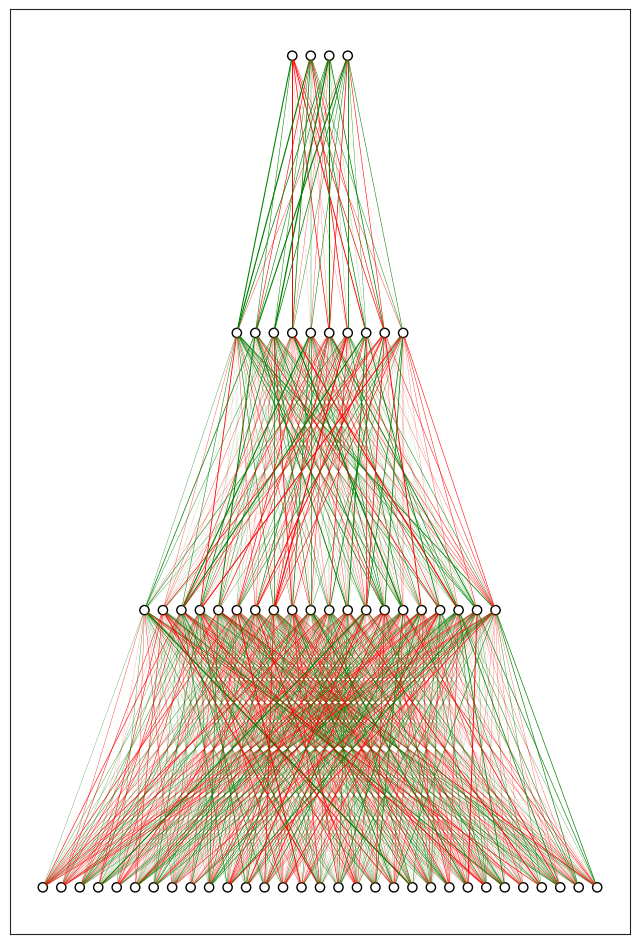
\includegraphics[width=1\textwidth]{immagini/mvg_net_untrained.png}%
	}\par
	\subcaptionbox{Visualisation of the trained network topological structure with connection strengths highlighted in \textcolor{red}{red} for negative valued weights and \textcolor{green}{green} for positive values ones.\label{fig:mvg_net_trained}}{%
		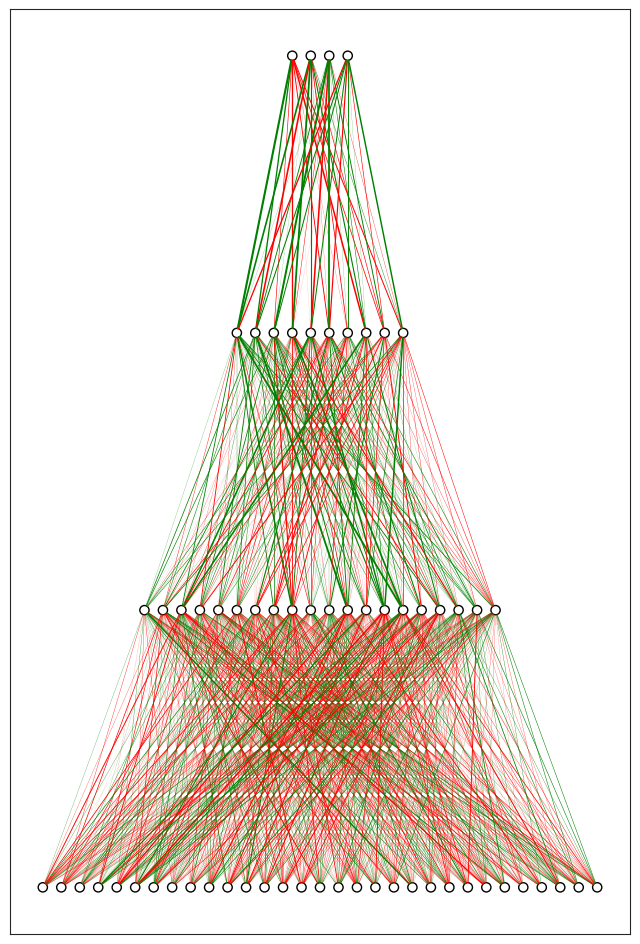
\includegraphics[width=1\textwidth]{immagini/mvg_net_trained.png}%
	}
	\caption{Visualisation of the network strengths for the MVG-training undergone system.}
	\label{fig:net_mvg}
\end{figure}

\end{document}